\documentclass[12pt]{book}


\usepackage{exercises}
\RequirePackage{lineno}
\usepackage{graphicx}
\usepackage{amsmath}
\usepackage{mathtools}
\usepackage[a4paper, total={6.3in, 8.5in}]{geometry}
\usepackage[super]{natbib}
\usepackage[autostyle]{csquotes} 

%\usepackage{siunitx}
%\usepackage[version=3]{mhchem}
%\renewcommand*{\thefootnote}{\fnsymbol{footnote}}
%\graphicspath{ {../Figures/} }
\linespread{1}

\usepackage{geometry}
 \geometry{
 a4paper,
 left=20mm,
 right=20mm,
 top=25mm,
 bottom=20mm,
 }

% Makes nice font:
\renewcommand{\familydefault}{\sfdefault}

\newcommand{\DocTitle}{Climate Dynamics Course Notes}

\usepackage{fancyhdr}
\pagestyle{fancy}
\fancyhf{}
\rhead{Mauritsen}
\chead{}
\lhead{\DocTitle}
\cfoot{}
\cfoot{}

% Remove to get numbers:
%\bibliographystyle{plainnat}
%\bibpunct{(}{)}{;}{a}{}{,}


\newcommand{\beginsupplement}{%
        \setcounter{table}{0}
        \renewcommand{\thetable}{S\arabic{table}}%
        \setcounter{figure}{0}
        \renewcommand{\thefigure}{S\arabic{figure}}%
     }

%
%\begin{document}
%
%
%\begin{center}
%\noindent
%{\LARGE 
%\DocTitle
%} \\
%\vspace{0.5 cm}
%
%\noindent
%{\bf Thorsten  Mauritsen$^{1*}$}\\
%\today \\
%\end{center}
%
%\noindent
%$^1$ Max Planck Institute for Meteorology, Hamburg, Germany \\
%%$^2$ University of Colorado, Boulder, USA \\
%%$^3$ NOAA Earth System Research Lab, Physical Sciences Division, Boulder, USA \\
%\\
%$^*$ Corresponding author: Thorsten Mauritsen, Max Planck Institute for Meteorology, Bundesstrasse 53, 20146 Hamburg, Germany, e-mail: thorsten.mauritsen@mpimet.mpg.de\\
%
%%\linenumbersK
%%\linenumbers
%%\modulolinenumbers[2]


\title{\DocTitle}
\author{Thorsten Mauritsen}
\date{\today}
 
\begin{document}
 
\maketitle
\tableofcontents



\frontmatter
\cfoot{Page \thepage}
\chapter{Preface}
Let us take a look at a planet from space -- and -- imagine we let time pass relatively quickly. From this perspective we can observe a system in approximate stationarity; something which we usually call equilibrium. This is not to be mistaken for a strict thermodynamical equilibrium, wherein, as you may have learnt in other courses, the system is characterised by a single well-defined temperature, but rather an approximate equilibrium between radiative energy received from the star around which our planet of interest is circulating (provided it does have a star), and the thermal energy that the planet is radiating to space. How does the planet come into equilibrium, and is there only one equilibrium? How does the equilibrium change if the star changes it's irradiance, or the planets orbit is altered? How does the equilibrium of the planet depend on properties of the planet? To begin to answer these questions we will have to dig into the processes that determine the energy balance, but the starting point will be our somewhat abstract perspective from space and time.

Usually we think of the climate as something that is static, we think of averages in time -- traditionally taken to be 30 years; a rather arbitrary choice as it turns out. So why discuss the dynamics of something that is static? The climate is varying on timescales as short as we choose to define them up to those of the existence of the planet. These variations were either due to external factors, such as the sun, or  the composition of the atmosphere changing due to biogeochemical processes, or internal variability. Much of this can be described by simple dynamical equations, as the dynamics of climate. A related and interesting field describes the dynamics of the atmosphere and ocean circulations, yet others their biogeochemical cycles. 

\vspace{1.0 cm}
\noindent
{\bf \LARGE Scope of the course}
\\
\\
\noindent In the Climate Dynamics course I hope to bring you close to the forefront of current knowledge in climate dynamics, and ideally to inspire you to ask interesting questions on your own. Beyond this ideal, I hope to provide you with a solid basis for appreciating the stability of Earth's climate, and how and why we think it has, and is, changing. You will learn about forcing, feedback mechanisms and climate sensitivity, about the timescales involved in the climate system, and I will have a special focus on instrumental record warming. 

The course is theoretical in the sense that we will be working with abstraction: simple models that explain some aspect of the system in a distilled way, either ignoring a number of factors or condensing them into simpler formulations. We will work both analytically and with simple computational models. 



\mainmatter
%---------------------------------------------------------------------
%---------------------------------------------------------------------
\chapter{Essentials}
\label{chapter:essentials}
Here I go over some of the basics of Earth's climatology, it's radiative properties and the energetic flows. This chapter is intended to provide a minimal background for the further studies. We will spend a bit extra time trying to understand what controls the height of the troposphere. 

\section{Temperature of the Earth and its atmosphere}
From basic thermodynamics we have learned that an isolated system has a well-defined temperature when it is in a thermodynamic equilibrium wherein there are only random brownian transfer of energy and no net fluxes exist. The Earth is very far from thermodynamic equilibrium, and instead about 173 Petawatt (PW: $10^{15}$W) are received from the sun and approximately the same amount is radiated to back to space in the form of reflected sunlight and as infrared radiation. In this case it makes sense to choose a more practical definition of Earth's temperature, for instance that temperature which is needed  needed to achieve equilibrium: the warmer it is the more infrared radiation it will radiate to space; at least in most cases. This is sometimes referred to as the Earth's radiation temperature at thermal equilibrium.

\begin{figure}
\begin{center}
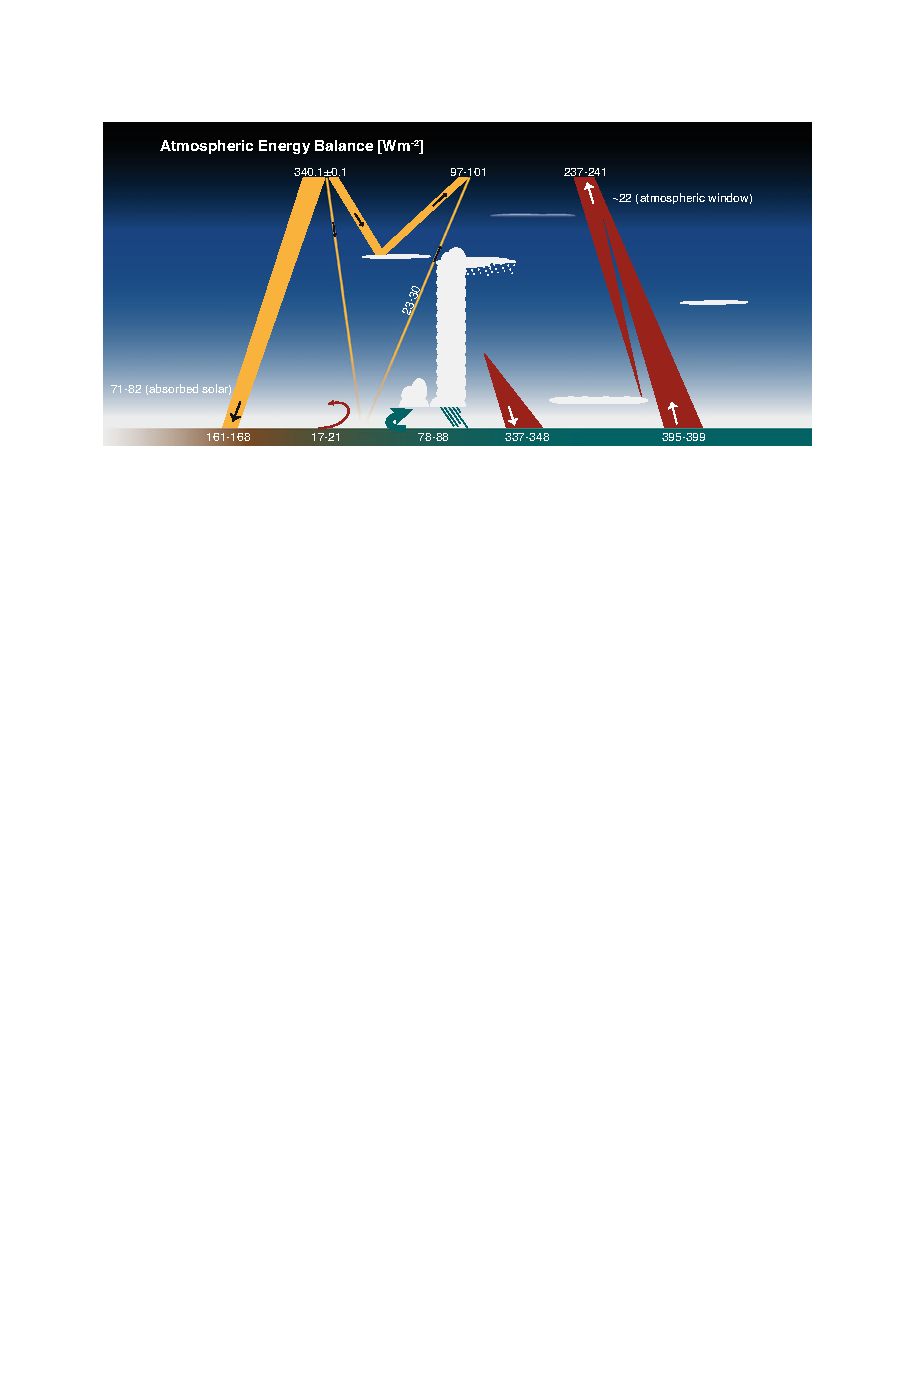
\includegraphics[width=15 cm]{../external_figures/Stevens_Schwartz_2012_energy_flows.pdf}
\end{center}
\caption{ Observational estimates of the Earth's energy balance from Stevens and Schwartz \citep{Stevens2012}. Yellow is sunlight, red is infrared radiation. The little whirl is turbulent sensible heat transfer and the green is latent heat transfer. } 
\label{fig:energy_flows}
\end{figure}

It is useful to consider the components of the global mean energy balance (Figure \ref{fig:energy_flows}). Here we consider the fluxes per meter squared surface area of the Earth (total area $510\cdot 10^{12}$ m$^2$). Energy flows in from the sun at 340 Wm$^{-2}$, about 100 of which are reflected back to space by clouds, aerosol particles or the surface. In the atmosphere some of the sunlight is absorbed, mostly by oxygen, ozone, water vapor and some by aerosol particles, and the rest reaches and heats the surface. The surface gets rid of the heat again through emitting infrared radiation, and sensible and latent heat fluxes to the atmosphere. Of the emitted nearly 400 Wm$^{-2}$ infrared radiation most is absorbed by the atmosphere.

% Danjon 1928 was first to measure Earth's reflectivity

\begin{figure}
\begin{center}
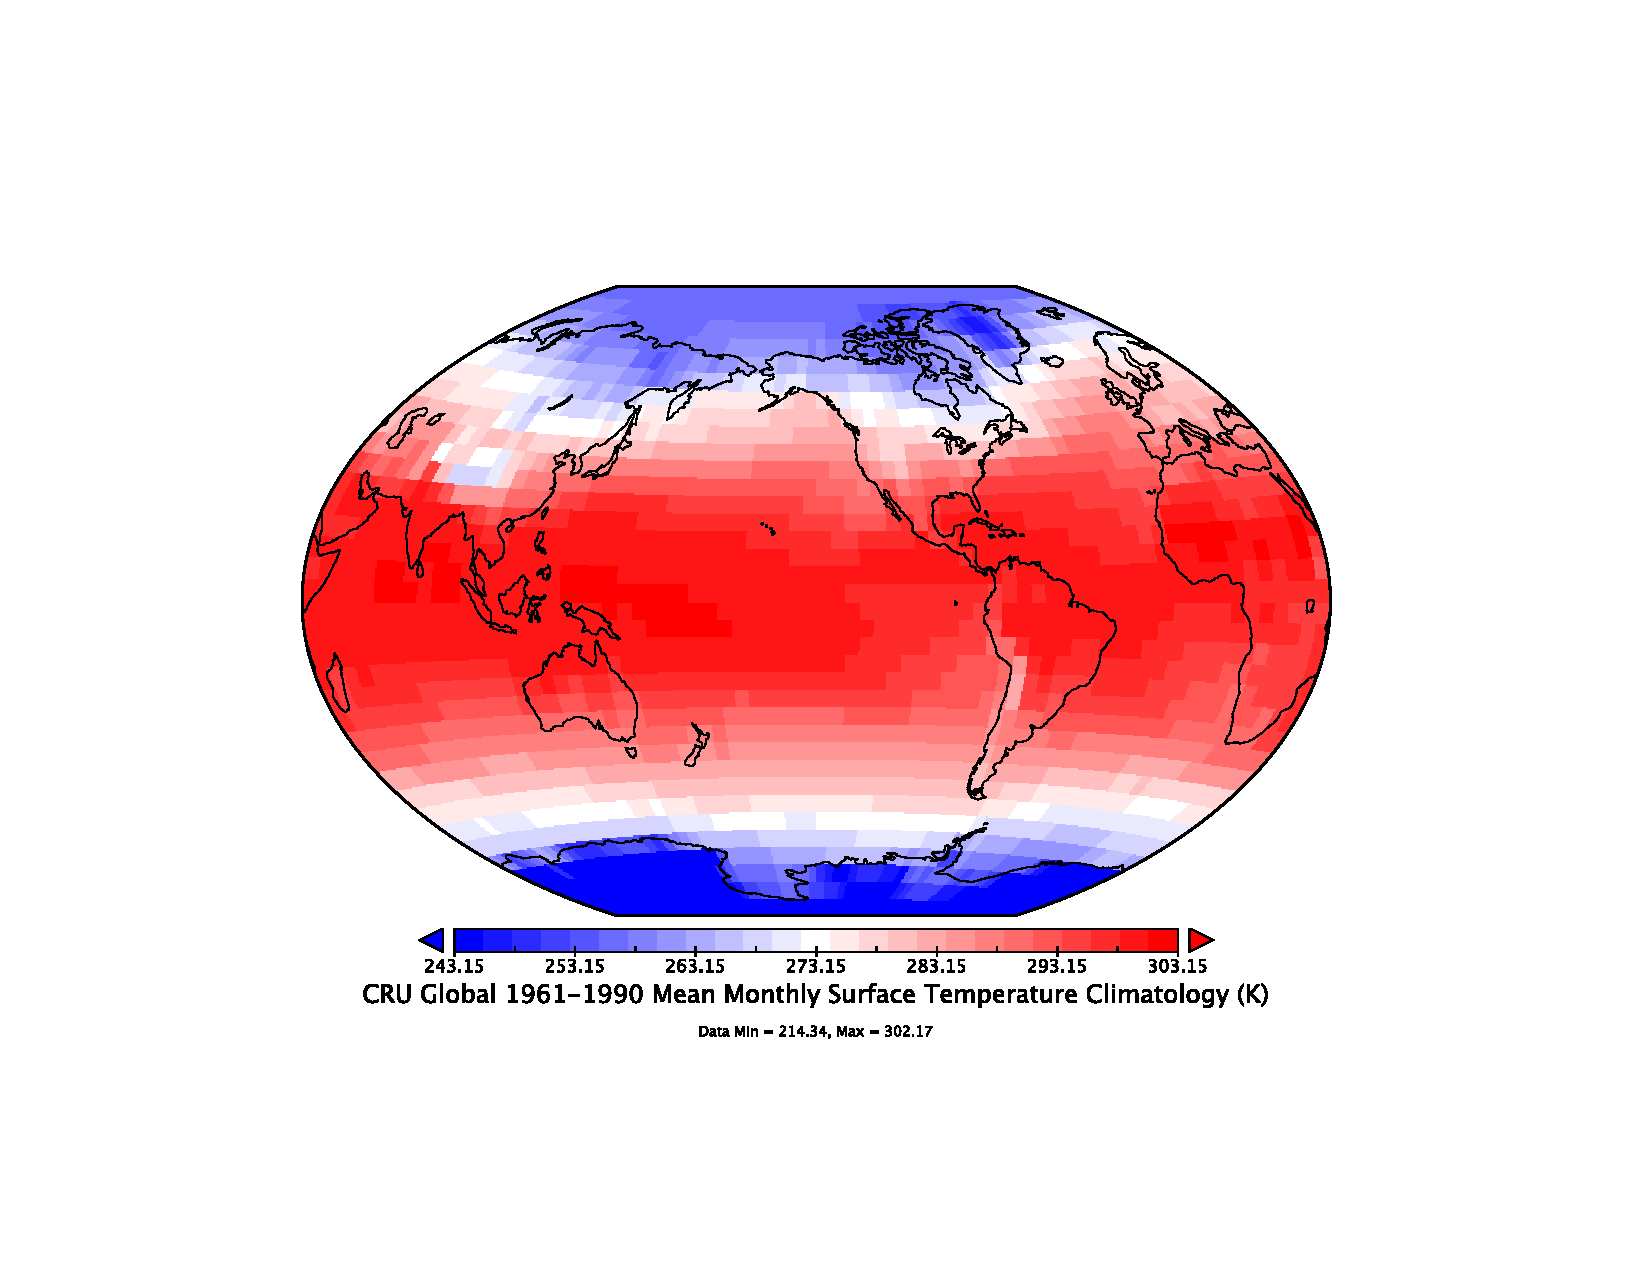
\includegraphics[width=12 cm]{../external_figures/HadCRUT_absolute_timmean.pdf}
\end{center}
\caption{ Observed annual mean near-surface temperature from HadCRUT. } 
\label{fig:HadCRUT_temperature_map}
\end{figure}

Partly because the sunlight is not distributed evenly over the Earth's surface it exhibits wildly varying temperatures near the surface with extremes from about -90$^\circ$C to +60$^\circ$C. Even in the annual longterm mean the coldest and warmest places differ by nearly 90 K (Figure \ref{fig:HadCRUT_temperature_map}). We will, however, often use a global mean surface temperature; today this is about 15$^\circ$C, or 288 K. These temperature gradients set up large energy flows in the atmosphere and oceans from warmer to colder regions. To get an idea of the magnitude of these transports one can inspect the zonal mean top-of-atmosphere radiation balance (Figure \ref{fig:ceres_fluxes}). The regions from about 36S to 36N receives more energy than is emitted back to space, whereas the high latitudes have an energy deficit. To compensate this, there must be a meridional energy transport from low to high latitudes in the oceans and in the atmosphere (It is left as an exercise to estimate the flux of energy from low to high latitudes). As a result, the temperature gradients on Earth are, in fact, modest. For instance, the Moon has equatorial temperatures varying from about 100 to 390 K between day and night, and even colder temperatures have been measured in craters near the poles.

\begin{figure}
\begin{center}
\includegraphics[width=12 cm]{../plots/CERES_Ebaf_zonalmean.pdf}
%\includegraphics[width=8 cm]{../plots/CERES_Ebaf_albedo.pdf}
\end{center}
\caption{ Top-of-atmosphere net fluxes of shortwave and longwave radiation as measured from satellite. The red area shows regions where more energy is received than emitted, it extends approximately from 36S to 36N and has a mean of 36.5 Wm$^{-2}$. The blue areas are regions that emit more radiation to space than they receive. In the Southern Hemisphere the mean flux is -54.0 Wm$^{-2}$ and in the Northern Hemisphere the deficit is -54.7 Wm$^{-2}$. Note that the x-axis is plotted as sinus of latitude such that the area under the curves can be integrated. } 
\label{fig:ceres_fluxes}
\end{figure}

On average, the coldest point in the Earth's troposphere is the tropical tropopause region with temperatures around 200 K (Figure \ref{fig:tropical_profiles}). These low temperatures are achieved through vertical mixing in deep convective clouds wherein localized rapidly rising motion causes adiabatic cooling due to the decreasing pressure with height. If the air was dry the temperature would decrease at a rate of about -10 K km$^{-1}$, but because some latent heat is released as water vapor condenses during the ascent, the actual lapse rate is less, about -6 K km$^{-1}$, tending towards the dry adiabat in the upper troposphere (Figure \ref{fig:tropical_profiles}). This is referred to as the moist adiabat. There is quite a bit more to this, some of which is also interesting to the things we will be doing in this course, but it is beyond our scope to understanding the vertical structure of the troposphere in detail.

Unlike the horizontal temperature gradients at the Earth's surface, mostly from equator to poles, that cause energy to be transported in the oceans and the atmosphere, the vertical temperature gradient of about 100 K in the topical troposphere is not on it's own causing transports to occur. However, as we shall see in a moment radiative cooling causes an upward convective  transport of energy to balance the budget of the atmosphere.

\begin{figure}
\begin{center}
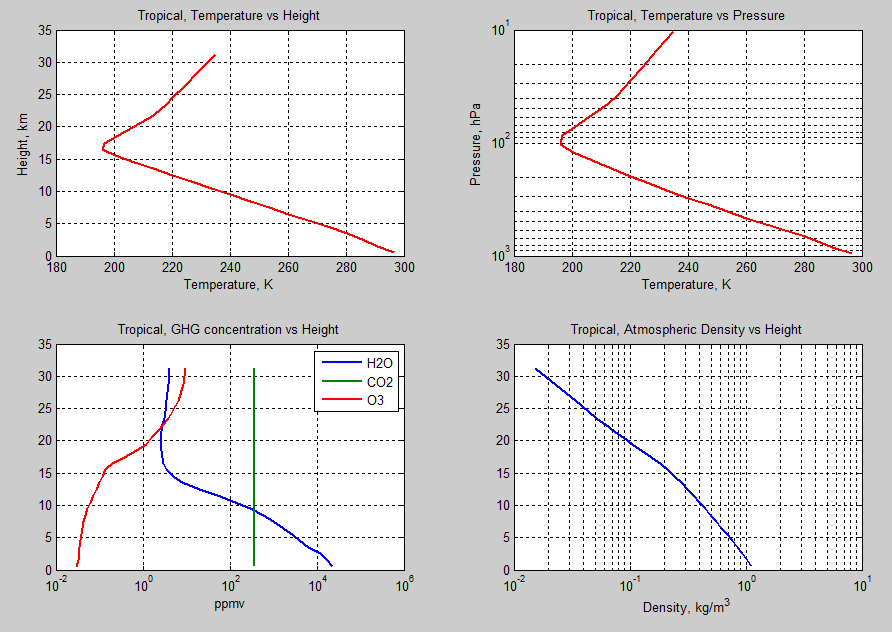
\includegraphics[width=17 cm]{../external_figures/atmospheric-radiation-13a-tropical-profile-temperature-gases-density}
\end{center}
\caption{ Typical tropical profiles of temperature as functions of height and pressure (top panels), volume mixing ratios of some greenhouse gases (lower left), and atmospheric density.  } 
\label{fig:tropical_profiles}
\end{figure}

\section{Radiative properties}
Let us next focus our attention on the infrared or longwave part of the Earth's radiation budget. A wealth of information can be obtained from studying the spectrum of radiation emitted from the Earth, stars and from other planets. This is because molecules have unique absorption properties that are determined by quantum mechanics. There are a number of ways in which atoms and molecules can absorb a photon, most of which happen at nearly discrete energies. Visible light is able to excite the electron states of atoms and highly energetic ultraviolet photons can split molecules apart. In the infrared, where photons each contain less energy, absorption happens mostly by exciting various modes of vibrations of molecules. 

Some molecules are unable to interact with infrared radiation, in fact the abundant nitrogen (N$_2$) and oxygen (O$_2$) molecules that constitute 99 percent of Earth's atmosphere are unable to absorb the low-energy infrared photons emitted by the Earth's surface. The simple configuration of these molecules with two atoms connected by electron bonds do not allow the absorption of a photon by vibration. More complex molecules with three or more atoms, such as water vapor (H$_2$O), carbon dioxide (CO$_2$), methane (CH$_4$) and ozone (O$_3$), can typically vibrate or rotate in a number of ways allowing them to absorb infrared radiation, and are therefore what we call greenhouse gases. 

A useful starting point to appreciate the information in the infrared spectrum is to consider the radiation emitted by an ideal black body which constitutes a continuous and smooth spectrum called the Planck spectrum. Ideal black bodies are not necessarily black: if warm enough they can emit visible light, instead the blackness refers to them absorbing all incoming radiation perfectly, which is necessary to obtain the ideal emission spectrum because emissivity equals absorptivity. Examples of nearly ideal black bodies are the Sun, most solids and liquids. The surface of the Earth, be it the ocean or the land, is closely approximated as a black body. A cloud is also a surprisingly good absorber: a typical low-level liquid cloud consisting of suspended tiny droplets can be a nearly ideal black body if it contains a meager 20 gm$^{-2}$ of water. Gases, on the other contrary, are usually far from ideal black bodies. 

\begin{figure}
\begin{center}
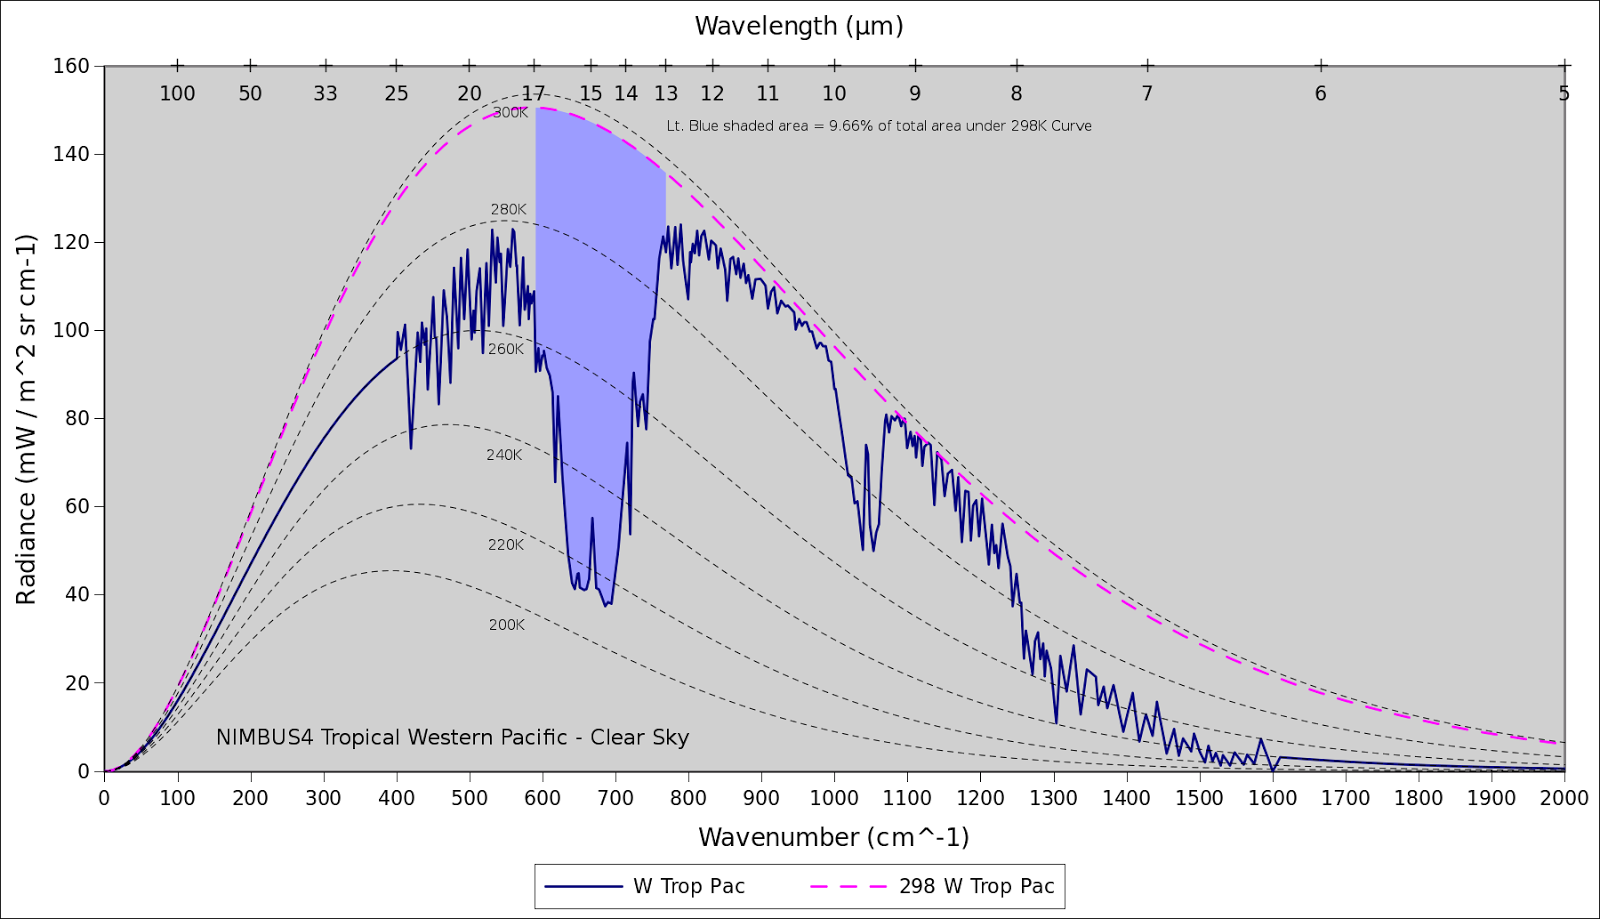
\includegraphics[width=17 cm]{../external_figures/GW_Petty_IRIS_Tropical_Western_Pacific.png}
\end{center}
\caption{ Classical irradiance spectrum measured by the infrared interferometer spectrometer (IRIS) for measuring the emission spectra of the earth/atmosphere system aboard the Nimbus-4 satellite. The instrument is limited to the range 400 to 1600 cm$^{-1}$, and outside simplistic extrapolations are made. The measurements were made in the 1970's and are restricted to clear sky scenes. Dashed lines show idealized black body spectra. Blue shading illustrates the effect of carbon dioxide (CO$_2$). The other dip at 1000-1100 cm$^{-1}$ is due to ozone (O$_3$), and the flanks (less than 600 and more than 1200 cm$^{-1}$) are dominated by vapor vapor (H$_2$O), as well as methane (CH$_4$) at around 1200-1400 cm$^{-1}$. In the atmospheric window between 10 and 13 $\mu$m there are multiple weak absorption lines from water vapor. } 
\label{fig:radiation_spectrum}
\end{figure}

Several spectra of such ideal black bodies are plotted in Figure \ref{fig:radiation_spectrum} for temperatures from 200 to 300 K as dashed lines. Also shown is the emission spectrum from a tropical cloud free scene as measured from space. The plot is linear in wavenumber such that shorter wavelength, corresponding to more energetic photons, are situated to the right. The warmer the black body the further both the peak and the tail extends to the right. For reference light that is visible to the eye is at 0.7-0.4 $\mu$m. Also the area under the spectra, which are proportional to the total irradiance from the black body which is a strong function of temperature:
\begin{equation}
R_b = -\sigma T^4,
\label{eq:blackbody}
\end{equation}
\noindent where $\sigma=5.67\cdot 10^{-8}$ Wm$^{-2}$K$^{-4}$ is the Stefan-Boltzmann constant. Most solids and liquids can be considered nearly ideal black bodies, including the Earth's surface. Also thick clouds act as if they were nearly ideal black bodies.

Now, let us compare the ideal black body spectra with the actual spectrum measured over the tropical Pacific (Figure \ref{fig:radiation_spectrum}): The observed spectrum is indeed far from ideal, which is a consequence of the atmosphere being between the satellite and the Earth's surface. Parts of the spectrum (10-13 $\mu$m), sometimes referred to as the atmospheric window, are actually quite close to the black body spectrum of the surface temperature in this tropical region (298 K), but other parts are much colder, 215 K at about 15 $\mu$m, or considerably colder with 260-270 K at both long and short wavelengths. We call these brightness temperatures as they are the equivalent irradiance of an ideal black body.
The reason that parts of the spectrum is suppressed relative to that of a black body with the surface temperature is that it is not only the surface that is emitting but also the greenhouse gases of the atmosphere absorb and emit radiation. The temperature with which they effectively emit is a result of the individual molecules absorption properties, their mixing ratio profiles, and the atmospheric density and temperature profiles (Figure \ref{fig:tropical_profiles}):
\begin{itemize}
\item
Take first carbon dioxide (CO$_2$). It has a uniform and relatively high mixing ratio and it absorbs well around 13-17 $\mu$m (Figure \ref{fig:radiation_spectrum}, blue shading). The result is that most of the emission in the band around 15 $\mu$m comes from the upper troposphere where the atmospheric density is still high enough. Above the tropopause (about 18 km) the temperature rises again, and actually some of the emission in the center of the CO$_2$ dominated band originates in the stratosphere which is somewhat warmer than the tropopause, as marked by a spike. 
\item
For the water vapor (H$_2$O) dominated flanks of the spectrum, however, the story is different. Water vapor is most abundant in the lower troposphere (Figure \ref{fig:tropical_profiles}), and most of the radiation emitted by water vapor originates from there. This results in the Earth's spectrum being closer to that of a black body with 260-270 K at the flanks consistent with temperatures at about 5-7 km in the tropics.
\item
Finally, let us consider ozone (O$_3$) which increases in mixing ratio with height and is most abundant in the stratosphere where it is produced by photodissociation of oxygen molecules by an ultraviolet photon ($\nu$): 2O$_2 +\nu$ $\rightarrow$ 2O + O$_2$ $\rightarrow$ O + O$_3$ $\rightarrow$ 2O$_2$. Most of the ozone mass is at 20-25 km altitude, whereas the volume mixing ratio peaks higher up at 30-40 km. Ozone absorbs infrared radiation at 9-10 $\mu$m wavelength where we see a brightness temperature of about 270-280 K. Most of this radiation originates from the stratosphere, which is warmer than the upper troposphere, and therefore the depression is not as deep as for the CO$_2$ case.
\end{itemize}
I hope you have now a bit of an impression of the power of the infrared spectrum. We shall return to it on later occasions. 

\section{The tropopause}
The transition zone between the troposphere and the stratosphere plays a central role in several of the themes related to the dynamics of climate. The tropopause plays a key role in determining the forcing from greenhouse gases, and it is central to understanding certain feedback mechanisms.

Perhaps a good starting point is the now iconic single-column simulations by Manabe and Strickler presented in their 1964-paper\citep{Manabe1964} (Figure \ref{fig:rce_manabe}). In their model they prescribed profiles of ozone and water vapor, and let the sun shine. A large fraction of the sunlight passes to the surface which is relatively warm. In the simplest case of a pure radiative equilibrium the surface reaches about 340 K whereas the troposphere is colder than observed. The pure radiative equilibrium is that the radiation absorbed and emitted at a given level is equal. However, in case the temperature drops this quickly with height then convective instability will occur. To parameterize this Manabe and Strickler adjusted the profile to first a dry adiabat (-10 K/km) and then to a more realistic lapse-rate close to the moist adiabat (-6.5 K/km). The result is that the troposphere is warmer and the surface is colder than at pure radiative equilibrium. Note how the stratosphere is not reacting much. Here instead the temperature rises with altitude and therefore no convective instability arises. The stratosphere also cools in the infrared, but it is being heated by absorption of sunlight mostly by the ozone layer. In summary: the convection acts to heat the troposphere in order to compensate radiative cooling -- we say it is in radiative-convective equilibrium (RCE) -- whereas the stratosphere is roughly in a radiative equilibrium. 

\begin{figure}
\begin{center}
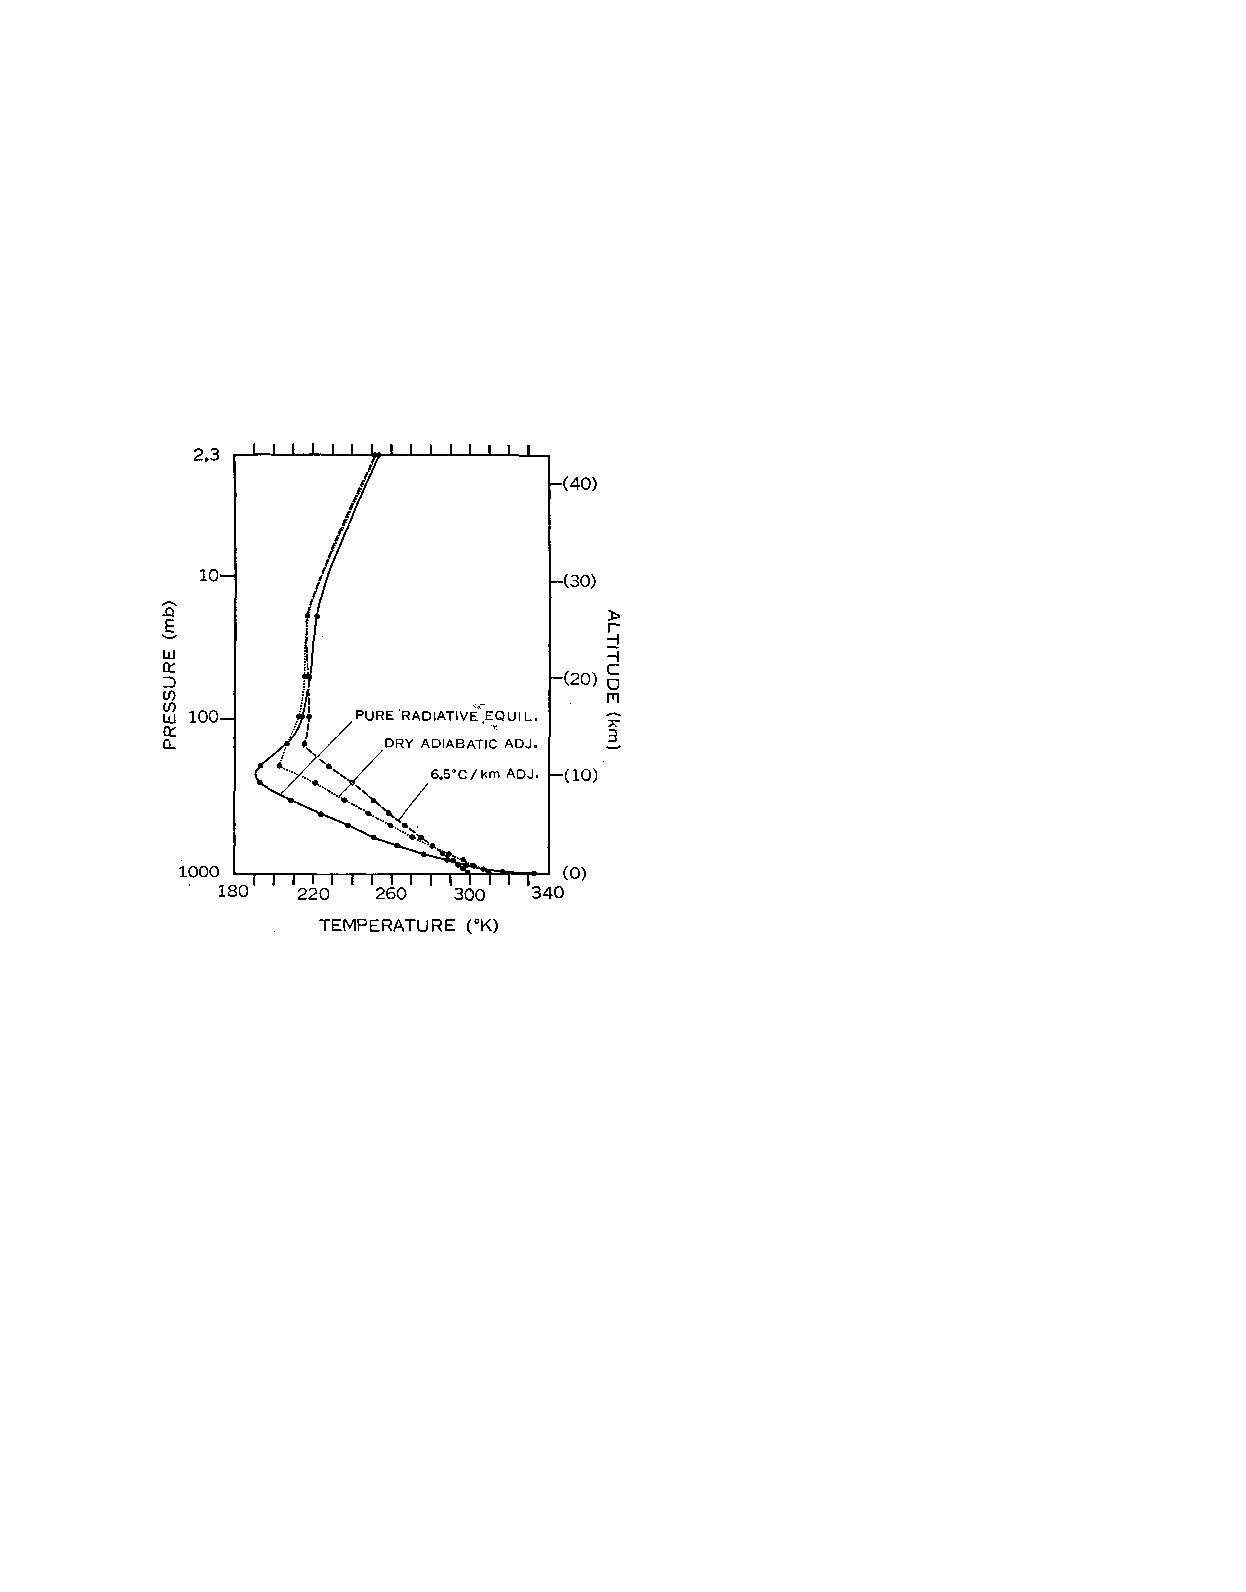
\includegraphics[width=10 cm]{../external_figures/Manabe_Strickler_1964_figure.pdf}
\end{center}
\caption{ Solutions to radiative and radiative-convective equilibrium in the single-column model by Manabe and Strickler\citep{Manabe1964}.   } 
\label{fig:rce_manabe}
\end{figure}

It is the greenhouse gases that act to cool the troposphere by emitting infrared radiation through radiative flux divergence. If we define a net flux as the difference between an upward and a downward component ($R_{net}(z) = R^\downarrow(z) - R^\uparrow(z)$, where $z$ is height), then we can calculate the heating rate as:
\begin{equation}
\frac{dT}{dt} = \frac{1}{c_p \rho}\frac{dR_{net}}{dz},
\end{equation}
where $c_p$ is the heat capacity of air and $\rho$ the density of air. Figure \ref{fig:radiative_cooling} shows infrared heating rates that are due to individual greenhouse gases in the tropical cloud-free profile displayed in Figure \ref{fig:tropical_profiles}. The heating rates are mostly negative and on the order of degrees per day, that is, if no other process would be acting to keep the temperature in place it would change at this rate. Ozone is the exception which heats the atmosphere in the lower stratosphere. But above 30 km ozone is also cooling the atmosphere, and it does so by radiating both upwards and downwards. It is partly this downwards flux from the warm upper stratosphere aloft that is being absorbed in the colder lower stratosphere. There are at least three controls that conspire to have the troposphere where it is:
\begin{itemize}
\item
Water vapor dominates infrared cooling in the troposphere, and is the reason that the pure radiative equilibrium case of Manabe and Strickler (Figure \ref{fig:rce_manabe}) has such a cold troposphere. However, water vapor mixing ratio decreases rapidly with height because the holding capacity decreases with temperature according to Clausius-Clapeyron. At around 15 km altitude, or more importantly around 200 K temperature, the cooling due to water vapor is nearly zero. It is thought that in a warming climate the tropical tropospheric temperature will increase to maintain roughly a moist adiabat, such that the level at which the temperature reaches 200 K moves upward, and with it the water vapor cooling and consequently the tropopause (Hartmann and Larsson\cite{Hartmann2002}). {\em Radiative cooling by water vapor comes to an end.}
\item
Another way to look at this is that the heating caused by moist convection, which is to compensate the radiative cooling, can only function as long as the moist and dry adiabats are different. The ascending air inside deep convective clouds follow approximately the moist adiabat which generally has a lower lapse-rate of temperature with height than the dry adiabat. The heating due to convection occurs as the surrounding air subsides instead along a dry adiabat. However, at very cold temperatures, around 200 K, the moist and dry adiabats are practically the same as there is very little water vapor left to condense, and it follows that the convection can no longer heat the troposphere. This sets another control on the tropopause height. {\em Heating by moist convection comes to an end.}
\item
Absorption of sunlight by ozone is the main source of heating in the stratosphere and results in the increasing temperature with height which hinders convection from penetrating deeper. Ozone has a relatively long lifetime in the stratosphere but if it ends up in the troposphere it is quickly destroyed. So the ozone layer has to move up to stay above a rising tropopause in a warming climate. If this leads to a thinning of the ozone layer perhaps more ultraviolet radiation can penetrate into and heat the upper troposphere, thereby increasing the temperature of the tropopause. {\em Ozone heating may bound the rise.}
\end{itemize}
Understanding the actual behavior of the tropopause is a field of active research, and the rise of the tropopause with warming plays an important role in determining climate change feedbacks. 

\begin{figure}
\begin{center}
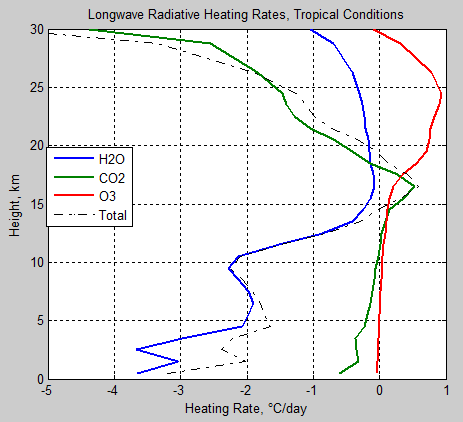
\includegraphics[width=8 cm]{../external_figures/atmospheric-radiation-13c-heating-rates-tropical-each-h2o-co2-o3.png}
\end{center}
\caption{ Longwave heating rates due to individual greenhouse gases calculated for the  clear-sky tropical atmosphere displayed in Figure \ref{fig:tropical_profiles}.  } 
\label{fig:radiative_cooling}
\end{figure}


%\section{Energy transports}
%The atmosphere and oceans transport energy

\newpage
\vspace{2 cm}
%\hrule
{\setlength{\parindent}{0cm}
\begin{exercise}
Estimate the combined poleward energy transport by the atmosphere and oceans at 36N based on Figure \ref{fig:ceres_fluxes}. Do this by estimating the area poleward of that latitude; the result should be given in PW.
\end{exercise}

\begin{exercise}
Estimate roughly from which heights in the troposphere thermal radiation to space comes from. Use Figures \ref{fig:tropical_profiles} and \ref{fig:radiation_spectrum} and divide into lower-, mid- and upper troposphere by means of its temperature. Use the fact that the area under the curve in Figure  \ref{fig:radiation_spectrum} is the total flux. %Next, compare the amount of radiation escaping to space at near-surface brightness temperature to the amount escaping through the atmospheric window in Figure \ref{fig:energy_flows}. What is the difference do you think? 
\end{exercise}

\begin{exercise}
Explain, in your own words, why the tropopause is where it is.
\end{exercise}

\begin{exercise}
Visit the MODTRAN infrared radiation model at http://climatemodels.uchicago.edu/modtran/. This is a graphical interface to a moderately resolved radiative transfer model. By default the model uses a tropical cloud-free profile with present-day greenhouse gases, and the spectrum is what one might observe looking down from 70 km altitude, i.e. at the top of the stratosphere. You can always revert to these settings by reloading the webpage. Starting from these settings, hit the {\em Save this run to background} button. The saved run will later appear as a red line. Now place yourself at the tropopause. What is the difference?
\end{exercise}
}

% TASKS:
%
% Make sure you have python access, including numpy and matplotlib (preferably Anaconda)
%
% Assume the Earth's surface is a black body and calculate it's temperature based on the emission in Figure \ref{fig:energy_flows}. Assume it is 1 K warmer, then how much more does it radiate? How much of this flux will approximately escape directly to space through the atmospheric window?
%
% Estimate from which heights in the troposphere thermal radiation to space comes from
% Estimate the fixed anvil temperature (FAT) cloud feedback by assuming a fixed areal coverage of anvils and a fixed tropospheric lapse-rate
%
% Show that the short term response to an abrupt forcing does not depend on lambda.
%
% Show that T(t) is a solution to the two-layer model to an abruptly applied forcing, draw the two components of the solution as a function of time and their sum 
% 
% Assume a polynomial behavior of lambda, estimate max and minimum ECS
% Estimate steric sea-level rise in two-layer model
% Assume X percent of the top-of-atmosphere energy imbalance goes to 
%
% Does FAT depend on the temperature of the surface?

% Imagine one alternative cause of historical warming (e.g. solar forcing, ozone depletion, geothermal heating, galactic particles). How would you go about testing this hypothesis?

%---------------------------------------------------------------------
\chapter{Energy balance}
\label{chapter:energybalance}
The flows of energy in and out of the planet is central to climate dynamics; it is actually more important to keep track of the energy balance than it is to trace surface temperature which  represents only a small part of the Earth's total heat reservoir. The temperature, however, plays a central role in determining this balance: in essence a planet receives energy at some rate and therefore warms up until it looses energy at the same rate. In fact, whereas a planet in general can receive energy in a number of ways, infrared radiation is basically the only way in which it can get rid of it again.

\section{The black body case}
Most of the Earth's energy is received from the Sun in the form of shortwave radiation, sunlight. At the Earth's distance from the Sun this corresponds to a flux of little more than 1360 Wm$^{-2}$ through a sphere centered at the Sun. This number is often referred to as the solar constant, or $S_o$, although it is not really to be considered constant. There are other small sources of energy such as geothermal heat from the interior of the Earth and heat generated by dissipation of tides, but these can be safely neglected. On other planets or moons, however, this need not be the case.

Because the distance between the Sun and the Earth is vast compared to their respective radii, we can assume that all incoming sunlight is parallel, which makes it easy to calculate the average sunlight per unit area of the Earth's surface. The radiation is intercepted by the Earth cross-section which is roughly that of a disc with the average radius of the Earth ($r$), or $\pi r^2$. But the surface area of the Earth is larger, roughly $4\pi r^2$. It follows that the intercepted sunlight must be spread over a four times larger area, giving a mean incident flux of about 340 Wm$^{-2}$. In addition, not all the incoming sunlight is absorbed, but as we saw in the previous chapter about 100 Wm$^{-2}$ is reflected back to space by clouds, aerosol particles and the surface. We say that the Earth has a planetary albedo of $\alpha \approx 100/340 \approx 0.29$. It follows that the absorbed sunlight is $R_s=(1-\alpha)S_o/4$. Finally, we shall assume that the Earth's surface has a single uniform temperature, that it radiates to space as an ideal black body following Equation \ref{eq:blackbody}, and that the atmosphere is fully transparent to infrared radiation.
Now we are in a position to form a first estimate of the energy balance ($N$) :
\begin{eqnarray}
N &=& R_s + R_b \nonumber \\ 
   &=& \frac{S_o}{4}(1-\alpha) - \sigma T_e^4,
\label{eq:black_body_energy_balance}
\end{eqnarray}
\noindent where $T_e$ is the emission temperature of the Earth that it would have had had it been an ideal black body. The balance  can be solved by setting $N=0$:
\begin{equation}
T_e = \sqrt[4]{S_o(1-\alpha)/4\sigma}. 
\end{equation}
Inserting reasonable values we obtain $T_e \approx$  255 K. This is considerably colder than the global mean surface temperature of the Earth ($T_s$) which is currently about 288 K. But remembering the observed spectrum of Earth in Figure \ref{fig:radiation_spectrum} perhaps this is not too surprising; a large part of the spectrum is at a lower brightness temperature than that of the surface. The found emission temperature is that of the ideal black body that would average the Earth's infrared radiance to space (remember the observation in Figure \ref{fig:radiation_spectrum} is a cloud-free scene from the tropics which is warmer than average).

\section{The greenhouse effect}
The reason the surface of the Earth is about 33 K warmer than the emission temperature is the so-called greenhouse effect, which was first suggested to exist by Fourier in his essay from 1827; a nice 1-page perspective on that paper is provided by Pierrehumbert \cite{Pierrehumbert2004}. Fourier formulated the question of what determines Earth's temperature and developed the idea of the planetary energy balance, which is the very foundation of climate science. 

\begin{figure}
\begin{center}
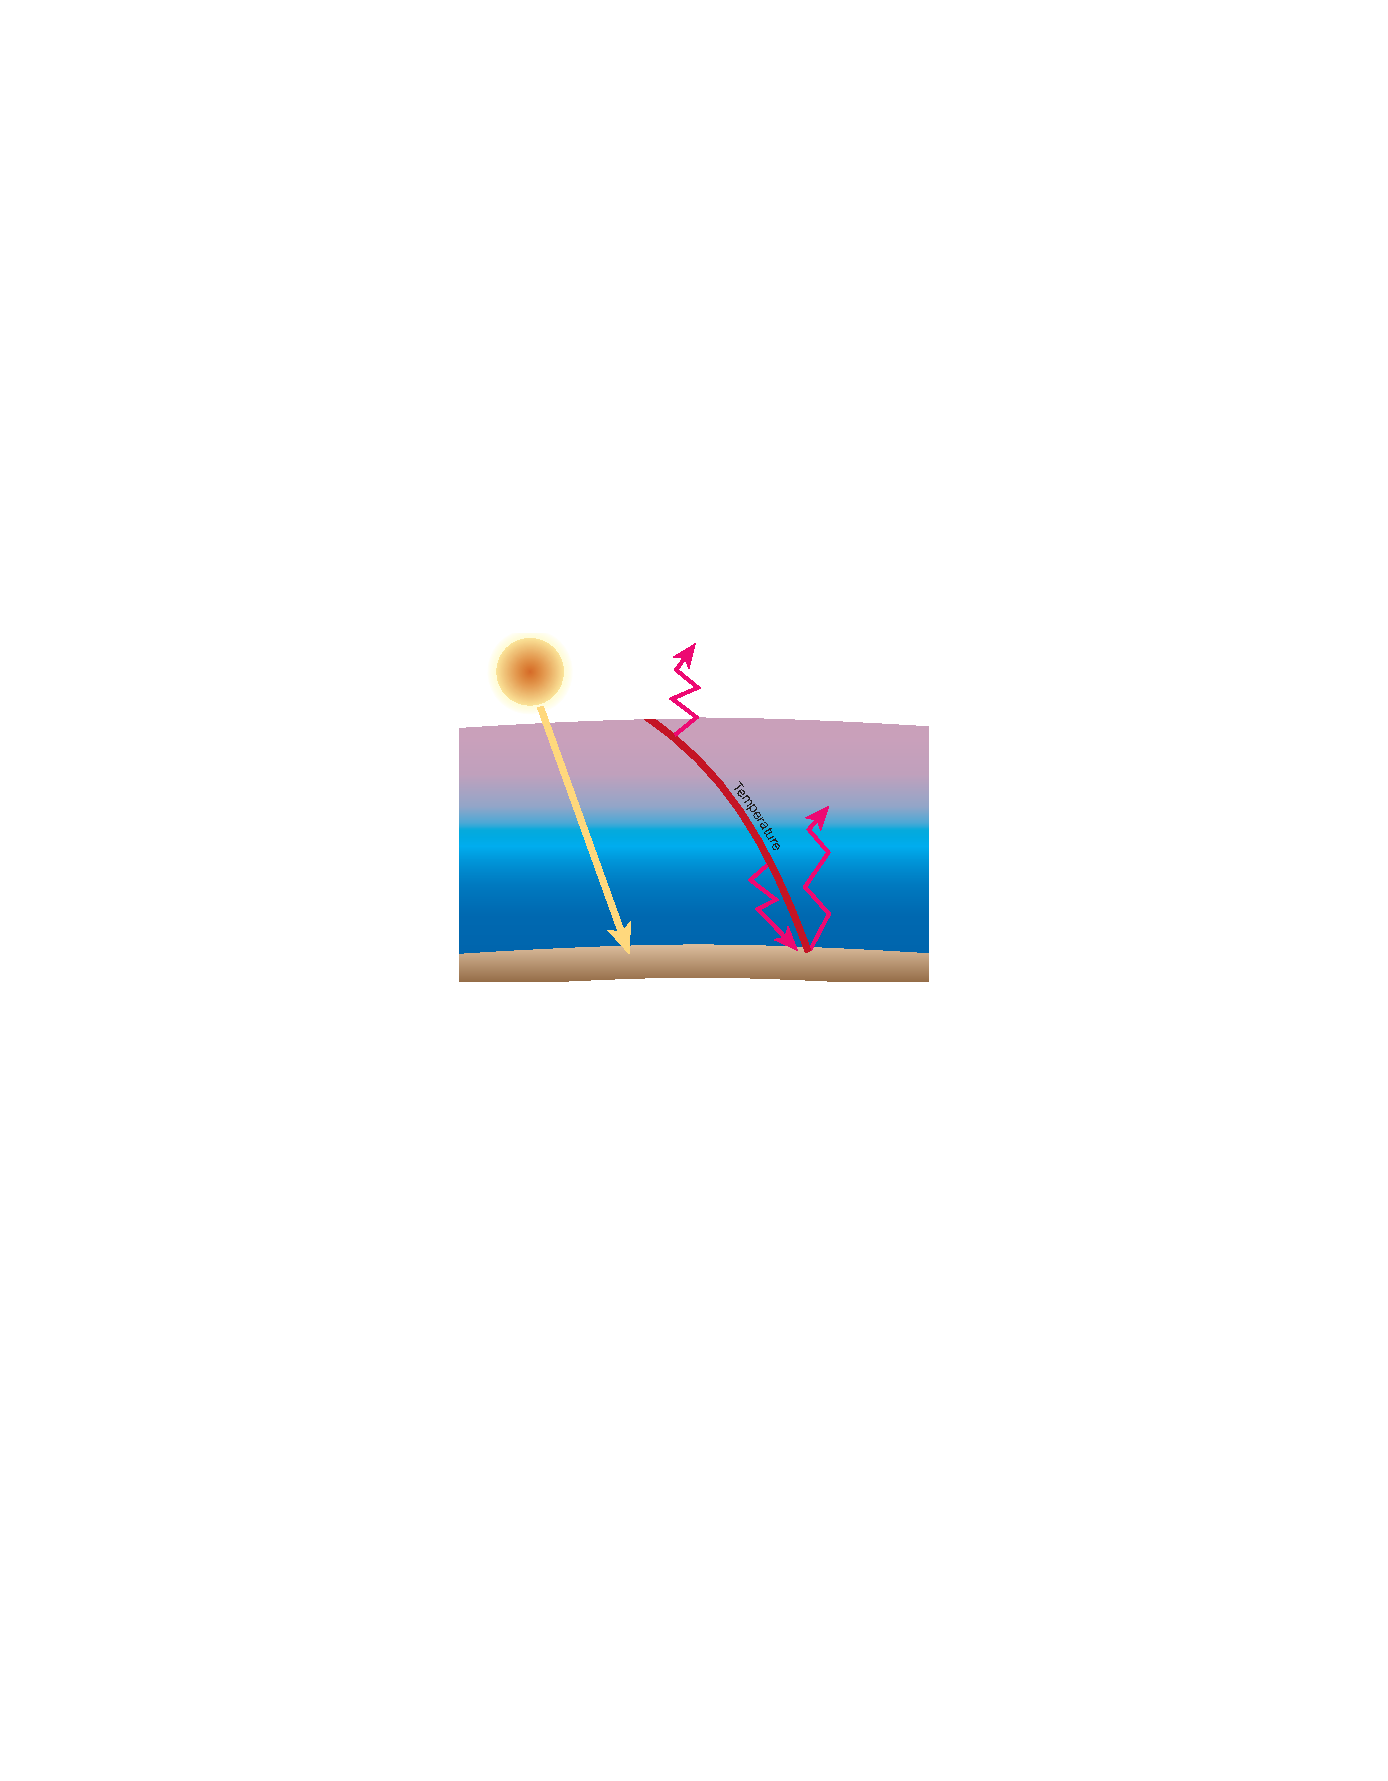
\includegraphics[width=8 cm]{../external_figures/Greenhouse_effect_illustration_Pierrehumbert_2004}
\end{center}
\caption{ Illustration of the greenhouse effect by Pierrehumbert \cite{Pierrehumbert2004}. Heat is lost by infrared radiation (pink arrows) but some of that emitted by the warm surface is absorbed and re-emitted by the cooler troposphere. The thick red line shows an idealized temperature profile. The result is that the surface has to become warmer compared to the case when there is no atmosphere in order to obtain energy balance.    } 
\label{fig:greenhouse_effect_illustration}
\end{figure}

It is often argued that the naming of the greenhouse effect is misleading. The greenhouses, which we use to grow vegetables and fruits, are indeed warmer than their surroundings because sunlight is trapped inside, but they are warmer mainly because they hinder air motion from transporting the excess heat away. This is fundamentally different from how the atmospheric greenhouse effect works which is by absorbing infrared radiation emitted by the surface and re-emitting at a lower temperature to space resulting in a warmer surface (Figure \ref{fig:greenhouse_effect_illustration}). We can define the greenhouse effect as the difference between the infrared radiation emitted by the surface ($R^\uparrow_{ir}(\textrm{sfc})$) and that which escapes to space ($R_{ir}(\textrm{toa})$), and then assume the fluxes are consistent with those of black bodies at the emission- and surface temperatures:
\begin{eqnarray}
\textrm{Greenhouse effect}&\equiv&   R_{ir}(\textrm{toa}) - R^\uparrow_{ir}(\textrm{sfc}) \nonumber \\ 
                                           &\approx&   -\sigma (T_e^4 - T_s^4) \nonumber \\
                                           &\approx& 150 \ \textrm{Wm}^{-2}, \nonumber
\end{eqnarray}
which is a bit less than the estimate by Stevens and Schwartz of 155-160 Wm$^{-2}$ (Figure \ref{fig:energy_flows}). It is easy to understand why our estimate is smaller. The black body radiation depends on the temperature to the fourth power and so if there are inhomogeneous distributed surface temperatures, such as is the case at Earth's surface ($T_s$), then the average emitted radiation is larger than that of a uniform black body with the same average temperature.

\section{The perfectly absorbing slab atmosphere}
To emulate a greenhouse effect we may consider a single-temperature, or slab, atmosphere that is perfectly transmissive to sunlight but a black body absorber in the infrared. We may think of this as a slab of perfect greenhouse gas. The atmosphere radiates up and down as an ideal black body. At the top of this atmosphere (toa) the same energy balance must hold as for the pure black body case (Eq. \ref{eq:black_body_energy_balance}). At the surface (sfc), in addition to the unhindered downwelling solar irradiance, also downwelling infrared radiation comes from the atmosphere, while the surface radiates upward: 
\begin{eqnarray}
N_\textrm{toa} &=&  \frac{S_o}{4}(1-\alpha) - \sigma T_e^4  \\ 
N_\textrm{sfc} &=&  \frac{S_o}{4}(1-\alpha) + \sigma T_e^4 - \sigma T_s^4  \nonumber
\label{eq:perfect_greenhouse}
\end{eqnarray}
and at equilibrium we have energy balances both at the top-of-atmosphere and at the surface, $N_\textrm{toa}=N_\textrm{sfc}=0$, so that we can solve for surface temperature for a single layer atmosphere:
\begin{equation}
T_s(1) = \sqrt[4]{S_o(1-\alpha)2/4\sigma}. 
\end{equation}
Putting in reasonable numbers we obtain a surface temperature of 304 K -- substantially warmer than that on Earth -- and a whopping greenhouse effect of 243 Wm$^{-2}$. Now, let us double the amount of our perfect greenhouse slab by adding another layer to obtain the solution (it is left as an exercise to show this):
\begin{equation}
T_s(2) = \sqrt[4]{S_o(1-\alpha)3/4\sigma},
\label{eq:ntwo}
\end{equation}
or in the general case with $n$ levels:
\begin{equation}
T_s(n) = \sqrt[4]{S_o(1-\alpha)(n+1)/4\sigma},
\end{equation}
such that the temperature increases monotonically with the number of perfect greenhouse slabs. Eventually, the approximations made above must break down when the surface gets so hot that it radiates visible light which can escape unhindered through this idealized atmosphere. 

Obviously, and perhaps luckily, we do not have such a perfect greenhouse slab in the Earth's atmosphere, rather individual gases only absorb in parts of the infrared spectrum. In the bands around 15 $\mu$m where CO$_2$ absorbs the atmosphere is virtually opaque to radiation, but at other wavelengths infrared radiation from the surface or lower troposphere can escape to space (Figure \ref{fig:radiation_spectrum}). It is sometimes incorrectly argued that because the atmosphere is nearly saturated in the CO$_2$ absorption bands then adding more will not act to warm the Earth's surface. However, the example above with $n$ completely opaque greenhouse gas slabs nicely illustrates the opposite: the more slabs you add, the warmer is your surface temperature.

\section{The partially absorbing slab atmosphere}
\label{sec:partially_absorbing_slab}
It is therefore useful to think of the atmosphere as partially absorbing. Commonly this is modelled using an effective emissivity that is less than unity, sometimes referred to as the gray body case, or gray radiation case. 
It is the purpose of an exercise to study this case and estimate the effective emissivity of the Earth and to show that the result is analogous to what we shall find below. 
Perhaps a physically more revealing approach is to consider an atmosphere layer analog to the perfect greenhouse case above that transmits all solar radiation but absorbs and emits in only a fraction $f$ of the infrared spectrum. The problem is illustrated in Figure \ref{fig:partially_absorbing_atmosphere}.

\begin{figure}
\begin{center}
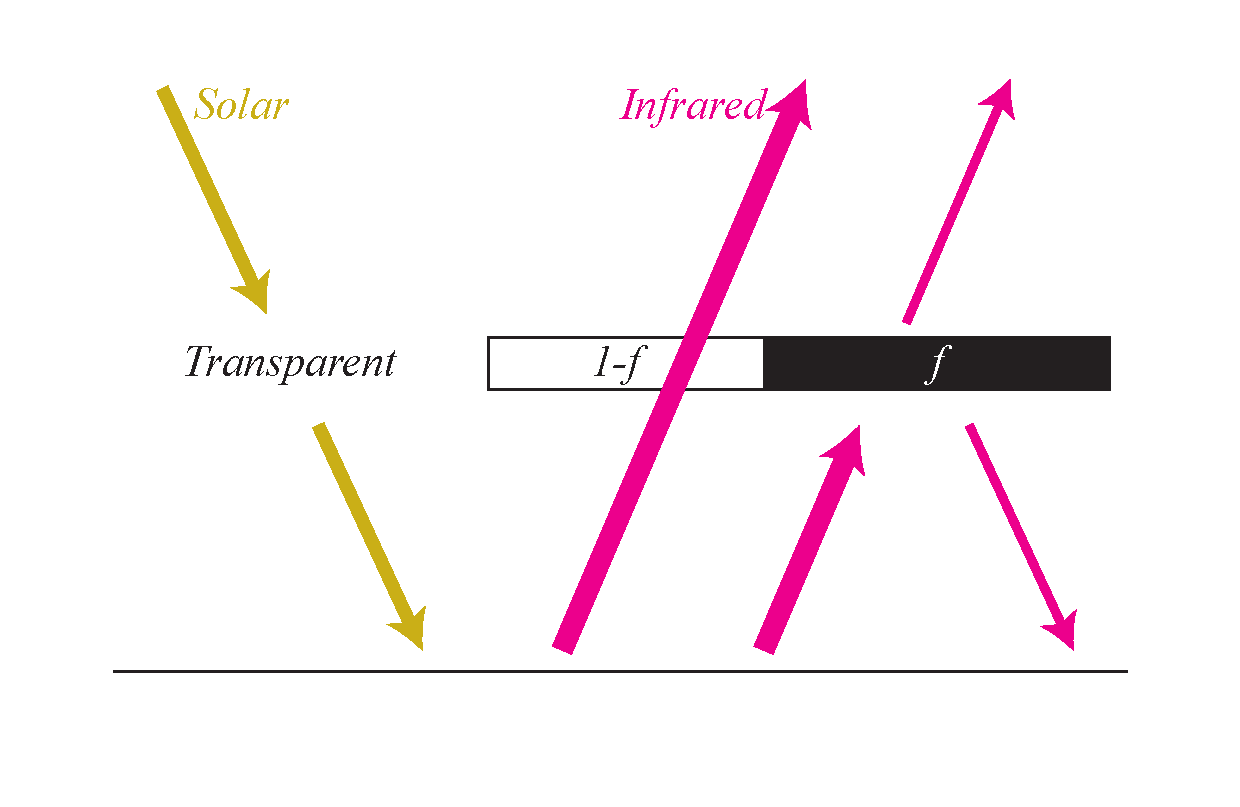
\includegraphics[width=12 cm]{../illustrations/Partially_absorbing_atmosphere}
\end{center}
\caption{ The energy balance for the partially absorbing slab atmosphere.    } 
\label{fig:partially_absorbing_atmosphere}
\end{figure}

Now, let $T_s$ be the surface temperature and $T_a$ be the atmosphere temperature. Unlike in the perfect greenhouse slab case, we cannot assume that the atmosphere temperature equals the emission temperature, $T_e$. We can then set up balances at the top of the atmosphere and at the surface:
\begin{eqnarray}
N_\textrm{toa} &=&  \frac{S_o}{4}(1-\alpha) - f \sigma T_a^4 - (1-f)\sigma T_s^4 \nonumber \\ 
N_\textrm{sfc} &=&  \frac{S_o}{4}(1-\alpha) + f \sigma T_a^4 - \sigma T_s^4 \nonumber 
\end{eqnarray}
Again, we can assume stationarity and solve for $T_s$ and $T_a$:
\begin{equation}
T_s(f) = \sqrt[4]{\frac{S_o(1-\alpha)}{2\sigma(2-f)}}, \ T_a(f) =  \sqrt[4]{\frac{S_o(1-\alpha)}{4\sigma(2-f)}},
\label{eq:partial_absorbtion_solution}
\end{equation}
such that we see that $T_s > T_a$ under all conditions and that they both increase with increasing $f$. For the limit $f \rightarrow 1$ we obtain $T_a \rightarrow T_e$ as in Equation \ref{eq:perfect_greenhouse}, and in the opposite case $f \rightarrow 0$ we obtain $T_s \rightarrow T_e$ as in the ideal black body case of Equation \ref{eq:black_body_energy_balance}. We may also solve for $f$ instead:
\begin{equation}
f = 2 - \frac{S_o(1-\alpha)}{2\sigma T_s^4},
\end{equation}
which for Earth-like conditions gives $f \approx 0.76$, that is, three quarters of the infrared radiation emitted from the surface has to be absorbed by the greenhouse slab if we are to get a surface temperature of 288 K. To obtain balance here, the atmosphere has to be colder than $T_e$, about 242 K. We can understand this as some of the radiation can escape from the surface directly space, so that to obtain energy balance with the incoming solar radiation the atmosphere has to be colder than 255 K such that the average emission temperature is $T_e$. In the limit $f \rightarrow 0$ the atmospheric temperature is about 215 K, but of course, strictly in that limit the atmospheric temperature looses meaning as no radiation is absorbed and emitted from the atmosphere anymore.


\section{Greenhouse effect of a gaseous atmosphere}
Now in practical cases the atmosphere does not consist of a single, or multiple slabs in radiative equilibrium with the incoming solar radiation and the outgoing infrared radiation, rather it consists of gases, clouds and perhaps some particulate matter. An important property of a gaseous atmosphere is that it is relatively mobile, so that it can overturn and react on timescales comparable to those of radiative heating and cooling. As a first approximation we can think of this by the troposphere having a reasonably fixed lapse-rate with height. For dry mixing this would be about -10 K/km, but as discussed earlier the real atmosphere cools less rapidly with height due to release of latent heat in convective clouds.

\begin{figure}
\begin{center}
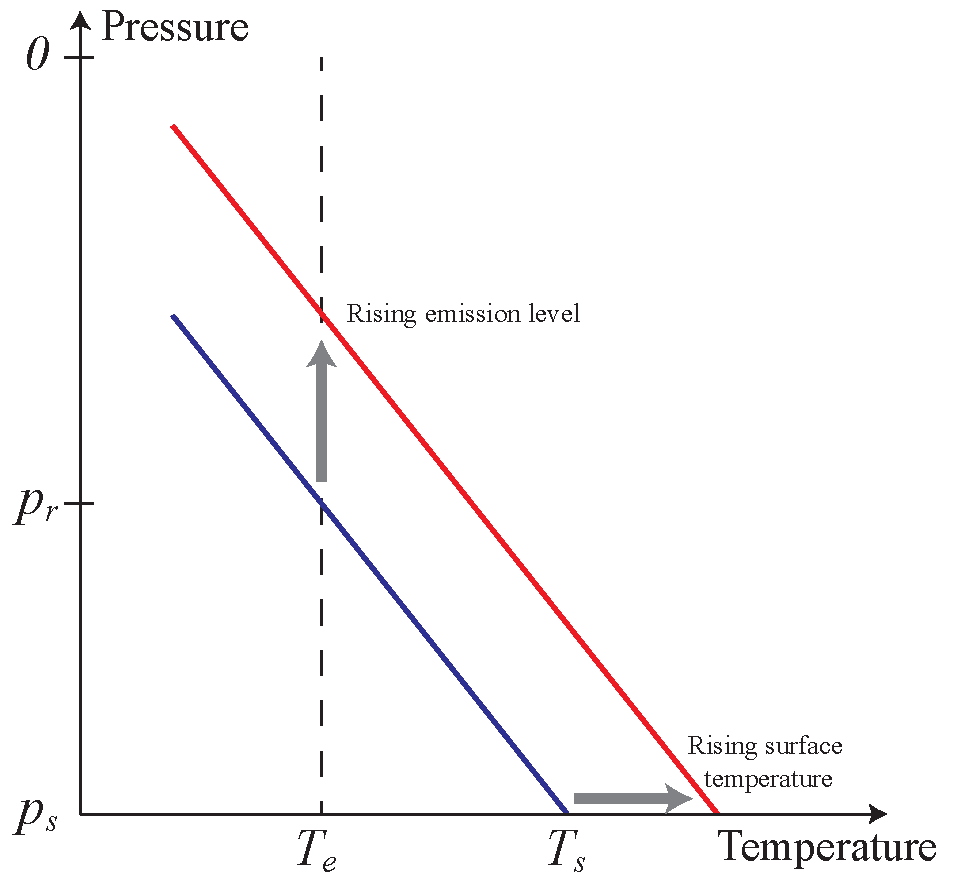
\includegraphics[width=10 cm]{../illustrations/Gaseous_atmosphere_radiation_level}
\end{center}
\caption{ Illustration of the concept of a radiation level pressure for an optically thick atmosphere. With more greenhouse gas (red) the radiation level moves upward and therefore the surface and atmosphere has to warm in order to again radiate as $-\sigma T_e$ to space.   } 
\label{fig:radiation_level}
\end{figure}

Let us start with an atmosphere that is fully transparent to infrared radiation. Here we may think of the Earth's dry atmosphere absent of carbon dioxide, ozone, methane etc. That is, it could for instance consist of nitrogen or oxygen. Then we are effectively having the black body case (Eq. \ref{eq:black_body_energy_balance}) wherein $T_s = T_e$. Then let us add some small amount of a perfect greenhouse gas, one that absorbs equally well at all infrared wavelengths. We shall assume that it is equally distributed everywhere, such as is the case for carbon dioxide (Figure \ref{fig:tropical_profiles}), with a concentration $q$. Trace gas concentrations are fractions typically measured in parts per million (ppm) or parts per billion (ppb).

As we look at this atmosphere from space the radiation emitted towards us is then  a mixture of radiation from different heights. If $q$ is very small some of the radiation emitted by the surface may escape directly to space without being absorbed by the greenhouse gas molecules: some of the photons can slip through, and we call the atmosphere optically thin. In the other limit, if $q$ is large then even a small fraction of the atmospheric column can act as if it was a black body. The pressure thickness of such a layer will scale with the amount of greenhouse molecules, $q \Delta p/g$, such that the larger $q$ is, the smaller $\Delta p$ has to be. As we view our optically thick atmosphere from space we will almost exclusively see radiation coming from the uppermost part ($\Delta p$) and it will be characterized by the temperature that prevails in this layer. In this case it may be useful to think of the infrared radiation as coming from a certain radiation level, $p_r < p_s$, that is the height at which the temperature equals the emission temperature, $T_e$. The concept is illustrated in Figure \ref{fig:radiation_level}.

As we add more greenhouse gas to our atmosphere then the pressure thickness, $\Delta p$, required to act as a black body decreases, and so with it $p_r$ becomes smaller. Therefore the emission level moves upward in the atmosphere to lower pressure. But since the emission temperature, $T_e$, is constrained to be that which closes the energy budget of the planet (in the case of Earth $T_e \approx 255$ K) then the whole atmosphere as well as the surface has to warm up. This is because the surface and atmosphere are dynamically coupled by mixing processes to follow closely a certain lapse-rate.

\blockquote{In a nutshell, the reason there is a greenhouse effect is that the atmosphere absorbs some of the radiation emitted by the surface and re-emits at a lower temperature to space. To achieve this the atmosphere has to be colder than the surface; something which is ensured through the combination of radiative atmospheric cooling and convective mixing.}

% ROUND OFF with a section arguing that greenhouse gases cause greenhouse effect if the atmosphere is colder than the surface and further that greenhouse gases, by cooling the atmosphere, ensure this to happen.


\section{A note on signs}
As you may have already noticed, throughout this set of notes I will count all fluxes as positive downwards. This has the advantage that positive fluxes will act to warm- and negative fluxes cool the system. Likewise, the feedback parameter that we shall define in the next chapter is automatically negative for stable climates and positive for unstable climates. The downside is that the {\em outgoing longwave radiation} emitted by the Earth (OLR) is then a negative flux -- where possible I shall denote it {\em net longwave radiation} trying to avoid confusion. Also note that some figures that I borrow can use the definition where OLR is positive. In the literature a number of sign conventions have developed, and it is worth paying close attention when reading on.

%\newpage
\vspace{1 cm}
{\setlength{\parindent}{0cm}
\hrule
\begin{exercise}
Show that the energy balance for the gray body case leads to this expression of the equilibrium surface temperature:
\begin{equation}
T_s = \sqrt[4]{\frac{S_o(1-\alpha)}{4\epsilon\sigma}}.
\label{eq:gray_radiation}
\end{equation}
Do this by modifying Equation \ref{eq:black_body_energy_balance} replacing $\sigma T_e^4$ with $\epsilon \sigma T_s^4$, where $\epsilon$ is the emissivity. Compare the result with the partially absorbing atmosphere, Equation \ref{eq:partial_absorbtion_solution}, and find out how $\epsilon$ depends on $f$. How small can $\epsilon$ be for a single slab atmosphere? And for $n$ slabs? Estimate the Earth's effective emissivity by solving Equation \ref{eq:gray_radiation} for $\epsilon$.
\end{exercise}

\begin{exercise}
Derive Equation \ref{eq:ntwo} for a two-layer atmosphere in the same way as done for the case for the single-layer atmosphere.
\end{exercise}

%\begin{exercise}
%Make sure you have access to a computer with Python, and follow the instructions on the handed out sheet.
%\end{exercise}

}

%---------------------------------------------------------------------
\chapter{Response to small perturbations}
\label{chapter:response}
\vspace{1 cm}

Up until now we considered climates that were stationary, at balance between the absorbed solar radiation and the emitted infrared radiation. We call this a stationary state or a fix-point. But what happens if the system is starting a bit away from that stationary state? Or what happens if we take a system in a stationary state and force it in a way that causes an energy imbalance to occur? This naturally leads us to develop the concepts of radiative forcing, climate change feedbacks and a resulting equilibrium climate sensitivity.
In this chapter we shall assume the perturbations are small such that we can linearize the system.  A surprisingly large part of the discussion around climate change is actually limited to this first-order linear regime and so it makes sense to spend some time on it. In a later chapter we shall explore systems wherein linearity can no longer be assumed and the associated concepts begin to fall apart.

\begin{figure}
\begin{center}
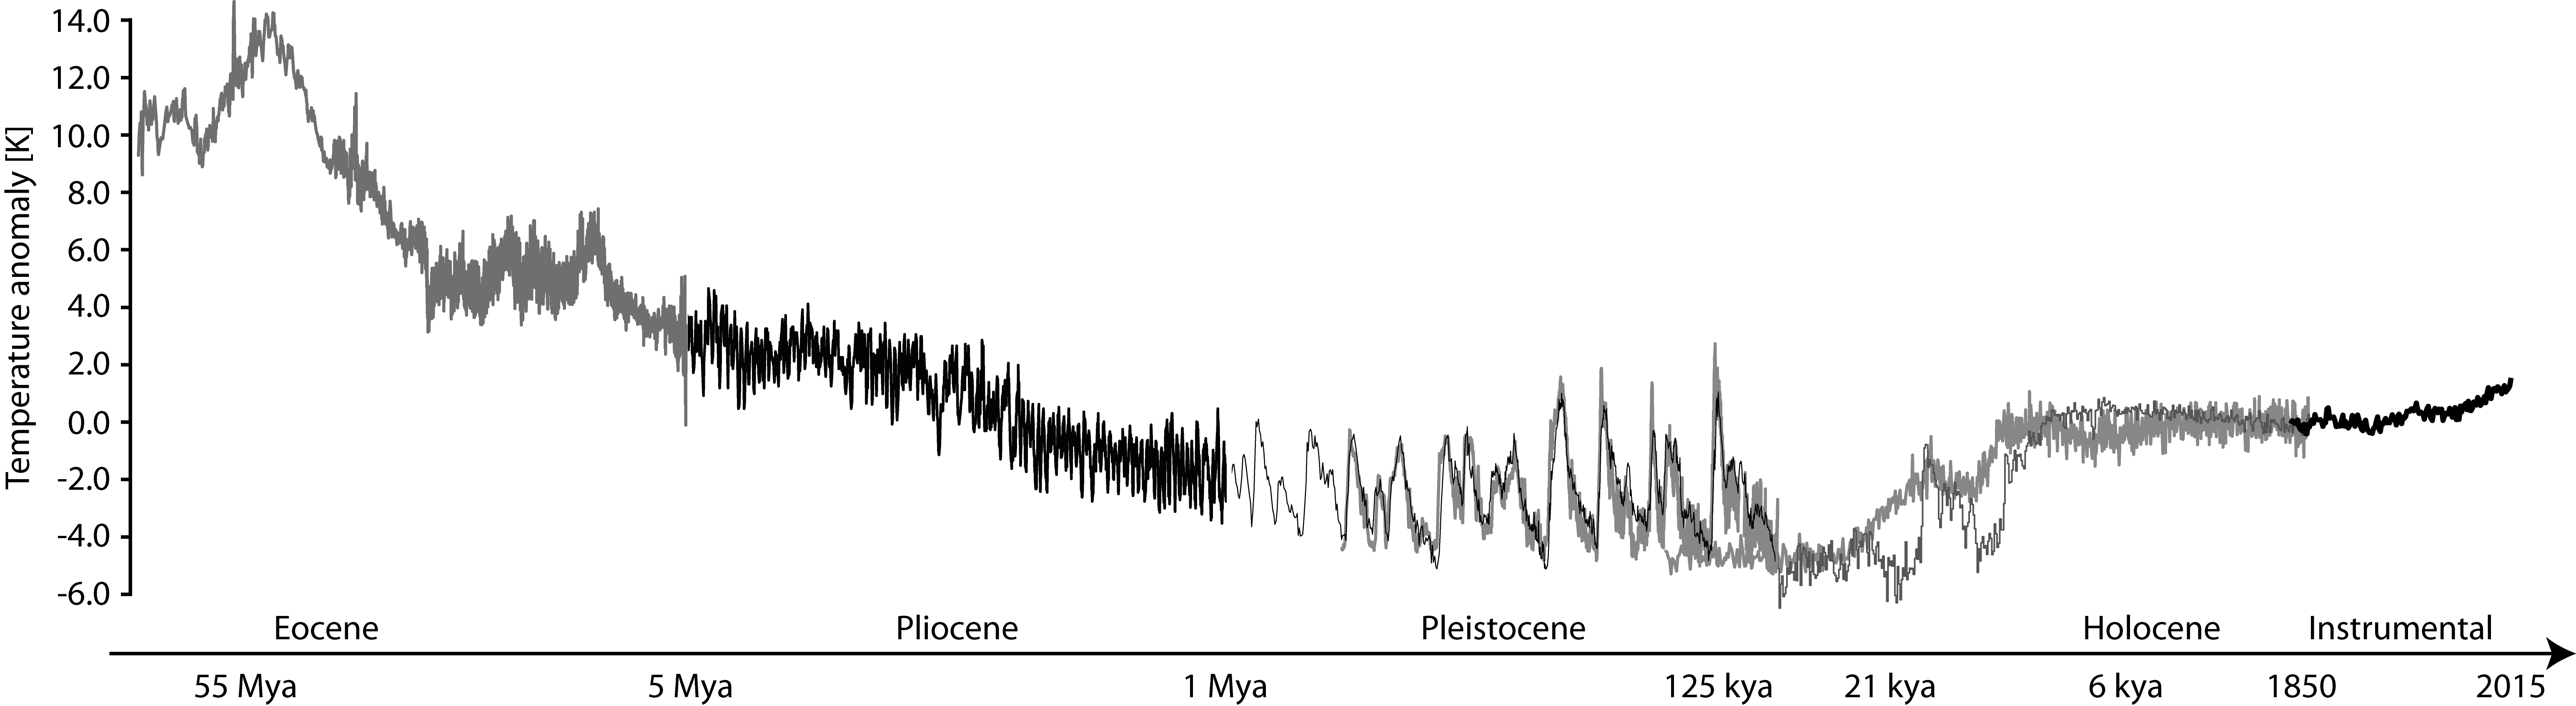
\includegraphics[width=15 cm]{../external_figures/Paleo_temperature_timeseries}
\end{center}
\caption{ Concatenation of various proxies of temperature from the past for illustration purposes. Note the logarithmic time-axis. Modified from the original by Glen Fergus. } 
\label{fig:Paleo_temperature_timeseries}
\end{figure}


\section{Climate stability}
In one perspective the Earth's climate has varied in rich ways in the past, in another perspective it has been remarkably stable (Figure \ref{fig:Paleo_temperature_timeseries}). The past 6,000 years we have had nearly steady temperatures, a period called the Holocene. These relatively mild conditions, wherein modern human civilization developed, have been rare in the past 1,000,000 years wherein the climate has cycled between longer colder glacial periods interrupted by short interglacials. Before that the Earth was warmer than it is today. For instance during Pliocene CO$_2$ concentrations were close to what they are today, about 400 ppm, and temperatures higher than during Holocene by about 2-3 K. Much earlier, during the Eocene temperatures were warmer, maybe by 10-15 K. These differences on the one hand translated into substantially different conditions for life to unfold on the planet. On the other hand, from a physical point of view the Eocene was merely 5 percent warmer than today, as measured on an absolute temperature scale. 
On this background it makes intuitive sense to think that Earth's climate is stable to small perturbations in the context of it's known history: The system did not venture to completely different states and it did spend enough time to equilibrate at almost any temperature within the range visited since dinosaurs ruled the Earth 65 million years ago (Figure \ref{fig:Paleo_temperature_timeseries}); we shall return to estimating the time-scales for equilibrating in the next chapter. It is worth pointing out though that the mere fact that temperatures did not substantially change over that period does not imply that the Earth is {\em insensitive} to perturbations, rather climate has been relatively constant due to the compensation between a longterm increase in $S_o$ and a simultaneous decrease in atmospheric CO$_2$ as carbon has been buried in fossil sediments. 

\begin{figure}
\begin{center}
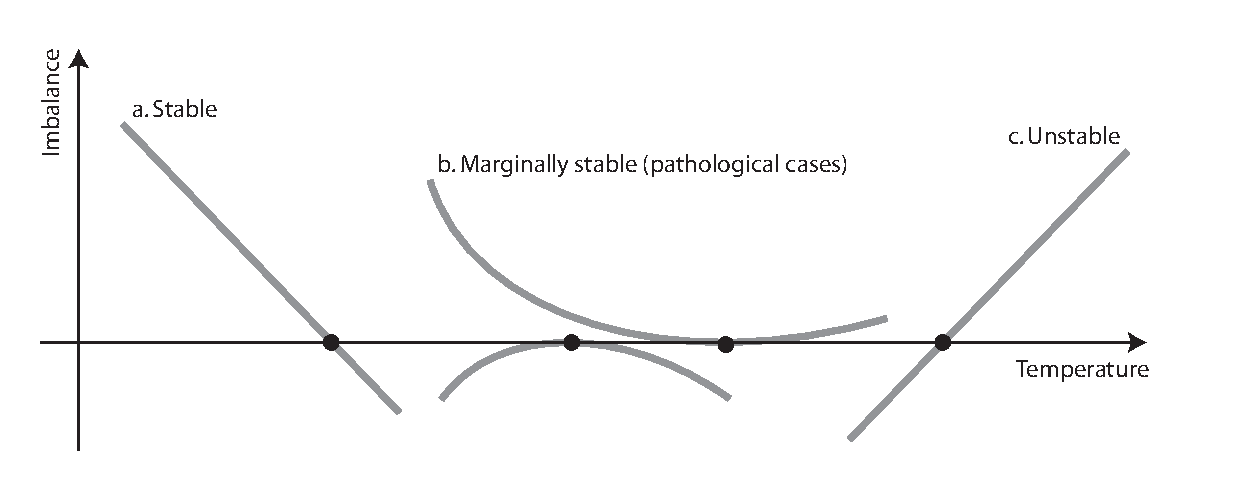
\includegraphics[width=17 cm]{../illustrations/Feedback_stability_cases.pdf}
\end{center}
\caption{ Illustration of stability cases near stationary states as marked by the black dots whereat imbalance is zero. I consider all the light gray cases where $d N/ d T = 0$ at the fix-point as limiting cases. } 
\label{fig:feedback_stability_cases}
\end{figure}

For a state to be stable it must not only have zero imbalance ($N=0$) but it must also be stable to small perturbations. The latter requires that there is some restoring force such that if the system finds itself a bit away from stationarity, then that force will act to move the system back towards the fix-point. We can think of these perturbations as arising due to internal variability, i.e weather phenomena or climate variability, or due to external forcing such as fluctuations in the solar constant or changes in atmospheric composition for reasons we consider external to the system, e.g. anthropogenic carbon dioxide emissions. For a complex system such as the Earth's climate this may be difficult to visualize as there is a practically near-infinite number of state-variables. But for many purposes we think of the climate system as having a single state-variable, the global mean surface temperature as we did it in the previous chapter, and in this case we can visualize the problem more easily (Figure \ref{fig:feedback_stability_cases}). In trying to consolidate this one-dimensional view, we may think of all the state variables as being functions of the global mean temperature. 

Now suppose $T_o$ is a fixed-point at which the imbalance is zero and that in {\em some region} above and below $T_o$ the imbalance, $N$, is a continuous and differentiable function of $T$. Then for cases wherein $dN/dT \ne 0$ the fix-points are either stable if $dN/dT < 0$, where the derivative is evaluated at $T_o$, as in some region above $T_o$ the imbalance has to be negative and the system will cool towards $T_o$, and vice-versa if the system is colder than $T_o$ it will warm up again. A similar argument can be made that the system is unstable if $dN/dT > 0$. These two possibilities are displayed as black lines in cases a and c in Figure \ref{fig:feedback_stability_cases}. We shall refer to $dN/dT$ as the feedback parameter ($\lambda$), and the above summarizes that for cases whereat $N(T_o) = 0$ the stability is determined as follows:
\begin{eqnarray}
\lambda(T_o) < 0&:& T_o \textrm{ is a stable fix-point} \nonumber \\� 
\lambda(T_o) > 0&:& T_o \textrm{ is an unstable fix-point} \nonumber
\end{eqnarray}
which is the take-home message of this section.

We talked above about stability in {\em some region} around a fix-point, but what does that mean? How large does the region have to be? It depends on how large the perturbations considered to be relevant are, if there is a faint risk of approaching another fix-point. If a stable and an unstable fix-point exists in immediate vicinity, such as shown by the dashed line in Figure \ref{fig:feedback_stability_cases}, then the stable solution is only stable to small perturbations. If it is pushed hard to temperatures above those of the unstable fix-point, then it will not return to the stable fix-point, but instead continue to warm because there $N>0$. Eventually, the system may then encounter another stable fix-point and settle at warmer temperatures. 

In the rare limiting cases wherein both $N=0$ and $dN/dT = 0$ at the fix point things get a bit more complicated. In this case it makes sense to evaluate $N$ on either side of the fix point. If $N>0$ at somewhat colder $T$ and $N<0$ at slightly warmer $T$ then the system is stable to small perturbations, as illustrated for the gray case a in Figure \ref{fig:feedback_stability_cases}. The same argument can be used for the limiting unstable case, c. In the marginally stable cases (b) wherein $N$ has the same sign on either side of the fix-point the system is stable to perturbations in one direction and unstable to perturbations in the other direction. Think of yourself as standing on a small plateau on the side of a slippery cliff. If you try to climb up the mountain you will slide back towards the plateau (stable), but if you move a bit in the other direction you fall off the cliff and never get back to your starting point (unstable). Marginally stable fix-points occur when a system undergoes so-called bifurcations, a topic we shall return to in a later chapter.

\section{The stabilizing Planck feedback}
Now let us be more concrete in applying the stability criterion we derived above. We will start with a version of the energy balance equation that you developed in an exercise of the previous chapter. In this case the greenhouse effect is represented by an effective emissivity, $\epsilon$, which is less than or equal to unity:
\begin{equation}
N = \frac{S_o}{4}(1-\alpha) - \epsilon \sigma T_s^4,
\end{equation}
from which we can estimate the feedback parameter by taking the derivative yielding:
\begin{equation}
\lambda = -\frac{S_o}{4}\frac{d\alpha}{dT_s} - \sigma T_s^4 \frac{d\epsilon}{dT_s} - 4 \epsilon \sigma T_s^3,
\label{eq:lambda_general}
\end{equation}
in the general case where $\epsilon$ and $\alpha$ are dependent on temperature. We can think of the first term as shortwave feedback which arises due to changes in planetary albedo. The origin of such feedbacks could be changes in surface albedo, e.g. through the melting of bright snow and ice, or through changes in the cloudiness and water vapor. The two other terms are infrared or longwave feedbacks. The middle term encapsulates changes in the Earth's emissivity with temperature, as we shall see e.g. due to increasing water vapor and rising upper-level clouds with warming. The last term is what is often referred to as the Planck feedback parameter.

If we consider a system with constant $\epsilon$ and $\alpha$ then the only term remaining is the Planck feedback for which we have:
\begin{equation}
\lambda_P = - 4 \epsilon \sigma T_s^3 < 0 
\label{eq:lambda_planck}
\end{equation}
for all $T_s$ implying that this system is unconditionally stable. If we insert numbers typical for the Earth we obtain $\lambda_p \approx$ -3.25 Wm$^{-2}$K$^{-1}$ which is surprisingly close to the value obtained from complex climate models, as we shall see later. The second term on the right hand side of equation \ref{eq:lambda_general}, which is broadly to be thought of as water vapor feedback (plus something called lapse-rate feedback), is found in climate models to be about +1.2 Wm$^{-2}$K$^{-1}$, and so is not sufficient to cause instability in current climates. In warmer climates the positive water vapor feedback is thought to increase faster than the negative Planck feedback and so could aid in destabilising the system. Finally, the first term on right hand side of Eq. \ref{eq:lambda_general} is the planetary albedo feedback, which is due to clouds, surface albedo as well as absorption by the atmosphere, foremost water vapor. It is left as an exercise to estimate the criterion for instability when considering planetary albedo feedback.


\section{Equilibrium climate sensitivity (ECS)}
So far we have been agnostic as to why the climate system might be out of balance. It could be due to some random fluctuation, a short volcanic eruption, a change in the solar constant, or forced by a change in the atmospheric greenhouse gas concentration. We shall return to radiative forcing in more detail later, but a standard way to define the sensitivity of the climate system is to expose it to a doubling of CO$_2$ relative to the pre-industrial level which reduces the infrared radiation to space and yields a top-of-atmosphere imbalance of:
$$F_{2x} \approx 3.7 \ \textrm{Wm}^{-2}.$$
A neat thing about CO$_2$ is that the atmosphere is optically thick in most of the spectrum that is dominated by CO$_2$ absorption. This leads to the forcing being almost logarithmic in the concentration so that each doubling (from 1 to 2xCO$_2$, from 2 to 4xCO$_2$ etc.) results in about the same amount of forcing. If we think $F_{2x}$ is a sufficiently small perturbation that the feedback parameter, $\lambda$, can be considered constant then we can write the energy balance equation as:
\begin{equation}
N = F_{2x} + \lambda \Delta T
\label{eq:linear_energy_balance}
\end{equation}
where we have linearized around a base state. Imagine that we instantaneously double the CO$_2$ concentration in the atmosphere. At this very moment we have $N=F_{2x}$ and the system will start warming. With the warming ($\Delta T > 0$) feedbacks start acting. If the system is stable ($\lambda < 0$) then the warming will lead to a reduction in the planetary imbalance ($N$). It is quite popular to think of this system as an electric feedback loop circuit (Figure \ref{fig:feedback_illustration}). 

\begin{figure}
	\begin{center}
		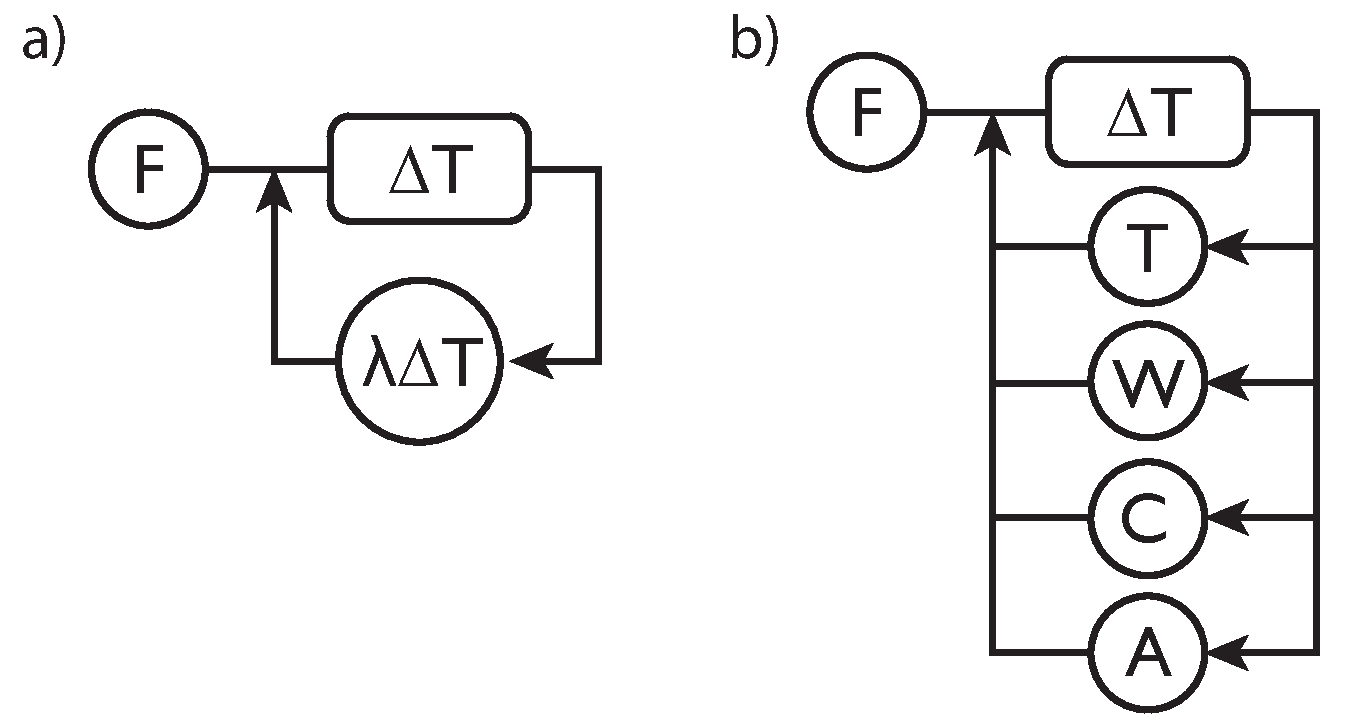
\includegraphics[width=9 cm]{../illustrations/Feedback_illustration.pdf}
	\end{center}
	\caption{ Illustration of the principle of climate change feedback to external forcing $F$. In case a) the feedback is the product of the total feedback parameter, $\lambda$, and the temperature change. In case b) I divide this into a linear sum corresponding to equation \ref{eq:lambda_linear_sum}, whereby for instance the symbol is $T=\lambda_T \Delta T$. } 
	\label{fig:feedback_illustration}
\end{figure}

Eventually, after some time, our system may reach a new equilibrium where $N=0$. Here the temperature change, which we call the equilibrium climate sensitivity (ECS) is:
\begin{equation}
\textrm{ECS} = \frac{-F_{2x}}{\lambda}.
\end{equation}
The inverse relationship between the total feedback parameter ($\lambda$) and ECS is plotted as the black curve in Figure \ref{fig:feedback_vs_ECS} along with estimates from complex climate models. %All models exhibit higher sensitivity than what would be the case if there would only be Planck feedback (dashed line). 
The scatter of models around the theoretical line can have several causes, for instance $F_{2x}$ is model-dependent and there may be non-linearities impacting the estimates. Nevertheless, most of the spread in ECS is due to spread in the total feedback parameter, and in the next section we shall further dissect this important quantity.% It is left as an exercise to explore how uncertainty in the strength of feedback mechanisms impact ECS.

\begin{figure}
	\begin{center}
		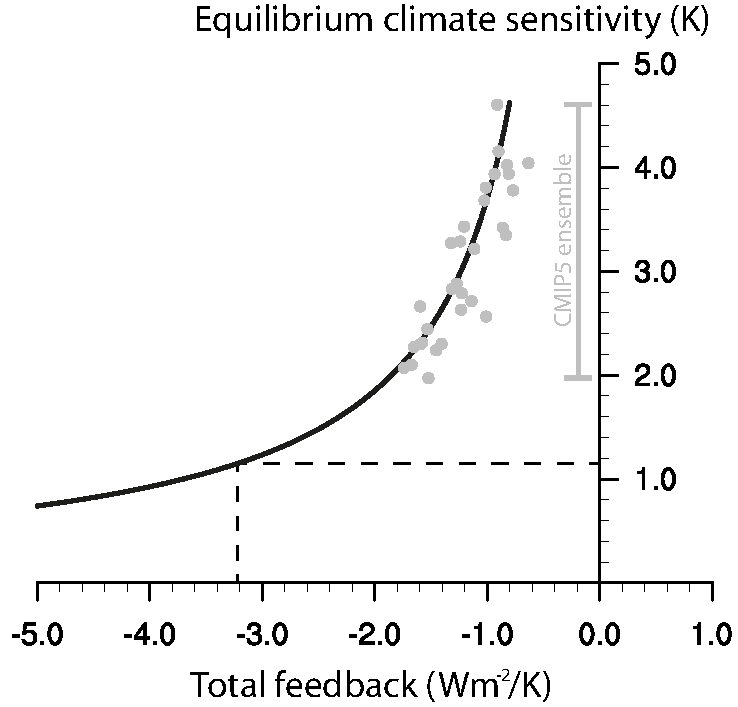
\includegraphics[width=8 cm]{../external_figures/Feedback_vs_ECS.pdf}
	\end{center}
	\caption{ Relationship between feedback and equilibrium climate sensitivity to one doubling of CO$_2$, ie. a forcing of 3.7 Wm$^{-2}$. Gray dots show individual CMIP5 climate models, and the dashed line indicates the case with only Planck feedback ($\lambda=\lambda_P$). Adapted from Mauritsen and Stevens \cite{Mauritsen2015}.} 
	\label{fig:feedback_vs_ECS}
\end{figure}






\section{Feedback mechanisms}
Above we calculated the feedback parameter for the general case (Eq. \ref{eq:lambda_general}) and identified three terms, one related to how planetary albedo changes with temperature, one related to how the effective emissivity changes and one which is directly related to the Planck feedback. Now, if we want to go about understanding and quantifying the feedback it is more convenient to make another division. For instance the planetary albedo is controlled by changes in surface albedo, cloudiness and water vapor, as well as some other factors such as aerosol particles and ozone that we shall ignore here as feedbacks. 
As a first step let us divide $\lambda$ into contributions due to changes in temperature, water vapor, clouds and surface albedo (Figure \ref{fig:feedback_illustration}b):
\begin{equation}
\lambda =  \lambda_T + \lambda_W + \lambda_C + \lambda_A + ...
\label{eq:lambda_linear_sum}
\end{equation}
where there are a number of additional terms due to interactions between e.g. clouds and water vapor changes as well as other factors that we have ignored. As long as we consider relatively small perturbations  then the interactions between feedbacks are of secondary importance. For large perturbations, however, it is easy to appreciate that this will no longer be the case. For instance at high latitudes cloudiness tends to increase in a warming climate, and so a decreasing surface albedo will have less of an impact on the energy imbalance than in a colder case. Or if the vertical temperature structure is substantially altered due to a rising tropopause, then the impacts of clouds and water vapor changes on the greenhouse effect may be different.
\begin{figure}
\begin{center}
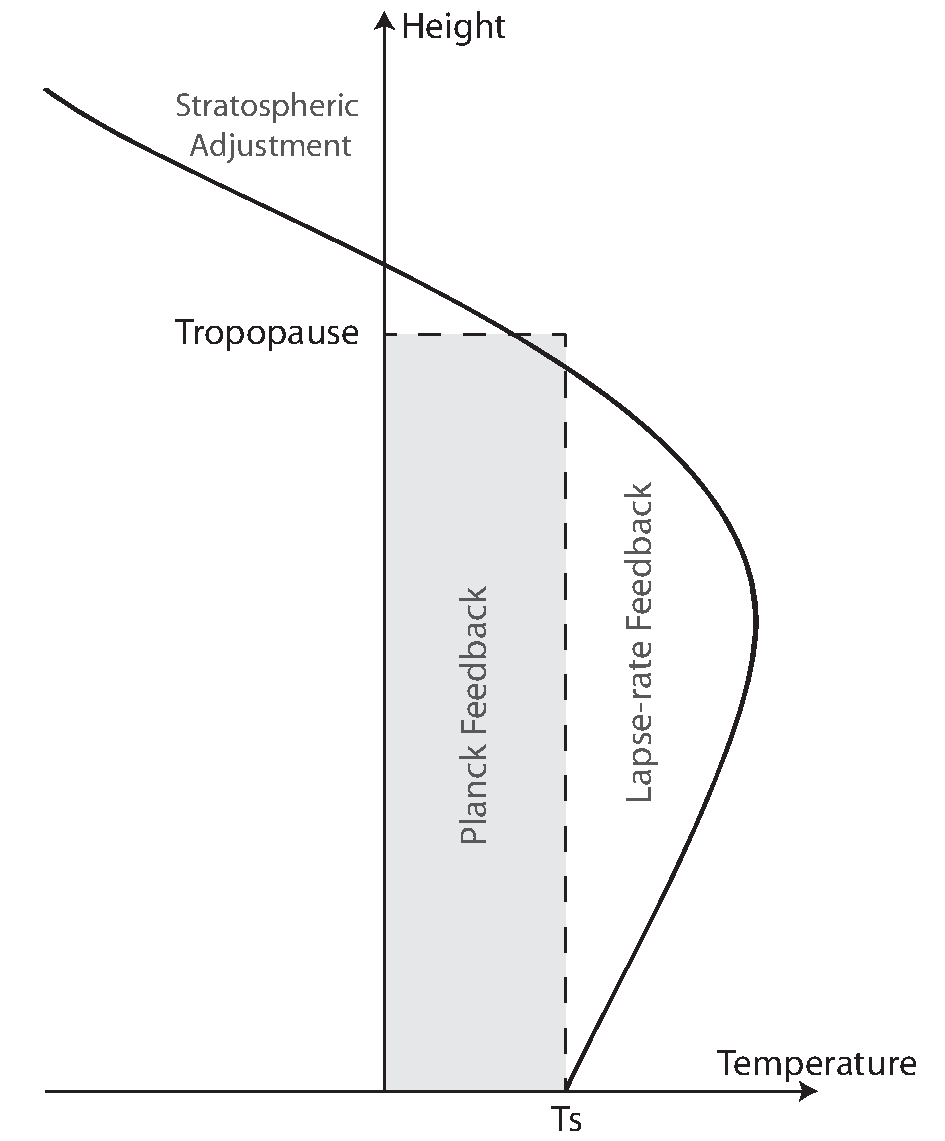
\includegraphics[width=8 cm]{../illustrations/Planck_LR_feedback.pdf}
\end{center}
\caption{ Principle of dividing temperature feedback into two contributions from Planck and Lapse-rate feedback. The shown temperature profile is typical of the tropics; at high latitudes the surface may warm faster than the troposphere. } 
\label{fig:planck_LR}
\end{figure}

It turns out to be meaningful to divide the temperature feedback parameter into two contributions (Figure \ref{fig:planck_LR}). The Planck feedback is that which would occur if the entire troposphere would warm at the rate of the surface temperature (gray shading). The lapse-rate feedback is that due to deviations from vertically uniform warming. In a later chapter we shall study stratospheric adjustment as a response to changing CO$_2$ which is not considered a feedback, and so ignoring the stratospheric temperature changes, we can write the temperature feedback as:
\begin{equation}
\lambda_T \approx \lambda_P + \lambda_{LR}.
\end{equation}
The planck feedback is therefore always negative, whereas the lapse-rate feedback could be either positive or negative: If the troposphere warms faster than the surface temperature then the system can radiate more to space relative to the case where warming was vertically uniform. This is the case in the tropics where the troposphere is vertically mixed by deep convective clouds (as in Figure \ref{fig:planck_LR}). At high latitudes, however, the surface may well warm faster than the troposphere such that the lapse-rate feedback is a positive feedback mechanism acting to amplify regional warming (Pithan and Mauritsen�\cite{Pithan2014}). However, because the tropics cover a much larger area the lapse-rate feedback is thought to be on average negative.

It is worth noting that the division of feedback parameters chosen here is only one of many possible divisions, a few of which makes sense. A powerful recent development has been to include some of the water vapor feedback into the temperature feedback, namely that which would occur if relative humidity stayed fixed (Held and Shell\cite{Held2012}). This is effective since, as we shall argue next, changes in relative humidity tend to be small in climate models. 

Complex climate models agree broadly on the importance of these feedback mechanisms, although the strengths of feedback parameters are model dependent. Table \ref{table:feedbacks} shows a dozen examples from some of the models that participated in the fifth phase of the Coupled Model Intercomparison Project (CMIP5). In particular the cloud feedback parameter varies substantially among models. An example of the spatial patterns of the feedback parameters is shown for one climate model in Figure \ref{fig:feedback_maps}. We see that the temperature feedbacks are the dominant negative feedback, whereas water vapor feedback is generally positive and strongest in the moist tropical regions. Surface albedo feedback is positive in regions were snow and sea ice melts. Finally, cloud feedbacks exhibit complex patterns which are different from model to model. Next we shall look at a some of the individual feedback mechanisms.

\begin{table}
  \caption{ Overview of feedback parameter strength (Wm$^{-2}$K$^{-1}$) in some climate models as diagnosed using the radiative kernel method. The cloud feedback parameter is split into shortwave ($\lambda_{C,SW}$) and longwave ($\lambda_{C,LW}$) contributions, and I also provide the sum of water vapor and lapse-rate feedback ($\lambda_{W+LR}$). This is a subset of the analysis from Caldwell et al.\cite{Caldwell2016}. }
  \vspace{0.5 cm}
  \centering
  \begin{tabular}{l|rrrrr|rr|r} 
Model                 & $\lambda_P$ & $\lambda_{W}$ & $\lambda_{LR}$ & $\lambda_{C}$ & $\lambda_A$ & $\lambda_{C,SW} $ & $\lambda_{C,LW}$  & $\lambda_{W+LR}$  \\
\hline
ACCESS1.3&	-3.16	&1.65&	-0.49&0.68&	0.39&	0.53&	0.15&	1.16 \\
BNU-ESM	& 	-3.08&1.46&	-0.17	&0.24&	0.56&	-0.12	&	0.36&	1.29 \\
CCSM4&	         -3.14&1.47&	-0.29	&0.27&	0.43&	0.00&	0.27&	1.18 \\
CanESM2& 	-3.22	&1.77&	-0.49	&0.54&	0.36&	-0.24	&	0.78&	1.28 \\
FGOALS-g2&	-3.15	&1.52&	-0.22	&0.39&	0.54&	0.00&	0.39&	1.30 \\
GFDL-CM3&	-3.12	&1.67&	-0.64	&0.92&	0.40&	0.64&	0.28&	1.03 \\
HadGEM2-ES&	-3.13	&1.62&	-0.41	&0.73&	0.35&	0.31&	0.42&	1.21 \\
IPSL-CM5A-LR	&-3.19&2.02&	-0.94	&1.17&	0.23&	0.63&	0.54&	1.08 \\
MIROC5& 	-3.19	&1.86&	-0.67	&0.00&	0.42&	-0.32	&	0.32&	1.19 \\
MPI-ESM-LR&	-3.10	&1.80&	-0.80	&0.46&	0.39&	-0.14	&	0.60&	1.00 \\
MRI-CGCM3&	-3.19	&1.49&	-0.34	&0.30&	0.45&	0.30&	0.00&	1.15 \\
NorESM1-M&	-3.11	&1.48&	-0.23	&0.35&	0.39&	0.07&	0.28&	1.25 \\
INM-CM4.0&	-3.11	&1.59&	-0.43	&0.23&	0.38&	0.01&	0.22&	1.16 \\
\hline								
Ensemble mean&	-3.15&	1.65&	-0.47&	0.48&	0.41&	0.13&	0.35&	1.18 \\
Standard deviation&	0.04&	0.17&	0.24&	0.32&	0.08&	0.32&	0.20&	0.10
  \end{tabular}
  \label{table:feedbacks}
\end{table}



\begin{figure}
\begin{center}
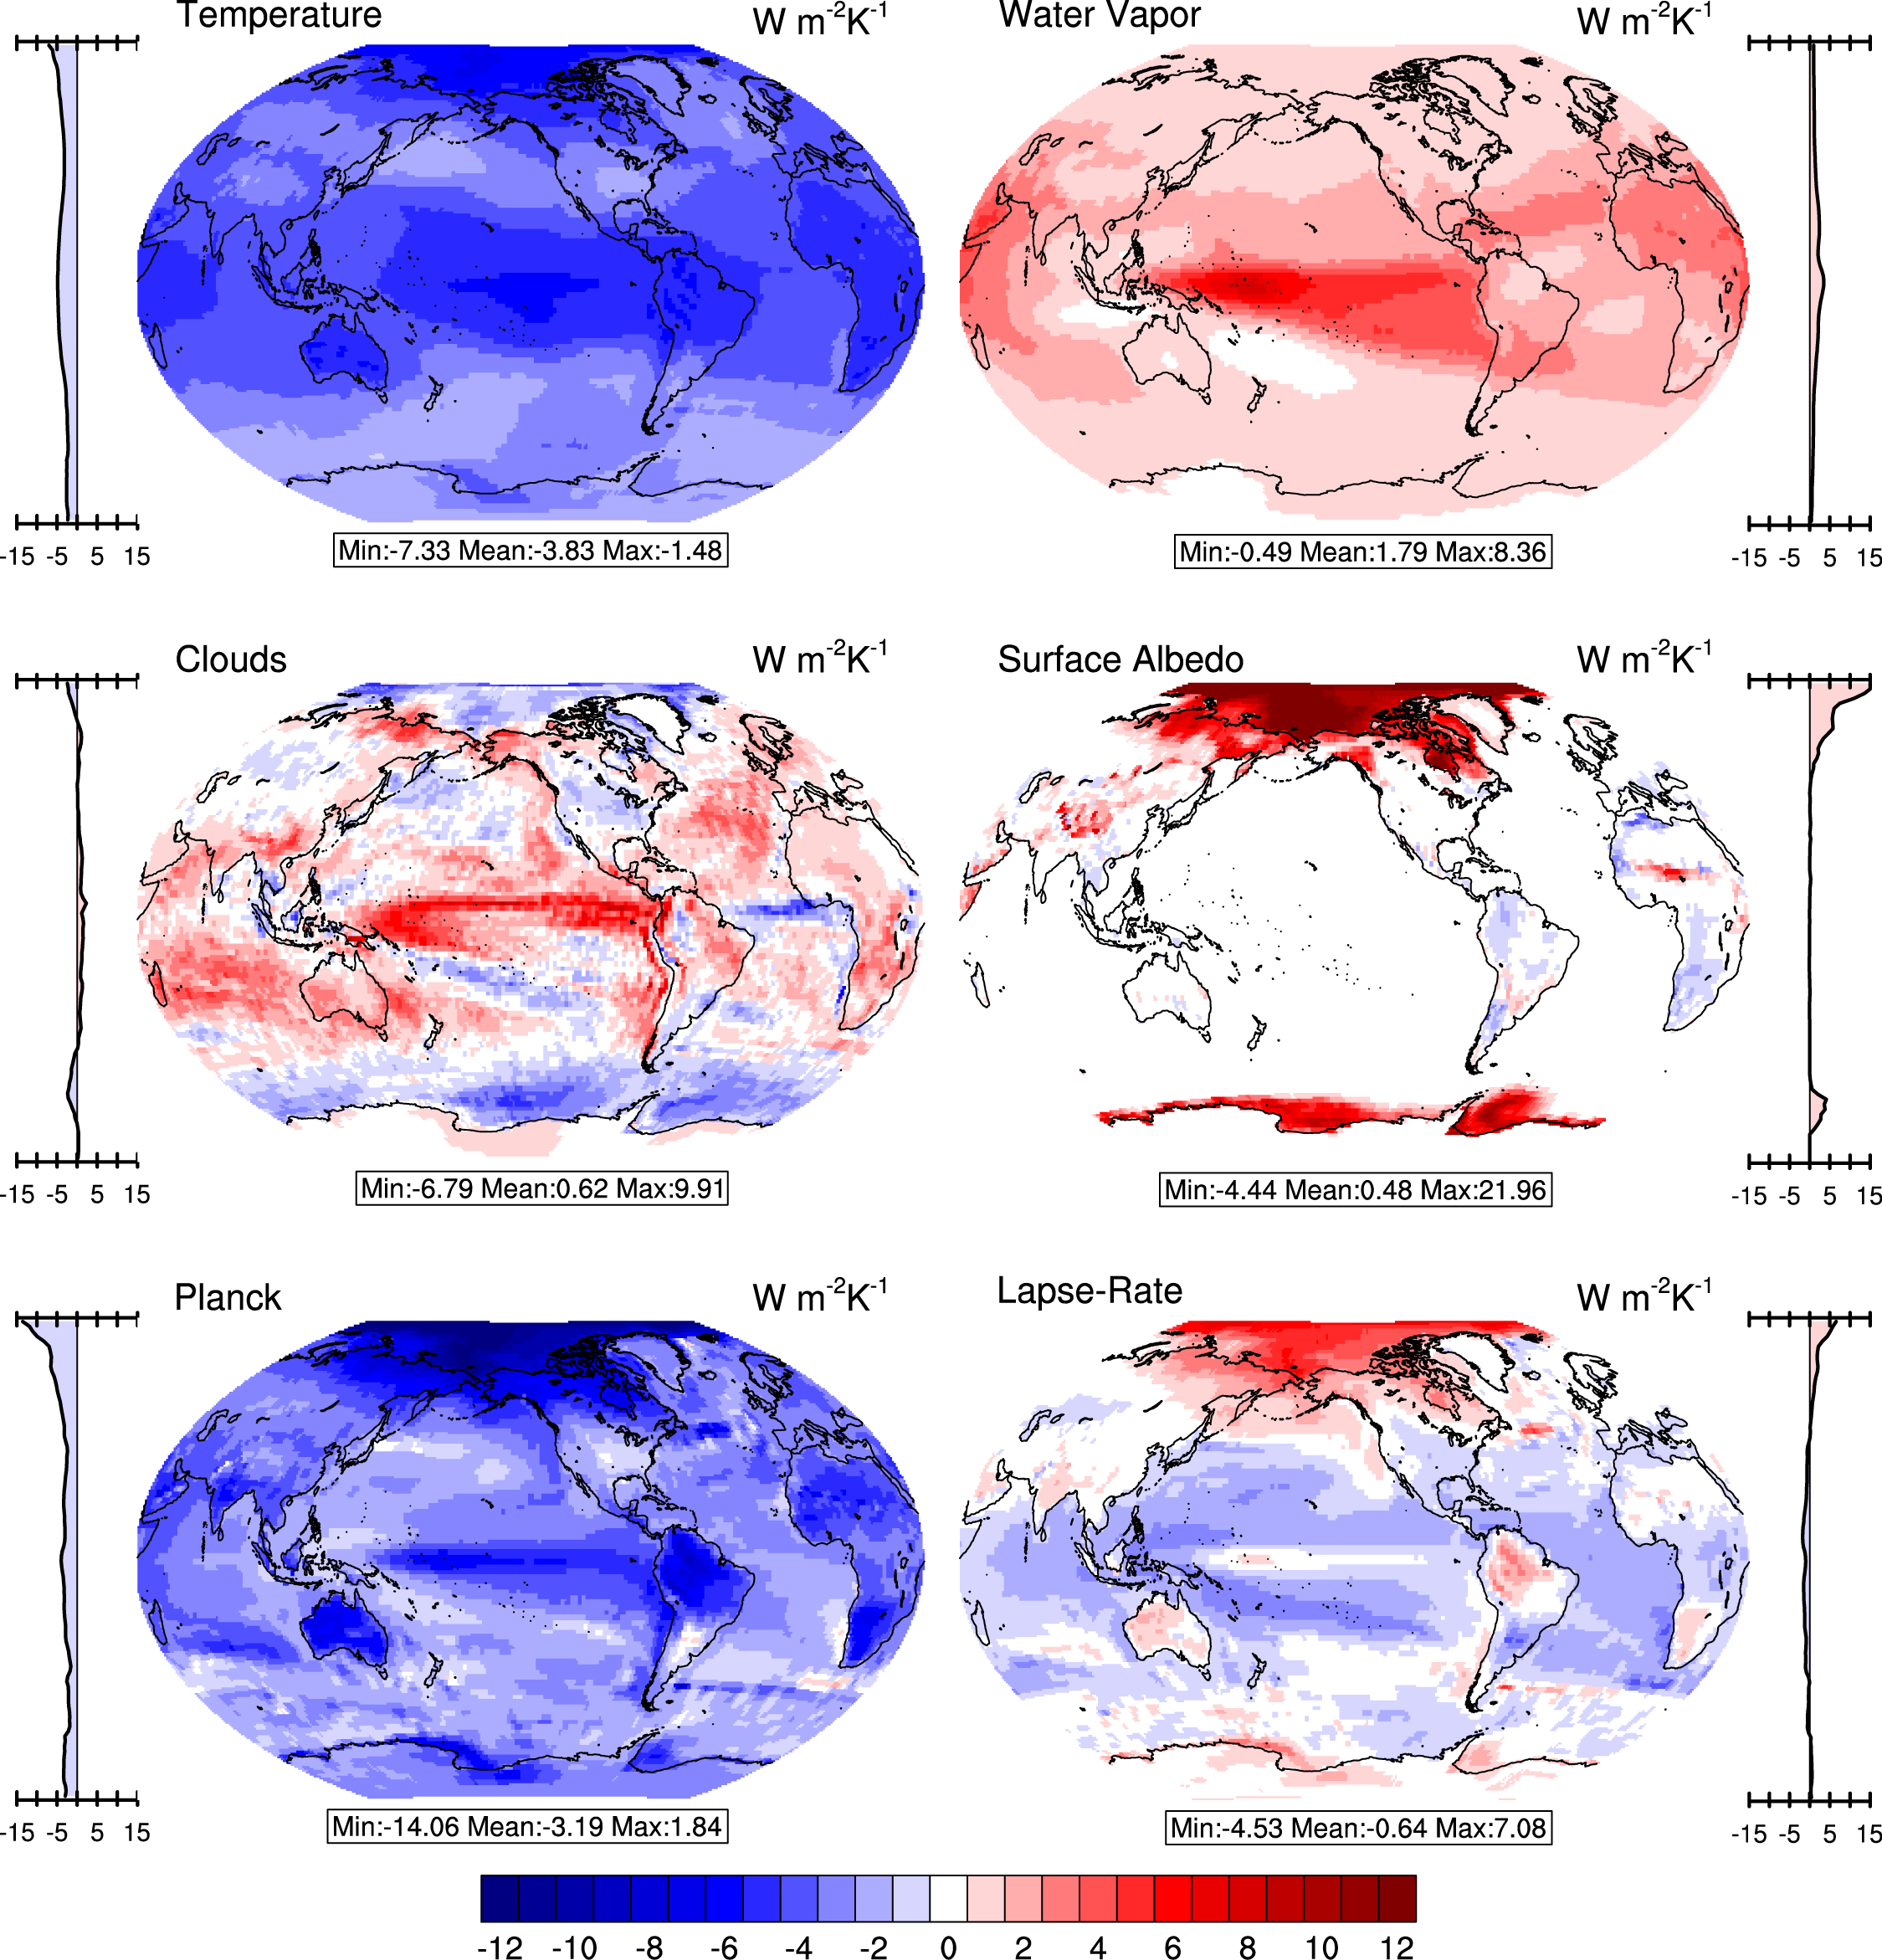
\includegraphics[width=15 cm]{../external_figures/MPI-ESM_abrupt4xCO2_allfeedbacks_contour.png}
\end{center}
\caption{ Maps of feedback from MPI-ESM-LR, from Block and Mauritsen \cite{Block2013}. } 
\label{fig:feedback_maps}
\end{figure}

\subsection{Surface albedo feedback}
Perhaps the simplest feedback to comprehend is the surface albedo feedback. That is, at least the more important parts of the feedback that are related to melting snow and sea ice -- changes in vegetation may also impact the surface albedo -- and at least as long as we are thinking about a small warming relative to the present climate. In a later chapter we shall look at what happens if we instead cool the system and it might enter a snow-ball instability. 

\begin{figure}
\begin{center}
\includegraphics[width=12 cm]{../plots/CERES_Ebaf_shortwave.pdf}
\end{center}
\caption{ Shortwave fluxes observed and inferred from the CERES dataset. Black is the downwelling annually averaged sunlight at the top of the atmosphere, on average 340 Wm$^{-2}$. The red line is the downwelling sunlight at the surface (187 Wm$^{-2}$), and the blue is the reflected sunlight at the surface (24 Wm$^{-2}$). Therefore the gray shaded area is the surface absorption. Over the region poleward of 60N the corresponding three numbers are 201, 102, 43 Wm$^{-2}$, respectively. } 
\label{fig:CERES_shortwave}
\end{figure}

So let us focus on the Arctic region, where most of the surface albedo feedback occurs with respect to warming (Figure \ref{fig:feedback_maps}). As a first attempt at constraining this feedback, let us assume there is no atmosphere and therefore also no clouds. Thus all incoming radiation arrives at the surface, and a fraction $A$ is reflected back to space. Suppose the surface albedo changes by an amount $\Delta A$ for a global warming of $\Delta T$ and let $S$ be the incoming solar radiation. Then regionally the imbalance changes by an amount $S \Delta A / \Delta T$. On average over the region poleward of 60N we have $S=201$ Wm$^{-2}$ (Figure \ref{fig:CERES_shortwave}). Complex climate models have that most of their Arctic sea ice is gone at a global mean temperature around 20$^\circ$C (currently about 15$^\circ$C), so $\Delta T \approx 5$ K. The observed average effective surface albedo in the region is 0.42 (Figure \ref{fig:CERES_shortwave}), which would then drop to about 0.07 which is that of an open ocean. The area of a spherical cap is $2\pi r^2 (1-\sin\theta)$, where $\theta$ is the angle from the Equator to the pole, whereas we recall the surface area of the whole Earth is $4\pi r^2$. Thus, suppose we consider the region poleward of 60N then that is little less than 7 percent of the Earth's surface; if we restrict this to mainly be the Arctic ocean roughly poleward of 70N then it is only 3 percent of the Earth. Then we can estimate an upper bound on the contribution of the Arctic region to global surface albedo feedback parameter as:
\begin{equation}
\frac{\textrm{polar cap area}}{\textrm{global area}} \cdot \frac{\Delta A} {\Delta T} \cdot S \approx 1.0 \ \textrm{Wm}^{-2}\textrm{K}^{-1}.
\end{equation}
Now this is a gross overestimate. The reason is that the atmosphere, which we neglected above, hinders (absorbs or reflects) roughly half of the radiation at the top of the atmosphere from reaching the surface in the Arctic region. This alone would half the surface albedo feedback parameter. But the surface reflected sunlight would have to, once again traverse the atmosphere before escaping to space, whereby again about half the radiation would be either reflected back towards the surface or absorbed by the atmosphere. Accounting for this would leave us with a quarter of the original estimate, or roughly $\lambda_A \approx 0.25$ Wm$^{-2}$K$^{-1}$ originating in the Arctic region only. Other regions, e.g. the Southern Ocean, also contribute to the surface albedo feedback making the climate model ensemble mean global $\lambda_A \approx 0.41$ Wm$^{-2}$K$^{-1}$ seem plausible (Table \ref{table:feedbacks}). The calculation shows that in addition to how fast the regional surface albedo changes with global warming, perhaps the most important factor in determining the surface albedo feedbacks is the attenuation of sunlight by the atmosphere, which in turn is mostly dependent on cloudiness at these high latitudes.


\subsection{Water vapor feedback}
As we saw in the beginning of the course, water vapor is an excellent greenhouse gas in that it absorbs across a wide range of the infrared spectrum. A problem with water vapor is that, unlike CO$_2$, it is highly inhomogeneously distributed in the atmosphere both vertically, horizontally and in time; in Figure  \ref{fig:tropical_profiles} we saw how the average mixing ratio of water vapor in the tropics changes a factor 10.000 from the surface to the tropopause. This is because the lifetime of a water vapor molecule in the troposphere is relatively short, about a week or so, before it is for the most part precipitated out, and that the maximum amount of water vapor the atmosphere can hold before it starts condensing into cloud droplets is highly temperature dependent, roughly exponential according to the Clausius-Clapeyron relationship. 

\begin{figure}
\begin{center}
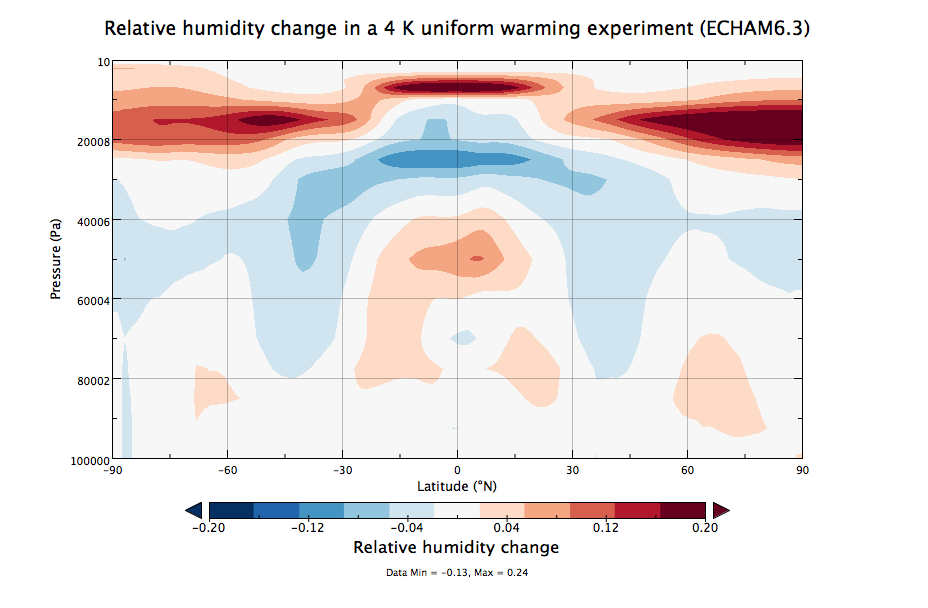
\includegraphics[width=14 cm]{../external_figures/RH_change_echam-6_3_02p4_amip4K_zonalmean.png}
\end{center}
\caption{ Change in relative humidity in a model experiment where the ocean surface temperature is raised uniformly by 4 K.} 
\label{fig:RH_change_ECHAM}
\end{figure}

Fortunately, we can argue that relative humidity ($RH$) stays approximately constant under climate change. Relative humidity is the actual water vapor pressure ($e$) relative to the saturation vapor pressure ($e_s$). For the argument we will be making it is perhaps easier to think of the water vapor mixing ratio which is conserved with adiabatic motion ($q$, such that $RH \approx q/q_s$). If we trace an isolated air parcel along it's trajectory through the atmosphere we will find that it spends part of its time being saturated within clouds and part of its time being sub-saturated in clear air. As long as it is inside clouds it will have $q=q_s$, and so too at the exact moment the parcel leaves the cloud. Let us call this $q_s(T_c)$ where $T_c$ is the temperature at the last contact with cloud. Subsequently, in the cloud-free part of the parcels trajectory, where by necessity $T \ge T_c$, the water vapor mixing ratio at the last contact with cloud is conserved and so the relative humidity is $RH = q_s(T_c)/q_s(T) \le 1$. 

We can think of the total atmospheric circulation as consisting of many such trajectories of small parcels of air, each undergoing cloudy and cloud-free transects. Now, suppose the atmospheric circulation stays unchanged in a statistical sense under small amounts of climate change, then the only thing that changes for our parcels is the temperatures at which they operate. If then the entire troposphere warms at about the same rate, then for a given trajectory both $T_c$ and $T$ change by the same amount and so to first order $RH$ stays constant under climate change. To investigate how good an approximation this is, I plotted the change in $RH$ in Figure \ref{fig:RH_change_ECHAM} as the difference between two experiments: one with sea-surface temperatures prescribed as observed and one wherein I added a horizontally uniform warming of 4 K. In most of the troposphere the changes in $RH$ is less than or around 1 percent per Kelvin warming. In the tropopause and lower stratosphere region there is a substantial rise in $RH$, in part associated with a rise of the tropopause as discussed in the first chapter.

With this result at hand we can now estimate how the specific humidity changes with warming. Our starting point is the Clausius-Clapeyron relation for the saturation vapor pressure:
\[ \frac{de_s}{dT} = \frac{L}{R_v T^2} e_s, \]
which can be rewritten as:
\begin{equation}
\frac{d\ln e_s}{dT} = \frac{L}{R_v T^2},
\label{eq:clausius_clapeyron}
\end{equation}
such that the fractional rate of change of the saturation vapor pressure is a simple function of temperature. $L$ denotes the latent heat of evaporation (about $2.5 \cdot 10^6$ J kg$^{-1}$) and $R_v$ is the gas constant for water vapor (about $461$ J kg$^{-1}$ K$^{-1}$). Inserting different temperatures on the right hand side of Equation \ref{eq:clausius_clapeyron}, one finds that near the Earth's surface one finds increases of 6-8 percent per degree warming, and for tropical upper-tropospheric temperatures around 14 percent per degree warming. Since most of the water vapor resides in the lower troposphere the water vapor path scales with close to 7 percent per degree warming.

The reader is reminded that the infrared part of the water vapor feedback only works because the atmosphere is colder than the surface. Thus adding a water vapor molecule to the atmosphere near the surface is less effective than adding it near the tropopause, and so despite the amount of water vapor in the upper troposphere is much smaller than near the surface it still plays an important role in controlling the infrared radiation to space. The troposphere is colder than the surface in most places and at most times. 
An exception where the atmosphere can be warmer than the surface occurs at high latitudes in winter, and so there raising the emissivity of the atmosphere by adding water vapor will result in more infrared radiation escaping to space. 
It is left as an exercise to estimate the infrared part of the water vapor feedback under the assumption of constant relative humidity using the MODTRAN model and compare the result with that of more complex climate models. 

A not negligible part of the water vapor feedback of about 20-30 percent, however, occurs because water vapor absorbs sunlight. This absorption depends less on where in the vertical the water vapor is, and more on the column integrated amount, the latitude and season, as well as the presence of clouds and the reflectivity of the surface.

% Show a figure with Clausius-Clapeyron, argue that the warming of parcels moving from the upper troposphere to the lower is larger in a warmer climate, hence a slight reduction in RH

\subsection{Cloud feedbacks}
\label{sec:cloud_feedback}
Clouds are exceptionally complicated, and it would be foolish to even try to account for the many different ways in which clouds could possibly feed back on the Earth's energy balance. And not only are the mechanisms complex and difficult to grasp, they are also the main source of uncertainty in quantifying climate change and clouds impact the strength of other feedback mechanisms as we have seen above in the example of surface albedo feedback. Therefore, cloud feedbacks are very much central to the part of climate sciences that aims at estimating Earth's climate sensitivity. Because it is so complicated, one current trend is to dissect the cloud feedback into separate regimes (Figure \ref{fig:cloud_feedback_illustration}) wherein the hope is that the individual mechanisms can be understood and quantified. It is not at all clear that this is the most effective way to achieve overall progress, though, and climate scientists also pursue other routes to determining cloud feedback. 
Current thinking is that it is useful to divide cloud feedback into three groups:
\begin{itemize}
\item Mid- to high latitude mixed-phase clouds
\item Low-level clouds 
\item Deep clouds
\end{itemize}
although one could certainly think of other divisions that would be meaningful. The first two categories act mostly in the shortwave bands by regulating the planetary albedo, whereas the third category is thought to mainly function in the longwave by regulating the infrared radiation emitted to space.

\begin{figure}
\begin{center}
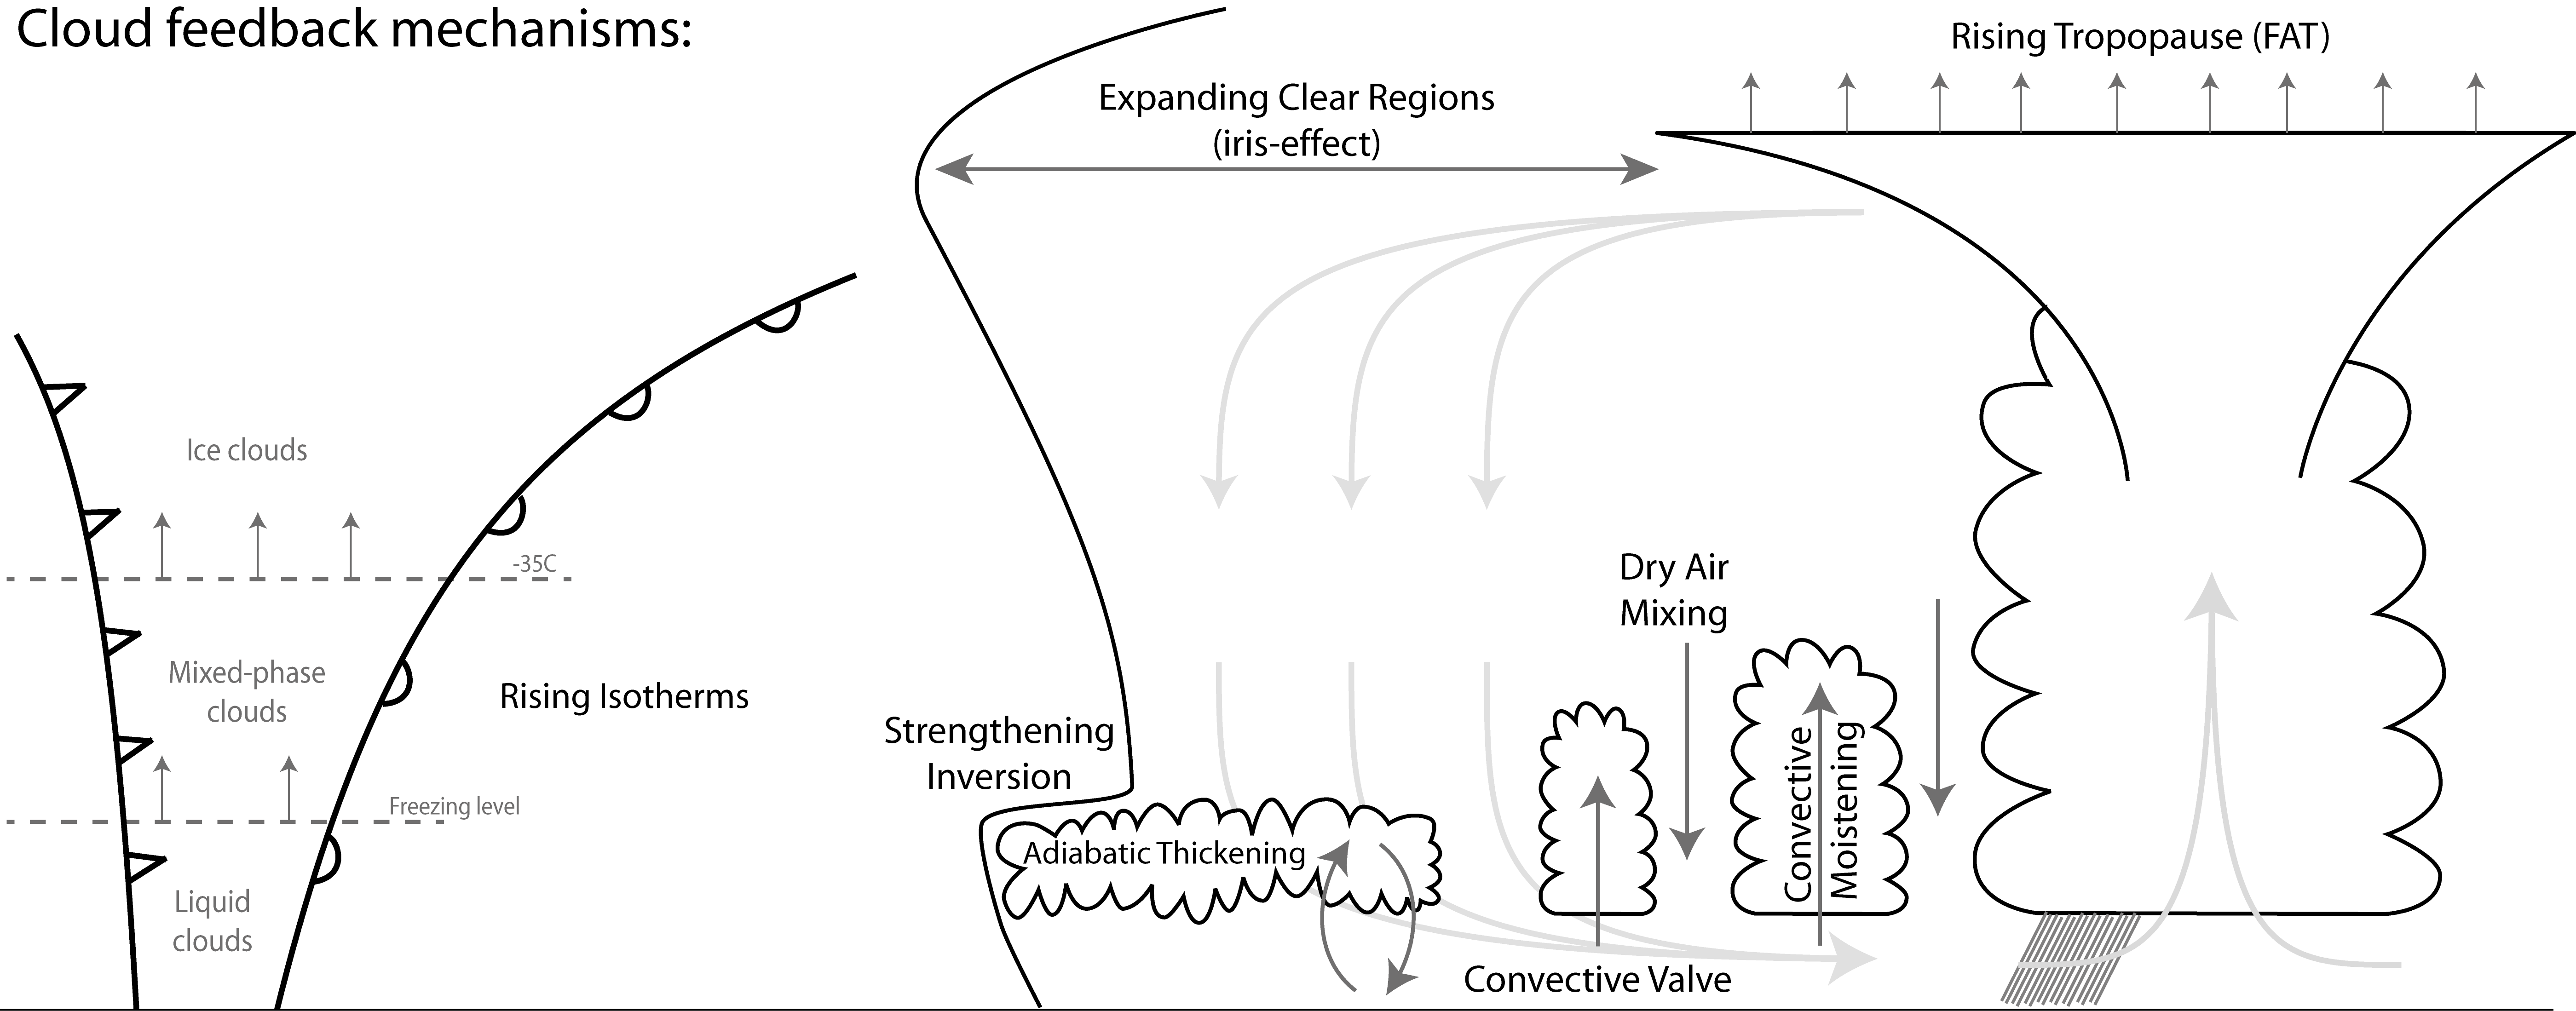
\includegraphics[width=17 cm]{../illustrations/Cloud_feedbacks_illustration.png}
\end{center}
\caption{ Illustration of various cloud feedback mechanisms. To the left is mixed-phase cloud feedback occurring at mid- to high latitudes in for instance frontal clouds, in the lower middle I show several mechanisms related to low-level stratocumulus and trade-wind cumulus cloud feedbacks, and to the right are deep cloud feedbacks which are thought to act mainly by regulating the infrared radiation escaping to space. } 
\label{fig:cloud_feedback_illustration}
\end{figure}

\subsubsection{Mixed-phase clouds}
Ice clouds are generally less reflective to sunlight than are liquid clouds. This is primarily because ice crystals tend to be few and large, whereas cloud droplets tend to be small but many: the cross-section of many small droplets is larger for a given amount of condensate. In a warming climate the isotherms will move upward in the atmosphere and poleward alone resulting in a larger fraction of liquid clouds (Figure \ref{fig:cloud_feedback_illustration}), and so a negative shortwave cloud feedback must result. 

If all clouds at temperatures below the melting point (0$^\circ$C), then a very strong negative feedback would result. However, it is a bit more complicated. At temperatures above 0$^\circ$C all clouds consist of the liquid phase, and below about -35$^\circ$C all clouds consist of ice phase. Between these temperatures both phases can exist, we say clouds are of mixed phase. The more one can maintain liquid clouds at temperatures below the melting point, the weaker the mixed-phase feedback is as there is simply less ice clouds that can be transformed.

Signs of what might be dominating negative mixed-phase cloud feedback can be seen in the Southern Ocean, North Pacific and the Arctic in the MPI-ESM-LR model (Figure \ref{fig:feedback_maps}). This is not the only type of cloud feedback in those regions though, and for instance total cloud feedback appears to be positive in the North Atlantic, a region where we would also expect mixed-phase cloud feedback to be active. A couple of recent studies try to observationally constrain mixed-phase feedback. One study finds that complex climate models are on average correct, with some models having stronger and some models having weaker feedback. Another study finds that models as a whole overestimate the strength of the negative mixed-phase cloud feedback, implying that models overly dampen global warming.

\subsubsection{Low-level clouds}
Low-level clouds in the tropics and sub-tropics on the contrary consist mostly of liquid droplets. They are, nevertheless, consistently identified as the main source of spread in complex climate model feedback, which is likely due to there being a large number of competing mechanisms (Figure \ref{fig:cloud_feedback_illustration}), explaining all of which I couldn't possibly do any justice here. Foremost, the low-level clouds may regulate the planetary albedo either by changing their coverage or by changing their reflectivity. The reflectivity of low-level clouds is mainly controlled by the amount of condensate. We saw previously that in a warmer climate the atmosphere holds more water vapor, as of Clausius-Clapeyron, and so a naive expectation is that low-level clouds will thicken as there is more vapor to condense (adiabatic thickening). Counteracting this, is the mixing of the moist lower atmospheric air with dry air subsiding from aloft: in a warmer climate the difference in specific humidity will be larger between the boundary layer and the subsiding air, and so the mixing down of air (top entrainment) results in a larger depression of relative humidity and fewer clouds in a warmer climate. The strength of the mixing, in turn, is controlled by the strength of the temperature inversion above the boundary layer. In some regions of the sub-tropics this inversion is expected to strengthen in a warmer climate resulting in more cloudiness. Overall, complex climate models can exhibit both positive and negative low-level cloud feedbacks, but there is a tendency for observational and fine-scale cloud modeling evidence to favor positive feedback from this regime.

\begin{figure}
\begin{center}
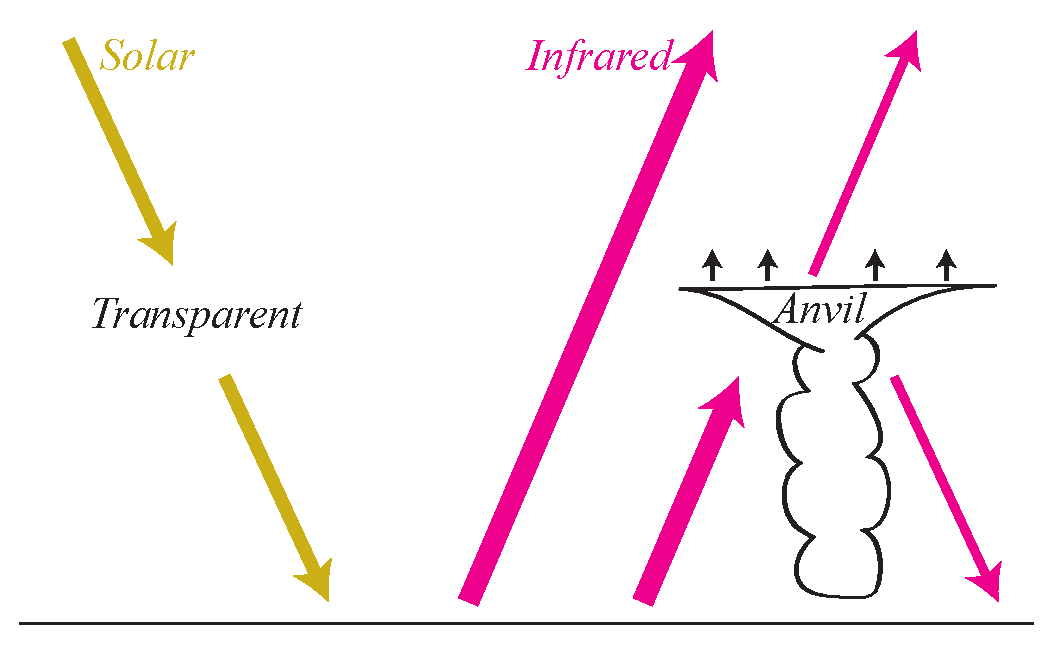
\includegraphics[width=10 cm]{../illustrations/Deep_cloud_feedback_illustration.pdf}
\end{center}
\caption{ Illustration of the infrared feedback from deep clouds. The upper level clouds are thought to move upward in a warming climate so as to maintain a nearly constant temperature of about 200 K, alone resulting in the positive fixed-anvil temperature feedback. There may also be changes in the anvil coverage, something which is popularly denoted iris-effect. } 
\label{fig:deep_cloud_feedback_illustration}
\end{figure}

\subsubsection{Deep clouds}
Deep cloud feedbacks originate for the most part in the tropical regions. We argued in an earlier chapter that the tropopause might move upward in a warming climate so as to maintain an approximately constant temperature, and with it, presumably also that of the deepest convective cloud tops (anvils). 
To see how this ascendence of upper level clouds might exert a cloud feedback, let us consider the gray body case with an upper-level cloud that covers a fraction, $f$, which acts as an ideal black body. The cloud is assumed to rise such as to maintain a constant temperature with a warming surface temperature ($dT_a/dT_s=0$, Figure \ref{fig:deep_cloud_feedback_illustration}). Since there is only one unknown in our problem, $T_s$, we also only need to form one energy balance equation; we choose the top of the atmosphere:
\begin{equation}
N = \frac{S_o}{4}(1-\alpha) - (1-f) \epsilon \sigma T_s^4 - f\sigma T_a^4.
\label{eq:anvil_balance}
\end{equation}
First, let us assume that $f$ is constant such that the upper level cloud maintains its coverage, then we can calculate the feedback parameter:
\begin{equation}
\lambda =  - 4(1-f) \epsilon \sigma T_s^3,
\end{equation}
where we remember that $dT_a/dT_s=0$. Comparing to the Planck feedback parameter, Equation�(\ref{eq:lambda_planck}), we immediately recognize that this can be rewritten as:
\begin{equation}
\lambda =  \lambda_P + f 4 \epsilon \sigma T_s^3,
\end{equation}
where the second term is then the fixed anvil temperature (FAT) feedback parameter. Notice how the actual temperature of the cloud, $T_a$, plays no role in determining the strength of the feedback. Since the FAT feedback parameter equals $-f\lambda_P$ we can readily estimate what $f$ has to be around 0.11 to provide the longwave cloud feedback parameter found in complex climate models ($\lambda_{C,LW}$, Table \ref{table:feedbacks}). The estimate of $f$ is smaller than expected since tropical upper-level cirrus clouds cover a larger fraction of the Earth, perhaps twice as much. However, because they consist of few relatively large ice crystal their longwave emissivity is usually less than unity and so in this more realistic setting it requires a larger coverage to reach the same amount of feedback. Additionally, deep clouds often occur in regions where there is also abundant water vapor, and thus the planetary emissivity ($\epsilon$) lower, also resulting in the required $f$ to be larger.

Now, let the area $f$ covered with our upper-level black body cloud vary with temperature to emulate an iris-effect. Now the derivative with respect to $T_s$ of Equation (\ref{eq:anvil_balance}) becomes a bit more complicated:
\begin{eqnarray}
\lambda &=&  \lambda_P + f 4 \epsilon \sigma T_s^3 + \epsilon \sigma T_s^4\frac{df}{dT_s} - \sigma T_a^4\frac{df}{dT_s} \nonumber \\
&=&  \lambda_P + \lambda_{FAT} +  \sigma \left( \epsilon T_s^4 - T_a^4\right)\frac{df}{dT_s},
\label{eq:lambda_iris}
\end{eqnarray}
where we recognize the second term as the FAT feedback parameter. The third term represents a replacement of radiation originating from the upper-level cloud to radiation originating from the surface if $df/dT_s$ is negative. In this extreme example it takes only a 2 percent per degree warming reduction of the anvil coverage ($df/dT_s \approx -0.02f$) for the iris-effect feedback parameter to be as strong as  $\lambda_{FAT}$. This is an underestimate of the amount of reduction required for several reasons. First, if cloud cover decreases then the planetary albedo also decreases, thereby inducing a compensating positive shortwave cloud feedback. Second, most of the upper-level cirrus cloud is optically too thin to act as ideal black bodies, further requiring a larger reduction. Together, I believe it might take around 5 percent reduction per degree warming, or so, to be able to compensate the positive FAT feedback.
Complex climate models exhibit no, or only very weak, reductions of anvil area with warming, whereas different lines of observational evidence suggest that models underestimate this reduction. The interpretation of the data, however, remains contentious and it is also currently not known mechanistically why anvil coverage would reduce substantially in a warming climate.

% Add a figure with Earth's effective emissivity from CERES, also clear sky
% Use this to argue that $f$ is larger because the local \epsilon is much smaller in the deep tropics were convective cloud feedbacks act



\newpage
\vspace{1 cm}
{\setlength{\parindent}{0cm}
%\hrule
\begin{exercise}
Estimate the limit of instability for planetary albedo feedbacks using equation \ref{eq:lambda_general}.  Assume here that $\epsilon$ is a constant. Put in numbers relevant for Earth to estimate how fast planetary albedo would have to decrease to alone cause instability.  
\end{exercise}

\begin{exercise}
Calculate the feedback parameter $\lambda = dN/dT_s$ for the partially absorbing slab atmosphere derived in the previous chapter, section \ref{sec:partially_absorbing_slab}. Do so by eliminating $T_a$ from the top-of-atmosphere imbalance equation and then take the derivative with respect to $T_s$. Calculate ECS with reasonable parameters for Earth.
\end{exercise}

\begin{exercise}
Use the online MODTRAN radiative transfer model to estimate water vapor feedback. Do so by changing the 'Water Vapor Scale' from, say, 1.00 to 1.07, corresponding to a 7 percent increase of specific humidity which is roughly what occurs for a 1 K warming at typical tropospheric temperatures. Another way to do this is to use the 'Ground T offset', which actually increases the temperature of the whole column, then compare the cases with constant vapor pressure and relative humidity. It is convenient to use the 'Save this run to background' button.
How does the water vapor feedback depend on locality? How does your estimate compare with that of complex climate models?
\end{exercise}

\begin{exercise}
Estimate the ECS using the complex climate model ensemble mean feedback factors $ \lambda_P + \lambda_{W+LR} + \lambda_C + \lambda_A$ as listed in Table�$\ $�\ref{table:feedbacks}. Note that you are to use the sum of the water vapor and lapse-rate feedbacks. What happens to ECS if each feedback is one standard deviation larger, respectively, smaller? Repeat the calculations without cloud feedback. 
\end{exercise}

}


%---------------------------------------------------------------------
\chapter{Temporal evolution}
\label{chapter:evolution}
In the previous chapter we focussed on the stability of stationary states and the equilibrium response to a small forcing. Here we will investigate how the system approaches these equilibria and how it responds to forcing. This involves considerations of the relevant heat reservoirs, and ignorance of those that do not matter. On this background we will develop a mixed-layer and a two-layer model and study their behavior. 

\section{Heat capacities}
When we think of the Earth's climate system there are several components that can absorb energy with different heat capacities and with different timescales involved. Usually we think of the oceans as the largest component followed by the atmosphere and cryosphere. There are, however, parts of these components that are closely connected to the surface temperature, and there are parts that are weakly connected to the surface. This means, foremost, that it is meaningful to divide the oceans into two or more parts.

If we start with the atmosphere, we saw in the first chapter how the troposphere is for the most part quickly stirred, mixed or overturned by various motion. Therefore it does not take very long for air to be mixed around the world, roughly on the order of months, though the time it takes to cross the equator can be longer. The stratosphere in turn, we found was in radiative equilibrium and stably stratified; though it isn't motionless. There are quite strong zonal winds, and also there is an overturning circulation called the Brewer-Dobson circulation. The latter starts at the tropical tropopause with upward motion, goes up, poleward and terminates in the high latitudes. It takes, however, on the order of five years. The atmosphere weighs in at nearly 10.000 kg m$^{-2}$, which corresponds to the hydrostatic surface pressure of 98.500 Pa, or about that of a column of 10 meters of liquid water. The specific heat capacity of air is, however, a factor four less than for water (Table \ref{table:capacity}) and so in terms of total heat capacity the atmosphere is equivalent to 2.5 meters of water per unit area. The troposphere is close to 90 percent of the atmospheric mass, and so it is reasonable to disregard the upper atmosphere here. 

There is only a tiny fraction of water vapor in the atmosphere, about 25 kg m$^{-2}$, which corresponds to 2.5 cm if it was all condensed and distributed onto the surface. But the energy it takes to evaporate a kilogram of water is substantial, $L \approx $  2.500.000 J kg$^{-1}$. In the previous chapter we learned that relative humidity stays roughly constant under climate change and that this results in roughly a 7 percent increase in specific humidity per degree warming. Converting this latent heat into an equivalent heat capacity we find that the energy storage due to evaporation of water vapor corresponds to about 1.0 meters of water per unit area.

The oceans are on average about 4 km deep and cover about 70 percent of the earth's surface -- a massive heat reservoir compared to the equivalent heat capacities for the atmosphere derived above. However, only the uppermost part of it called the mixed-layer is in immediate contact with the surface. The layer is mixed by turbulent motion mostly caused by atmospheric winds exerting stress at the ocean surface and is typically 50-100 meters deep. Thus, this mixed-layer alone is much larger than the atmospheric heat capacity which we estimated above to be approximately the equivalent of 2.5 plus 1.0 m of water. The rest of the ocean mixes more slowly and it is thought that a full overturning of the ocean will take several millennia. The slow mixing into the deeper oceans happens across a continuum of scales, first into the thermocline ($\approx$ 500 m) and then into the deep ocean via complex circulations. For the purpose of this course, however, we shall model the heat capacity of the mixed-layer (plus atmosphere) and deep oceans as only two separate components. 

The cryosphere can be considered a kind of (anti) heat reservoir. Just opposite to water vapor in the atmosphere, which is a higher energetic state than liquid water, ice is a lower energetic state: melting ice requires energy and it takes about 338.000 J kg$^{-1}$. The cryosphere on Earth is dominated by the two large ice-sheets in Antarctica ($26\cdot10^6$ km$^3$) and Greenland ($2.8\cdot10^6$ km$^3$), whereas for comparison the Arctic sea ice is two to three orders of magnitude less abundant ($20\cdot10^3$ km$^3$). But where sea ice responds relatively quickly to the surface temperature with a timescale of a few years, the ice sheets can take several millennia to adjust to a new climate. The time it would take for glaciers to melt is uncertain, but for the considerations here we can safely neglect the cryosphere.

But how about the Earth's soils and crust? There is substantially more mass there than in any of the above compartments. Well, fluctuations in surface temperature do propagate downward in the soils and rock, albeit at a very slow rate. Under typical conditions it takes 100 years for a perturbation at the surface to be felt at all at 150 m depth, and a 1.000 years to reach 500 m depth; a fact that one can use to reconstruct temperatures in past centuries by measuring temperatures in boreholes. This propagation is so slow because the thermal conductivity of soils and bedrock is low compared to that of a moving fluid or gas, typically by many orders of magnitude. Therefore, even though the soil and crust have similar specific heat capacities to air (Table \ref{table:capacity}) and represent an enormous mass, it plays only a minor role in determining the flows of energy in the Earth system; one that we shall neglect here.

\begin{table}
  \caption{ Specific heat capacities and some thermal conductivities. For water and air the thermal conductivity is dominated by turbulent or advective motion. }
  \vspace{0.5 cm}
  \centering
  \begin{tabular}{l|rr}
%    \hline
      & Heat capacity (J kg$^{-1}$ K$^{-1}$) &  Conductivity (W m$^{-1}$ K$^{-1}$) \\
    \hline
    Water              & 4,181 &         {\em flow-dependent}   \\
    Air                   & 1,004 &         {\em flow-dependent}    \\
    Soil                 & 800 & 0.5-1.5           \\
    Granite           & 790 & 1.7-4.0             \\
  \end{tabular}
  \label{table:capacity}
\end{table}

It is upon this rather elaborate background that we shall treat the heat capacities of the Earth in the following as consisting of two components: 1) the troposphere plus ocean mixed-layer as representative of the global mean surface temperature ($T$), and 2) the deep oceans with a separate temperature ($T_d$). This turns out to be a surprisingly good approximation to much more complicated climate models.


\section{The mixed-layer model}
Let us first assume the simplest case where the whole system is represented by a single heat capacity, $C$. We may here think of the uppermost part of the ocean and the atmosphere; a model we refer to as the mixed-layer model simply because as of the above argumentation the upper ocean heat capacity is at least an order of magnitude larger than the rest. The mixed-layer model is the basis for our further considerations and the concept is widely used. In the mixed-layer case with a single heat capacity the imbalance results in a temperature change, such that:
\begin{equation}
N = C\frac{dT}{dt}. 
\label{eq:mlo_imbalance}
\end{equation}
We can next assume small perturbations around some stationary state, $T_o$, such that $T$ is no longer the absolute temperature but rather the temperature relative to $T_o$:
\begin{equation}
C\frac{dT}{dt} = F + \lambda T,
\label{eq:mlo}
\end{equation}
where $F$ is some external forcing. 

Let us first consider a system at a stationary state, whereat at time $t=0$ we abruptly apply a constant forcing $F$, forever. We can realize that this is a solution to the differential equation:
\begin{equation}
T(t) = \frac{-F}{\lambda}\left(1-e^{\frac{\lambda}{C}t}\right),
\label{eq:mlo_solution}
\end{equation}
which can be verified by inserting equation \ref{eq:mlo_solution} into equation \ref{eq:mlo}. We readily recognize the equilibrium response by inserting $t=\infty$ such that the expression in parentheses is unity:
\begin{equation}
T(\infty)=\frac{-F}{\lambda},
\label{eq:mlo_equilibrium}
\end{equation}
which clearly reminds us of the special case for a doubling of CO$_2$, $ECS=-F_{2x}/\lambda$, developed in an earlier chapter. It is perhaps worth noting here that the equilibrium response is not dependent on how one got there since there is only one unique solution as long as $\lambda < 0$ everywhere. In deriving our solution we assumed that the full forcing was applied instantaneously and held constant forever, but we could also imagine ramping up (or down) forcing over a finite period of time and then holding it constant; the end result will be the same.

\begin{figure}
\begin{center}
\includegraphics[width=12 cm]{../plots/Mixed_layer_temperature_abrupt_forcing.pdf}
\end{center}
\caption{ Numerical solutions to equation \ref{eq:mlo} to an abrupt forcing of $F_{2x}$ with varying values of $ECS$ of 1, 2, 3, 4, and 5 K. The heat capacity is chosen to correspond to that of an ocean covering the entire surface of the Earth with a depth of 50 m which is a typical equivalent depth found in complex climate models. The dashed line shows the initial slope and the dots shows the e-folding response at time $\tau$. } 
\label{fig:mlo_plot}
\end{figure}

Next, let us look at the temporal behavior of the mixed-layer ocean. First, let us look at the initial warming rate of the system by evaluating the time-derivative of our solution at time $t=0$:
$$\frac{dT}{dt}\Bigr|_{t=0} = \frac{F}{C},$$
which is simply the rate of energy input ($F$) divided by the heat capacity. The initial slope is completely independent of the feedback parameter, and hence the climate sensitivity, of our model. To demonstrate this, I plot solutions with widely varying $\lambda$ in Figure \ref{fig:mlo_plot} and the analytical initial slope. It turns out that in the first few years the actual solution stays close to the initial slope and only after some time do climate change feedbacks begin to affect the solution. This has important consequences for attempts to estimate Earth's climate sensitivity from short term forcing from volcanoes.

For intermediate time-scales we may consider the time it takes to obtain some fraction of the equilibrium response. Here it is common to define the e-folding time as the time it takes for the response to reach $1-e^{-1}$, or roughly two thirds, of the equilibrium ($e\approx 2.718$). Remembering that $\lambda<0$ to obtain stable solutions, we may define the response time:
$$\tau \equiv \frac{-C}{\lambda}$$
which depends on the heat capacity and the feedback parameter, and not the forcing. Inserting this into equation \ref{eq:mlo_solution}, and substitute in equation \ref{eq:mlo_equilibrium}, we obtain a different form of the solution:
$$T(t) = T(\infty)\left(1-e^{-\frac{t}{\tau}}\right)$$ 
such that when $t=\tau$ the system has reached a fraction $1-e^{-1}$ of the equilibrium. From this we can readily realize that the more sensitive the system is, the longer it takes to reach equilibrium. In Figure  \ref{fig:mlo_plot} I plotted the response time which increase from roughly 2 to 10 years for $ECS$ from 1 to 5 K. The slower equilibration of the more sensitive models is readily visible: after about 10 years the low sensitivity models have practically reached equilibrium, but the high sensitivity models continue to warm.

Another interesting type of forcing is a fast injection or release of energy. We might think of the forcing as represented by  Dirac's delta function, but the main point is that it should be active only for a short period of time compared to the response time of the system. A volcanic eruption could be considered such a case with reasonable approximation. Whatever the reason, though, the result is that at time $t=0$ we might find the system out of equilibrium such that $T(0) \ne 0$ and subsequently we can set $F=0$. The solution to this is, as was also the case for the abrupt forcing, an exponential function:
\begin{eqnarray}
T(t) &=& T(0)\cdot e^{\frac{\lambda}{C}t} \\
       &=& T(0)\cdot e^{-\frac{t}{\tau}} \nonumber
\end{eqnarray}
but where we previously started with $T(0)=0$ we now have the system approaching the equilibrium state $T(\infty)=0$. Notice how for the mixed-layer ocean that the e-folding time, $\tau$, to a delta forcing is the same as that for the abrupt forcing.


% Include a case of a delta-forcing? 
% T(t)=T(0)*e{\frac{\lambda}{C}t}

\subsection{Numerical solutions}
The mixed-layer model can be readily solved analytically for the case of an abrupt forcing and doing so has several advantages. But as we add complexity to our model and might want to consider noise or forcing that varies in time the analytical solution quickly becomes intractable. Therefore we shall often resort to a numerical solution. The equations we want to solve are generally quite simple such that the first-order Euler time-stepping method can be used. We can approximate:
$$ \frac{dT}{dt} \approx \frac{\Delta T}{\Delta t}, $$
where the large $\Delta$ indicate finite changes in temperature and time, rather than infinitesimal, such that we might think of $\Delta T = T(t+\Delta t)-T(t)$. Inserting this into equation \ref{eq:mlo} and rearranging:
\begin{equation}
T(t+\Delta t) = T(t) + \frac{\Delta t}{C} \left[F(t)+\lambda \cdot T(t)\right], 
\label{eq:numerical_solution}
\end{equation}
where we have defined the right hand side of equation \ref{eq:mlo} to be evaluated at time $t$, and the forcing to be a function of time. The equation can then be solved by stepping forward in a time-loop. To yield sufficiently accurate results we need to make small enough time steps: for our purposes we will be making monthly steps.  It is left as an exercise to test this approximation.
In Python the time integration can be programmed as a for-loop and might look something like this:
\begin{verbatim}
   for t in range(0,nstep-1):
        T_ml[t+1] = T_ml[t] + delta_time/C_ml*(forcing[t]+lambda_0*T_ml[t])
        imbalance[t+1] = C_ml*(T_ml[t+1]-T_ml[t])/delta_time
\end{verbatim}
where we recognize the terms in equations \ref{eq:mlo_imbalance} and \ref{eq:numerical_solution}. The code can readily be extended to solving more complex differential equations that we shall derive later.

Although we shall not use the following methodology during this course, for completeness  of presentation I want to mention that there is an elegant way to solve the evolution of a linear climate system to a time-varying forcing. Here it is assumed that a general evolving forcing $F(t)$ can be considered to consist of an additive sequence of many small abrupt forcings, or 'steps'. If, for instance, the surface temperature response to forcing $F_{2x}$ from a doubling if CO$_2$ is $R(t)$ (see Figure \ref{fig:mlo_plot}) then we can estimate the surface temperature evolution as a sum of the response to all previous steps up until the time $t$:
$$ T(t) \approx \sum_{i=0}^{t-1} \frac{R(t-i)}{F_{2x}}\cdot \left[F(i)-F(i-1)\right], $$
where the quantity in brackets is the incremental forcing change. The step-response method is particularly useful in that the response function $R$ can also be derived from complex climate models by conducting a single abrupt forcing experiment. Further, one can think of the response function in more general terms to mean anything that varies in time after an abrupt forcing is applied such as local temperature, or even the hydrological cycle, so that we are not limited to think of the global mean surface temperature. The method, however, assumes linearity in that each step solution is independent of the others. In a later chapter we shall introduce non-linearity which will prohibit us from using the step-response method.


\section{The two-layer model}
Although the mixed-layer model is attractive in its simplicity, for the timescales we are interested in however, the vast heat capacity of the deep ocean plays an important role. We may readily extend the mixed-layer model to a two-layer model by adding an additional heat reservoir of the deep ocean, $C_d$. The imbalance of the system can then be calculated as the sum of the rate of change of heat in the two reservoirs:
\begin{equation}
N = C\frac{dT}{dt} + C_d\frac{dT_d}{dt}, 
\label{eq:twolayer-imbalance}
\end{equation}
where $T_d$ is the deep ocean temperature. In this simplest form, it is assumed that the deep ocean is not in direct contact with the surface and so does neither feel directly the atmospheric feedbacks nor the radiative forcing. It is connected to the mixed-layer by diffusive and/or advective processes such that at some set of states $(T, T_d)$ the net flux is zero; we shall take these to be $T=T_d$. Note that the temperature of the real world deep ocean ($\approx 3^\circ$C) is colder than that of the surface because deep water formation occurs primarily in polar regions; the temperatures in the two-layer model $(T, T_d)$ are to be thought of as relative. We shall further assume the flux is proportional to the difference, such that:
\begin{equation}
C_d\frac{dT_d}{dt} = \gamma(T-T_d), 
\label{eq:twolayer-deep}
\end{equation}
where $\gamma$ is the deep ocean heat uptake efficiency which has values on the order of 1 Wm$^{-2}$K$^{-1}$. Whenever the mixed-layer is warmer than the deep ocean heat will flow to reduce the difference and vice-versa. In order to conserve energy, i.e. satisfy equation \ref{eq:twolayer-imbalance}, we must amend the mixed-layer by subtracting the flux into the deep ocean:
\begin{equation}
C\frac{dT}{dt} = F + \lambda T - \gamma(T-T_d).
\label{eq:twolayer-ml}
\end{equation}
The resulting set of coupled differential equations \ref{eq:twolayer-deep} and \ref{eq:twolayer-ml} is the two-layer model. It is helpful to realize that if you insert \ref{eq:twolayer-deep} and \ref{eq:twolayer-ml} into equation \ref{eq:twolayer-imbalance} you get:
$$N = F + \lambda T,$$
that is, the imbalance of the two-layer model is determined solely by the mixed-layer temperature and the external forcing. The deep ocean is here only 'felt' at the top-of-the-atmosphere through the moderation of the mixed-layer temperature. We shall later return to a case wherein the deep ocean temperature is allowed to affect the radiation balance.

\begin{figure}
\begin{center}
\includegraphics[width=17 cm]{../plots/Two_layer_temperature_abrupt_forcing.pdf}
\end{center}
\caption{ Numerical solutions to the two-layer model (blue) equations \ref{eq:twolayer-deep} and \ref{eq:twolayer-ml} to an abrupt doubling of CO$_2$ with an $ECS$ of 2.77 K. Light blue dots are results from MPI-ESM1.2 which has the same ECS. Shown in black is the mixed-layer model, and the gray dashed line is the initial slope. } 
\label{fig:two_layer_plot}
\end{figure}

Let us first look at the behavior of the two-layer model starting at rest with $T=T_d=0$ and we apply an abrupt forcing, $F$, at time $t=0$ and then keep it constant forever. Since the imbalance is purely determined by the mixed-layer temperature only, we immediately obtain that the longterm equilibrium response is the same as before:
$$ T(\infty)=\frac{-F}{\lambda}.$$
Likewise, the initial warming rate is determined only by the heat capacity of the mixed-layer, since at time $t=0$ the ocean heat uptake into the deep ocean is zero:
$$\frac{dT}{dt}\Bigr|_{t=0} = \frac{F}{C}.$$
Thus, when exerted to an abrupt forcing both the longterm response and the initial slope is the shared between the mixed-layer and two-layer models.

It is when we consider the intermediate timescales of decades to centuries that the mixed-layer and two-layer models behave differently. For the mixed-layer model we were able to derive an exact analytical solution and saw that it behaves as an exponential relaxation towards the equilibrium. It is also possible to derive an exact analytical solutions to the two-layer model, as shown for instance by Geoffroy et al.\cite{geoffroy2013a}, but this is far too complicated for this course and further obtaining the exact solution provides little physical insight. In broad terms, though, we can think of the deep ocean as introducing a slow time-scale, $\tau_d$ which is of the order of centuries, such that the solution is approximately the weighted sum of two exponentials $T(t) \approx \frac{-F}{\lambda}(1-a e^{\frac{-t}{\tau}}-b e^{\frac{-t}{\tau_d}})$, where $a+b=1$. 

Instead, I solve the two-layer model numerically as shown in Figure \ref{fig:two_layer_plot} where I also compare it to the mixed-layer model and the results from a complex climate model, MPI-ESM1.2. We see that the overall behavior of MPI-ESM1.2 is captured well by the two-layer model; a fact that makes the two-layer model a particularly useful starting point for studies of climate dynamics. There are two small differences, though: in the first few years MPI-ESM1.2 warms faster most likely because it also includes some land which has a low heat capacity, and on decadal timescales the warming in MPI-ESM1.2 is a bit slower. 

A caveat with the two-layer model is that the single deep-ocean temperature is to represent a diverse set of mixing- and advective processes that constitute the Earth's deep ocean circulation. Therefore, to get a reasonable match of the two-layer model to more complex models, such as MPI-ESM1.2, we have to use a somewhat smaller heat capacity than that of the full deep ocean of about 4,000 m depth covering some 70 percent of the surface, corresponding to a mean depth of 2,600 m if distributed over the entire Earth's surface. Instead, I use about half of that -- 1,200 m global equivalent -- to compromise between relatively fast mixing into the upper deep ocean and slow mixing deeper down. One can model this with more levels, or a full three dimensional general ocean circulation model, but this comes at the expense of transparency.

Finally, let us take a look at the temperature response of the two-layer model to a delta forcing. Here we imagine that heat is rapidly extracted from- or injected into the mixed-layer such that the deep ocean cannot react, that is, at time $t=0$ we have  $T\ne 0$ and $T_d=0$. If we then evaluate the initial rate of change of the mixed-layer temperature (\ref{eq:twolayer-ml}) then we obtain:
\begin{equation}
\frac{dT}{dt}\Bigr|_{t=0} = \frac{T(0)}{C}\left[\lambda - \gamma\right],
\end{equation}
yielding the result that the deep ocean heat uptake acts to restore the surface temperature faster towards it's original state. Remember that $\lambda$ is likely somewhere in the range -1 to -2 Wm$^{-2}$K$^{-1}$, and so the effect of $\gamma$ is to nearly double the restoration rate relative to that of the mixed-layer model: if the delta forcing was for instance due to a volcanic eruption that lead to a cooling of the mixed-layer, then the deep ocean will transfer heat towards the surface thereby warming the mixed-layer up again. It is left as exercises to explore this case.

\begin{figure}
\begin{center}
\includegraphics[width=12 cm]{../plots/Zero-layer-model_rampup.pdf}
\end{center}
\caption{ Comparison of the two-layer model (solid curves) to the zero-layer model (dashed lines). The colors indicate the speed of the ramp-up of the forcing: Blue corresponds to 1 percent CO$_2$ concentration increase per year, whereas green is 2 percent, and red is 4 percent increase per year. Marked is also the warming at year 70 in the first experiment which is defined as the transient climate response (TCR).} 
\label{fig:zero_layer_plot}
\end{figure}

\section{The zero-layer model}
\label{sec:zero-layer}
An approximate diagnostic version of the two-layer model can be obtained for the case of a gradually changing forcing. We will use the fact that the mixed-layer and the deep ocean heat capacities are distinctly different by more than an order of magnitude. Thus, there must be some intermediate timescales that are long enough so that the mixed-layer heat capacity can be ignored ($C\rightarrow 0$) and still short enough that the deep ocean warming can be ignored ($C_d \rightarrow \infty$). In this limit, the two-layer model surface temperature (equation \ref{eq:twolayer-ml}) simplifies to:
\begin{equation}
0 = F + \left(\lambda - \gamma \right)T,
\label{eq:zero-layer}
\end{equation}
and from equations \ref{eq:twolayer-imbalance} and \ref{eq:twolayer-deep} we get $N=\gamma T$. Thus, the evolution of the surface temperature is purely a function of the forcing:
$$T(t)=\frac{F(t)}{\gamma-\lambda}.$$
We call this the zero-layer approximation as there are no layers left that have memory and the result is a purely diagnostic equation relating temperature, forcing and imbalance with bulk properties of the system. I plotted both the zero- and the two-layer models exposed to forcing that increases linearly in time in Figure \ref{fig:zero_layer_plot}. We usually think of experiments with, say, a 1 percent increase in atmospheric CO$_2$ per year, yielding a doubling of the concentration in about 70 years -- this corresponds roughly to the anthropogenic forcing increase since the 1950's. The temperature response after 70 years in this experiment is often referred to as the transient climate response (TCR). Because the forcing is logarithmic in the CO$_2$ concentration this corresponds to a nearly linear increase in time. The zero-layer approximation works surprisingly well on multi-decadal timescales for these types of forcing that changes gradually. In the first decades the zero-layer model overestimates warming as the mixed-layer heat capacity still matters, whereas after about 70 years the model underestimates surface warming as the deep ocean begins to warm up. Further, the faster we increase the forcing the more the zero-layer model overestimates the initial warming.
The zero-layer model is being extensively used to interpret the instrumental record warming in terms of inferring Earth's climate sensitivity; a theme that we shall return to later.




%\section{Sea-level rise}
%About 3 mm year$^{-1}$.


\newpage
\vspace{1 cm}
{\setlength{\parindent}{0cm}
%\hrule
\begin{exercise}
Observations suggest that Greenland currently looses around 200 km$^3$ ice per year (1 km$^3$ = 10$^9$ m$^3$). Estimate a) the part of Earth's energy imbalance that goes into the current melting of the Greenland ice sheet, b) how much it contributes to global sea level rise in millimeters per year, and c) how long it will take until Greenland is gone if melt continues at the current pace? Remember the surface area of the Earth is 510$\cdot$10$^{12}$ m$^2$, the oceans cover about 70 percent of the surface, and that the density of ice is about 900 kg m$^{-3}$. 
\end{exercise}

\begin{exercise}
Verify that the numerical solution of the mixed-layer model yields a close approximation to the exact solution in equation \ref{eq:mlo_solution}. You can conveniently download the simple mixed-layer model written in Python from my web page. To evaluate the exponential function in the analytical solution you can use Numpy's version, np.exp(), which accepts an array as input, e.g.
\begin{verbatim}
np.exp(lambda_0/C_ml*time)
\end{verbatim}
The script contains two commented out lines (starting with \#) towards the end that you can use as a starting point. What happens if you choose a longer time-step length, e.g. a year?
\end{exercise}

\begin{exercise}
Imagine the Earth is hit by an asteroid. The impact whirls debris into the atmosphere which results in a temporary rise of the planetary albedo and hence a surface cooling. The debris is relatively heavy and therefore falls out of the atmosphere within weeks of the impact such that we can consider the asteroid impact a delta forcing. The rapid cooling leaves the system shortly after the impact at $T(0)=-6.0$ K. We shall assume the Earth has an $ECS=3.0$ K and a mixed-layer heat capacity  corresponding to a global mean depth of 50 meters: $C= 50\cdot 1000 \cdot 4181$ J m$^{-2}$K$^{-1}$. 
If you ignore the deep ocean, how many years would it take until the mixed-layer temperature reaches $T=-1.0$ K?
If you consider a deep ocean, which is roughly unaffected directly during the asteroid impact such the $T_d(0)=0$, would the surface temperature reach $T=-1.0$ K faster or slower?
\end{exercise}

\begin{exercise}
Solve the asteroid impact exercise numerically for the two-layer model and compare with the mixed-layer model. You can conveniently use the two-layer model programmed as a Python function that you can download from my web page. The script will as default run five abrupt CO$_2$ doubling experiments with different ECS and plot them. Remove those experiments, set the input\_forcing to zero at all times and set the mixed-layer initial temperature as desired in the call to the function 'twolayermodel' (T\_ml0 = -6.0). The two-layer model can be tricked to be a mixed-layer model by setting gamma=0.0 in the function call: 
\begin{verbatim}
exp_mixlayer = twolayermodel(forcing_years, input_forcing, T_ml0=-6.0, gamma=0.0)
exp_twolayer = twolayermodel(forcing_years, input_forcing, T_ml0=-6.0)
\end{verbatim}
Plot the result and verify your inference from the previous exercise.
\end{exercise}

}

%---------------------------------------------------------------------
\chapter{External forcing and fast adjustments}
\label{chapter:forcing}
The climate system can be forced in a number of ways, and previously we have taken the concept of external forcing from a doubling of atmospheric CO$_2$ for granted. But what we mean by external forcing is not always obvious. The first thing we need to do is to define the system we are looking at. Often we think of the physical properties of the system: the temperature, humidity, clouds and surface albedo, whereas other components such as the solar constant or the atmospheric CO$_2$ are considered as "given" external boundary conditions. Feedbacks are then those internal processes within the system that respond to changes in the external boundary conditions in ways that achieves a new balanced climate. 

But even some of those internal processes may not respond in concert with the surface temperature: we have already looked at the sluggish deep ocean in the previous chapter, but also ice sheets may take millennia to equilibrate with a new climate, and vegetation may react to changes in boundary conditions such as CO$_2$ or sunlight over long timescales. In a later chapter we shall develop a way to handle the possible impact of the slow deep ocean adjustment process as a time-dependent feedback. 
Also at short timescales -- and this is what we shall investigate here -- things can change in ways that do not depend directly on the temperature. We shall see below how the stratosphere cools off rapidly, within weeks, after an increase in CO$_2$ which is a consequence of the increased emissivity allowing it to cool more effectively. But also clouds may respond to atmospheric composition changes in multiple ways, actually within seconds to hours, well before the global mean surface temperature has had time to respond.

\vspace{0.5 cm}
\noindent
When trying to separate {\bf feedback} from {\bf forcing} I find it useful to think of the responses that impact the radiation balance as to whether, or not, they depend physically on the surface temperature. For instance, the increase in water vapor depends mostly on the temperature, hence it is a feedback, but in other cases it may not be so straightforward. Therefore we often resort to a more ad-hoc definition by dividing the problem into time-scales. We call things that happen well within the first year after a forcing is applied {\bf fast adjustments} and those that happen in congruence with surface temperature we define as {\bf feedbacks}. Finally, those that involve long timescales are often referred to as {\bf slow- or time-dependent} feedbacks. It is, however, often quite challenging to separate these effects. 
%A clear short-coming of this division occurs for vegetation which may respond to purely the CO$_2$ fertilization, but over long timescales. 

\section{Solar forcing}
To be a little more concrete, let's take the perhaps simplest case of an abrupt but small change in the solar constant, $\delta S_o$. We may now perturb our energy balance equation \ref{eq:black_body_energy_balance} for the black body Earth and assume the planetary albedo stays constant:
$$ N+\delta N \approx \frac{S_o+\delta S_o}{4}(1-\alpha) - \sigma (T_e+\delta T)^4 $$
Now, the system was in balance before the abrupt change, so $N=0$, and initially as the change in solar constant is applied we still have $\delta T=0$, such that we can estimate the change in the radiation balance induced by the change in solar constant:
$$ \delta N(t=0) \approx \frac{\delta S_o}{4}(1-\alpha).$$
We can think of this initial change in the radiation balance as the forcing, $F$. Traditionally, climate modelers apply a 2 percent increase in the solar constant, giving $F_{2pct}\approx 4.8$ Wm$^{-2}$ which is close to that of a doubling of CO$_2$, $F_{2x}\approx 3.7$ Wm$^{-2}$. 

We may, however, imagine things could happen on a short timescale that are not congruent with the surface temperature response to the solar forcing. The first is that some of the extra sunlight will be absorbed by ozone in the stratosphere, and because the stratosphere has a low heat capacity and is not dynamically coupled to the surface it can quickly warm up. The warmer stratosphere will radiate more infrared radiation both down towards the surface and up to space, the latter resulting in a weakening of $F_{2pct}$ by some small amount. 

Second, clouds could respond to the stronger solar input thereby altering the planetary albedo. From our everyday experience it seems plausible that cloudiness is tied to sunlight: fair weather cumulus clouds form in summer over land in the afternoon, deep convective thunderstorms occasionally in the late afternoon or evening. But perhaps more significant here, low-level stratiform clouds (fog, stratus, stratocumulus) tend to thin or dissipate when exposed to sunlight. 
Such  changes in cloudiness can result in an adjustment term $-\delta \alpha \cdot S_o/4$, or 3.4 Wm$^{-2}$ per percent change in $\alpha$. Thus, even minute changes in $\alpha$ can have substantial impacts on the adjusted $F_{2pct}$.

\vspace{0.5 cm}
\noindent
In the following we shall go over two methods to estimate forcing, and then take a closer look at the forcing from CO$_2$. There are of course many other ways the Earth system can be forced, some of which we shall look at in a later chapter in the context of historical warming. 

\section{The Gregory- and the Hansen methods}
There are many ways to estimate the radiative forcing in climate models. Here I will go over the two practical methods that are most widely used today namely those suggested by Gregory et al. (2004) and Hansen et al. (2005). Both methods build on the idea of the linear framework we developed earlier wherein the energy balance is a function of forcing and feedback:
$$N=F+\lambda T$$
where $F$ and $\lambda$ are assumed to be constants. 

The Gregory-method builds on coupled climate simulations wherein CO$_2$, or any other forcing for that matter, is abruptly applied whereafter the system slowly warms. Then the parameters $F$ and $\lambda$ can be determined by linear regression of $N$ versus $T$. The best way to see this is to plot yearly mean values of the imbalance as a function of global mean surface temperature change (Figure \ref{fig:gregory_hansen}). Note that in the figure I show a case with quadrupled CO$_2$, or two doublings, rather than the usual single doubling of CO$_2$. The radiative forcing from CO$_2$ is roughly logarithmic in the concentration (Arrhenius 1896) and so if we divide the forcing estimate by two we get an estimate of that from a single doubling. Using 4xCO$_2$, rather than 2xCO$_2$, is popular in the climate modeling community as it increases the ratio of the forced signal over internal variability (noise) when trying to fit simple models to the results, such as we do here. By applying a larger forcing, however, we also risk activating non-linearities that again makes interpretation more difficult.

\begin{figure}[!]
\begin{center}
\includegraphics[width=10 cm]{../plots/MPI-ESM12_abrupt4xCO2.pdf}
\end{center}
\caption{ Imbalance versus global mean surface temperature following an abrupt quadrupling of CO$_2$ in the coupled climate model MPI-ESM1.2. Each black dot is an annual average and displayed are the first 300 years of the simulation.  The gray solid line is a linear fit to all 300 years and the gray dashed line is a linear fit to the first 10 years of the simulation. The red dot is the effect of quadrupling CO$_2$ in 30-year long simulations for the period 1979-2008 with the atmosphere-only ECHAM6.3 model wherein the sea surface temperatures are held fixed at their observed values. The red line is an extrapolation back to zero following the Hansen et al. (2005) method. } 
\label{fig:gregory_hansen}
\end{figure}

As we expect for the system to be stable (Chapter 3) the slope of the linear fit is negative; we can identify the slope as the feedback parameter, $\lambda \approx -1.2$ Wm$^{-2}$K$^{-1}$. The intercept with the y-axis, i.e. where $T=0$ can then be interpreted as the forcing, $F$. With this method we find an estimate of $F_{4x} \approx 7.34$ Wm$^{-2}$, corresponding to $F_{2x} \approx 3.67$ Wm$^{-2}$ which is not far from our canonical value of 3.7 Wm$^{-2}$. This apparent agreement, as it shall turn out, is purely coincidental.

Hansen et al. (2005) took a somewhat different approach to estimating forcing in models. They suggested using simulations with atmosphere-only models, wherein the sea surface temperature is held fixed, so as to not allow the system to warm in response to a change in boundary conditions. Often these are referred to as AMIP experiments. One will make two simulations, a control and one with a forcing applied, for instance increased CO$_2$. If $T=0$ we simply have that the forcing equals the change in the radiation imbalance between the two experiments. Unfortunately -- or perhaps fortunately -- the whole Earth is not covered by ocean. The land and sea ice covered regions can change their temperatures in response to the changed atmospheric composition. This alters the global mean surface temperature a little bit, for a quadrupled CO$_2$ concentration approximately by 0.5 K. We can write this as:
$$F = N -\lambda \delta T$$
where $N$ is determined from the difference between the two runs, $\delta T$ is the small change in surface temperature and $\lambda$ is taken to be the longterm average slope as determined using the Gregory-method. In figure \ref{fig:gregory_hansen} I display the Hansen method estimate with the red line, yielding $F_{4x} \approx�9.2$ Wm$^{-2}$, corresponding to $F_{2x} \approx�4.6$ Wm$^{-2}$, or a substantially larger value than found with the Gregory et al. (2004) method.

The two methods can be brought into agreement by relaxing the requirement that $\lambda$ is constant. We note that the first few years the imbalance is somewhat above the longterm mean fitted line. If we fit a line to just the first 10 years we see that the slope is substantially steeper with $\lambda \approx -1.8$ Wm$^{-2}$K$^{-1}$ and has an intercept close to that obtained with the Hansen-method. 
We shall return to the interesting causes and implications of $\lambda$ not being a constant at several later occasions, however, already below we shall see that it has something to do with clouds.

\section{Components of the radiative forcing from CO$_2$}
So far we have focussed on the total forcing from e.g. an increase in the solar constant or the atmospheric CO$_2$, and we have discussed loosely the adjustments that might occur. Here we shall formalize this a bit more by assuming that we  can separate the total imbalance change into contributions from CO$_2$ itself, as well as temperature, water vapor, clouds and surface albedo, and we shall then assume each of them are linear in global mean surface temperature change such that:
\begin{eqnarray}
N &\approx& \sum{ N_i} �   \label{eq:prp} \\
 &\approx&  N_{CO_2} +  N_{T} +  N_{W}  +  N_{C}  +  N_{A}�\nonumber  \\
  &\approx& F^*_{2xCO_2} + F_T  + F_W + F_C + F_A + \left(\lambda_T + \lambda_W + \lambda_C + \lambda_A \right)\cdot T�\nonumber \\
  &=& F_{2x} + \lambda \cdot T \nonumber
%  \label{eq:prp}
\end{eqnarray}
where $F^*_{2xCO_2}$ is the direct radiative flux response to a doubling of CO$_2$ and we have assumed that it does not depend on the temperature. This is not entirely correct, and there are in fact good arguments as to why the direct forcing should increase in a warmer climate. In MPI-ESM1.2 there is a small slope of about 0.03 Wm$^{-2}$K$^{-1}$, that however can safely be neglected for the considerations here.

In Figure \ref{fig:mpi-esm1.2_PRP} I plot all the terms in equation \ref{eq:prp} as well as linear regressions for each term. We see that for all components but clouds, the linear approximation works surprisingly well in this model. Further, for two components, namely surface albedo and water vapor, there is a near-zero y-intercept. This means that these components do not contribute to forcing, but can be considered pure climate change feedbacks. Careful inspection reveals a slightly negative y-intercept for surface albedo, which is due to the fact that it takes 1-2 years for sea ice to melt in response to warming (Block and Mauritsen 2013). 

\begin{figure}
\begin{center}
\includegraphics[width=12 cm]{../plots/MPI-ESM12_abrupt4xCO2_PRP.pdf}
\end{center}
\caption{ Separation of contributions to imbalance as in equation \ref{eq:prp} for the MPI-ESM1.2 coupled climate model run presented in Figure \ref{fig:gregory_hansen}. Solid lines are fitted by linear regression over the full 300 years, whereas the two dashed lines are fitted over the first 10 years of the simulation. The separation is done using so-called partial radiative perturbations (PRP) which involves making multiple radiation calls with state-variables replaced by those from a control simulation. } 
\label{fig:mpi-esm1.2_PRP}
\end{figure}

Non-zero y-intercepts are found for temperature ($F_T$) clouds ($F_C$) and the direct CO$_2$ forcing ($F^*$). In MPI-ESM1.2 roughly half of the total forcing is due to $F^*$ itself, whereas fast temperature and cloud adjustments contribute nearly equal amounts. The direct forcing can be understood from our considerations in Chapter 2 where we argued that increasing the emissivity of the atmosphere reduces the infrared radiation to space because the atmosphere is for the most part colder than the surface. Next, we will try to understand the other two components.

\subsection{Stratospheric adjustment to CO$_2$}
The initial positive contribution to the radiation balance by temperature (Figure \ref{fig:mpi-esm1.2_PRP}) may seem puzzling at first. Actually, the only way this can happen is if a part of the climate system cools in response to the increase in CO$_2$; this happens to be the stratosphere. To show this, I plot global mean temperature profiles from the two simulations with prescribed sea surface temperatures that we used to estimate forcing with the Hansen et al. (2005) method above. We see how the tropospheric temperature is hardly changed, but the stratosphere is around 10-15 K colder in the case with quadrupled CO$_2$ and the stratopause and mesosphere are even colder. 
A cooling stratosphere can also be observed on Earth and in the period of about 1960-2010 it cooled off by about 1.5 K. In the same period CO$_2$ concentration rose from 320 to 390 ppm.


\begin{figure}[!]
\begin{center}
\includegraphics[width=8 cm]{../plots/Stratospheric_adjustment_profiles.pdf}
\end{center}
\caption{ Globally averaged temperature in experiments with prescribed sea surface temperatures. The black is the standard AMIP experiment with ECHAM6.3 for the period 1979-2008, whereas the red profile shows temperatures in an experiment wherein CO$_2$ is quadrupled. These are the same experiments used to estimate forcing with the Hansen method. } 
\label{fig:stratospheric_adjustment_profiles}
\end{figure}

The stratosphere is primarily in a radiative equilibrium between sunlight absorbed by oxygen and ozone and a net heat loss of infrared radiation. The stratosphere receives some infrared radiation from lower levels, but looses more through emission so that the net is negative.
As we saw in Chapter \ref{chapter:essentials} the infrared emissivity of the stratosphere is controlled mostly by CO$_2$, ozone and very small amounts of water vapor. In an exercise we saw how the infrared spectrum changes a bit around the regions where CO$_2$ and ozone are absorbing depending on whether we observe from 70 km or 18 km height, but even so the changes were not dramatic. Already here we can infer that the stratosphere is very far from an ideal black body, $\epsilon_s \ll 1$, as it is transparent to most of the infrared radiation from lower levels. 
As the CO$_2$ concentration is increased the stratospheric emissivity ()$\epsilon_s$) is also increased and so the stratosphere can cool more readily in the infrared. 

\begin{figure}
\begin{center}
\includegraphics[width=12 cm]{../plots/Stratospheric_adjustment_timeseries.pdf}
\end{center}
\caption{ Temporal evolution of the clear-sky flux change after quadrupled CO$_2$ at the top-of-atmosphere and at the 200 hPa level just below the tropopause in the ECHAM6.3 model. The dashed line shows the longterm mean change at the top of the atmosphere. } 
\label{fig:stratospheric_adjustment_timeseries}
\end{figure}

Let us consider the energy balance of the stratosphere approximated by a slab that receives energy from the sun's ultraviolet ($f_{UV}$ is about 2 percent of $S_o$) and from the troposphere that radiates upward as a black body with $T_e\approx$ 255 K, and looses heat by radiating up and down:
$$ N_s = f_{UV}*\frac{S_o}{4} + \epsilon_s \sigma T_e^4 - 2\cdot \epsilon_s \sigma T_s^4 $$
where $T_s$ is a bulk stratospheric temperature. By assuming radiation balance ($N_s=0$) and re-arranging we can estimate the emissivity of the stratosphere:
$$ \epsilon_s = \frac{f_{UV}*\frac{S_o}{4}}{\sigma (T_e^4 - 2 T_s^4)} $$
Taking the temperature at around 35 km height as a bulk representation of the stratosphere we can estimate that under base conditions with $T_s\approx$ 230 K we get  $\epsilon_s \approx$ 0.07 and in order to cool off by 10 K then $\epsilon_s$ has to increase to around 0.20 when we quadruple CO$_2$, something which seems reasonable for an optically thin case where emissivity scales nearly linearly with the number of absorbing molecules. Note that these are merely ballpark estimates, and the real-world situation is of course much more complicated with ozone also adjusting to the changed conditions. 

In our ad-hoc definition of fast adjustments we stated that they should happen well within the first year after a forcing has been applied. Now we can estimate the response time of the stratosphere analogous to that developed in Chapter \ref{chapter:evolution} for the mixed-layer model:
$$\tau_s = -C_s \left( \frac{\partial N_s}{\partial T_s}\right)^{-1}$$
It is left as an exercise to show that the response time after a quadrupling of CO$_2$ is about two weeks.  It is worth noting that the response time is inversely proportional to $\epsilon_s$ and so becomes shorter for higher CO$_2$ concentrations. 

\begin{figure}[!]
\begin{center}
\includegraphics[width=12 cm]{../plots/MPI-ESM12_abrupt4xCO2_PRP_temperatures.pdf}
\end{center}
\caption{ Separation of contributions to imbalance from the components of the temperature response: Planck, lapse-rate and stratosphere as depicted in Figure \ref{fig:planck_LR}. Otherwise as in Figure \ref{fig:mpi-esm1.2_PRP}. The dashed regression line shows the fit to the first 10 years. } 
\label{fig:mpi-esm1.2_PRP_temperatures}
\end{figure}

We can see this process happening in a model in Figure \ref{fig:stratospheric_adjustment_timeseries}. Initially there is more downward flux going out below the stratosphere (200 hPa) than is coming in at the top of the atmosphere. As the stratosphere cools off this radiation deficit is reduced. The flux at 200 hPa is actually quite close to the longterm mean at the top of the atmosphere right from the start. Therefore climate modelers have often in the past used this level to estimate the forcing that will occur after the stratospheric adjustment period. It is, however, problematic to use a fixed pressure level when the tropopause moves up and so nowadays we usually use the Hansen et al. (2005) method to estimate radiative forcing after adjustment. 

In summary, the stratosphere adjusts it's temperature quickly thereby enhancing the radiative forcing from CO$_2$. This fast stratospheric adjustment is the very foundation of the division we made of the total temperature feedback in Chapter \ref{chapter:response} into the tropospheric Planck and lapse-rate feedbacks, and separate out stratospheric adjustment as a forcing (Figure \ref{fig:planck_LR}). We can see how well this works in MPI-ESM1.2 in Figure \ref{fig:mpi-esm1.2_PRP_temperatures} where we see that the stratospheric contribution to the radiation balance has the intercept at around 3 Wm$^{-2}$ and nearly zero slope, i.e. zero feedback parameter. The Planck and lapse-rate components have practically zero y-intercept, and so do not contribute to forcing, but do exhibit substantial slopes and are hence both asserting strong negative feedbacks.


\subsection{Cloud adjustments to CO$_2$}
Less than a decade ago Gregory and Webb (2008) found that, in addition to the stratospheric adjustment, also clouds can add to the forcing through fast adjustment processes; that is, in some respects clouds respond directly to a change in CO$_2$. Before this time climate scientists would run their models to equilibrium and assume that all changes to the clouds were temperature-dependent feedbacks. 

\begin{figure}[!]
\begin{center}
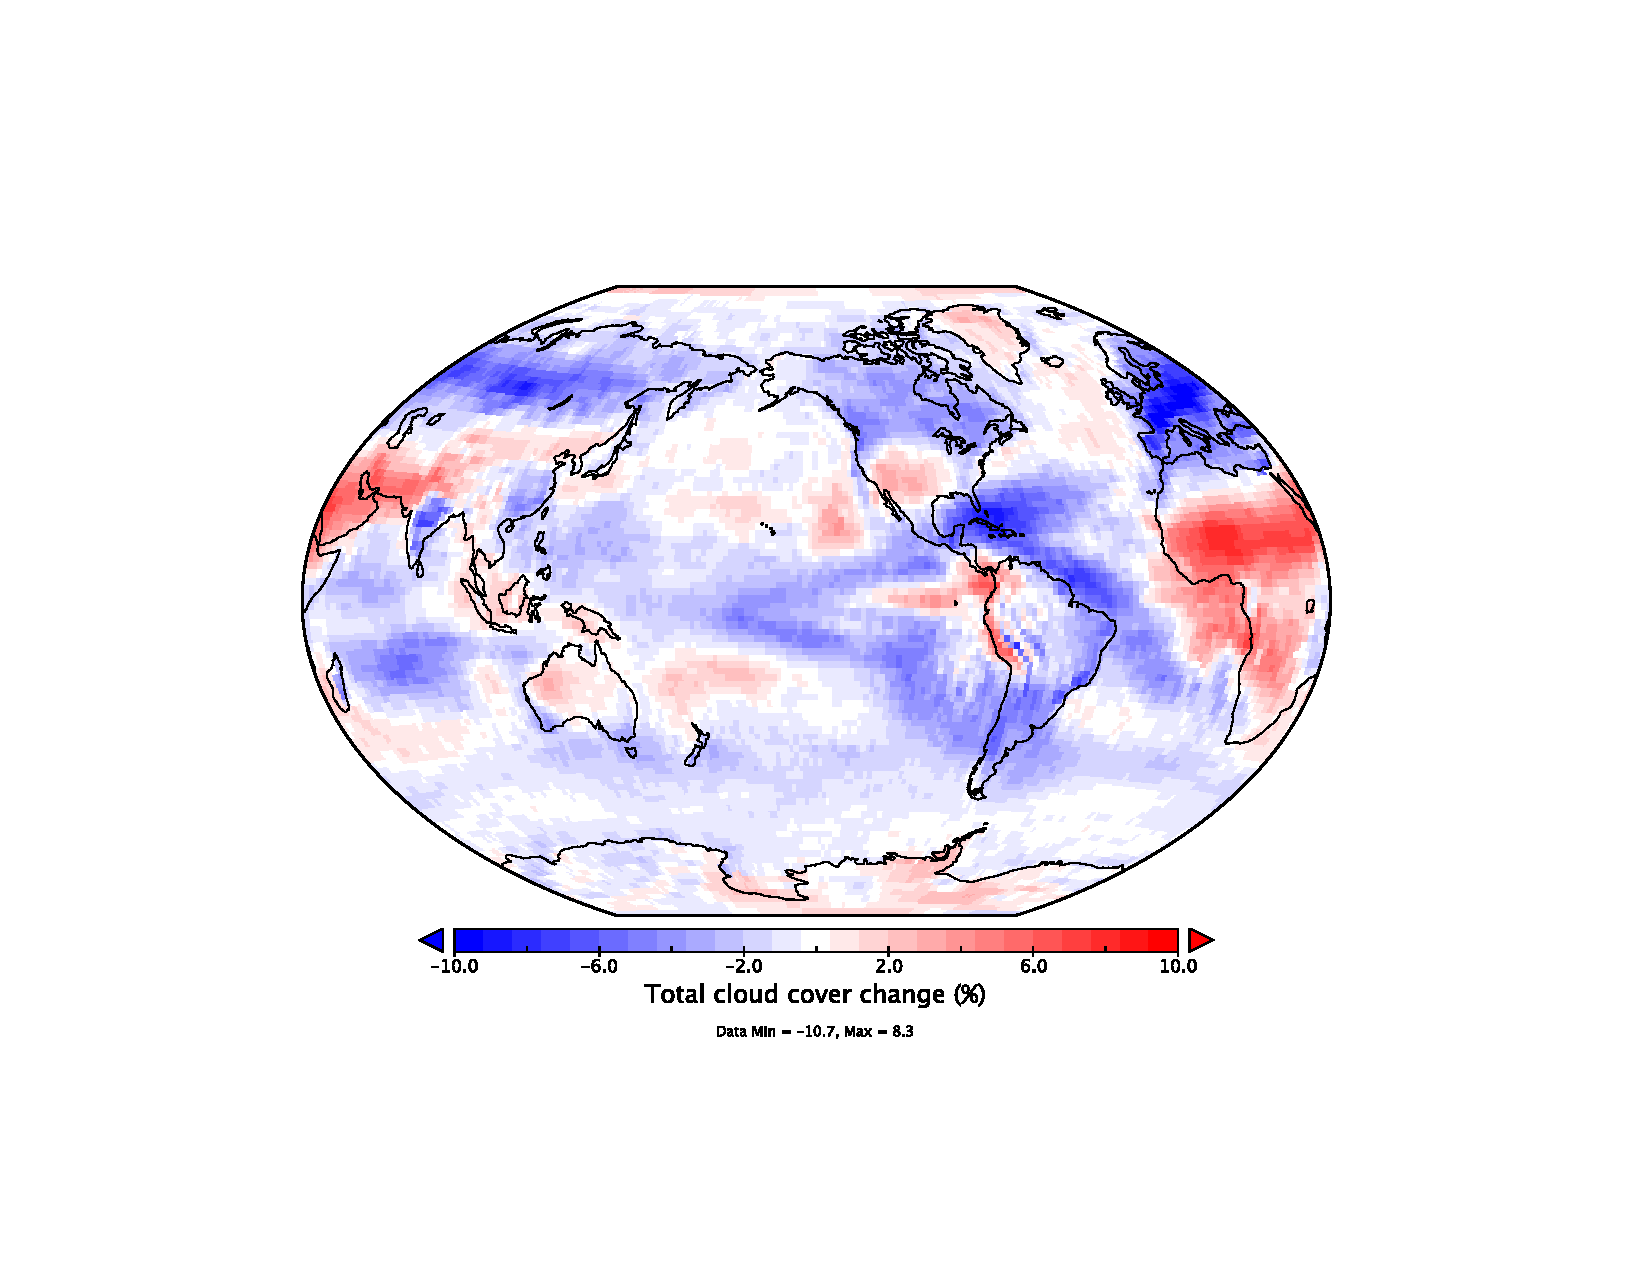
\includegraphics[width=14 cm]{../external_figures/aclcov_BOT_echam-6302p4_amip4xCO2_197.pdf}
\end{center}
\caption{ Cloud cover response to quadrupled CO$_2$ in simulations with ECHAM6.3 and fixed sea surface temperatures for the period 1979-2008. In the global mean the cloud cover is reduced by almost 1 percent. } 
\label{fig:cloud_cover_adjustment}
\end{figure}

We have already seen that in MPI-ESM1.2 -- depending how one counts -- more than half the total change in the radiation balance originating from clouds happens quickly, well within the first year (Figure \ref{fig:mpi-esm1.2_PRP}). We can investigate this fast adjustment using the same experiments that we used in the  Hansen et al. (2005) method. The quadrupled CO$_2$ induces a reduction in global mean total cloud cover of about one percent but large regional deviations occur (Figure \ref{fig:cloud_cover_adjustment}). We see that over most of the oceans, whereat the surface temperature is held fixed, there is a average reduction in cloudiness. Over some land-regions, mostly those associated with monsoons, there is an increase in cloudiness. In the following we shall make qualitative reasoning as to why these two counteracting phenomena occur.

\begin{figure}
\begin{center}
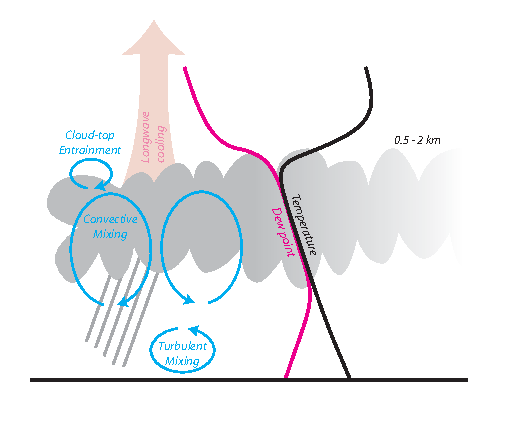
\includegraphics[width=12 cm]{../illustrations/Stratocumulus_dynamics.pdf}
\end{center}
\caption{ Illustration of the key processes involved in low-level stratocumulus clouds: longwave cooling near cloud-top causes condensation and convective instability that drives mixing within the cloud. } 
\label{fig:stratocumulus_dynamics}
\end{figure}

A large class of clouds, in particular over the oceans, are stratiform in nature. The best known is sub-tropical low-level stratocumulus. These are caused by radiative longwave cooling at the cloud-top that cause condensation and convective mixing (Figure \ref{fig:stratocumulus_dynamics}). They mostly occur below a temperature inversion and usually the troposphere above is dry and relatively clear. Under such conditions the cloud-top cooling is particularly strong. In case-studies one can find how stratocumulus thin when a cloud passes by aloft; the upper cloud radiates down towards the stratocumulus thereby reducing the longwave cloud-top cooling. Analogously, low-level stratiform clouds tend to thicken during night and thin or dissipate during day as solar heating counteracts the longwave cooling.

The same phenomenon happens when we increase the atmospheric CO$_2$: the down-welling infrared radiation near cloud top increases due to the higher emissivity of the atmosphere thereby reducing the net cooling. The result is a reduction in this type of clouds within a matter of minutes to hours. From Figure \ref{fig:cloud_cover_adjustment} we infer an order of 1 percent reduction in cloud cover over most of the oceans in response to quadrupled CO$_2$. Assuming a 70 percent ocean coverage, 0.5 local planetary albedo reduction we obtain a cloud adjustment of +1.2 Wm$^{-2}$ to quadrupled CO$_2$, or half of that to a single doubling. This back-of-envelope estimate explains a large part of the difference between the canonical 3.7 Wm$^{-2}$ and the MPI-ESM1.2 models actual forcing of 4.6 Wm$^{-2}$. 

\begin{figure}
\begin{center}
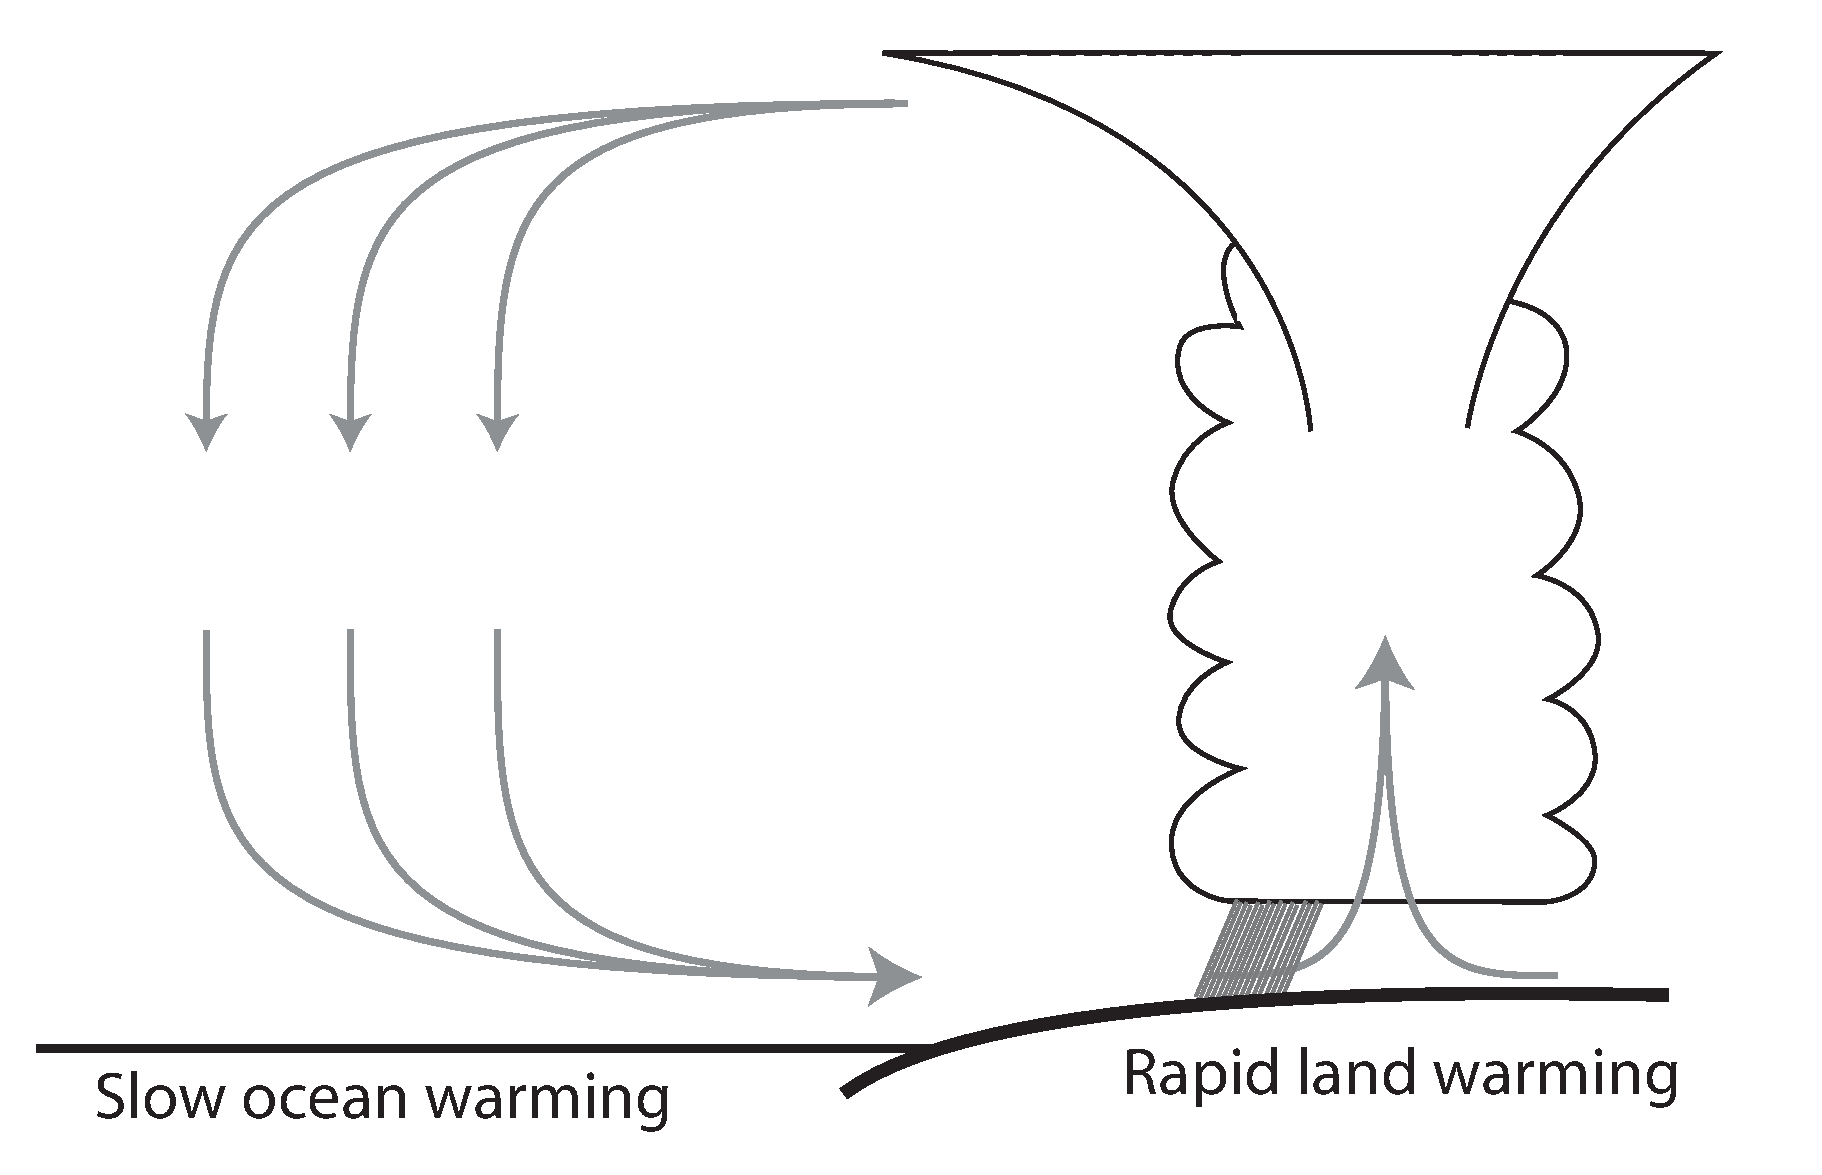
\includegraphics[width=9 cm]{../illustrations/Land_sea_breeze_CO2_illustration.pdf}
\end{center}
\caption{ Illustration of the monsoon-circulation cloud adjustment to increased CO$_2$: an increase in the temperature contrast between land and ocean following an increase in atmospheric CO$_2$ will lead to a direct thermal cell with rising motion over land and subsidence over the oceans. } 
\label{fig:landseabreeze}
\end{figure}

Some tropical land regions see instead increased cloudiness in response increased CO$_2$ in MPI-ESM1.2 (Figure \ref{fig:cloud_cover_adjustment}). They occur over the major monsoon regions, with the notable exception of the Amazon (probably a model bias), ranging from a few up to 10 percent increase in cloud cover over parts of Africa, the Middle East, Australia etc. I believe the reason is that land warms up faster than the ocean (in this simulation the ocean cannot warm), which causes an increased land-sea temperature contrast that drives stronger monsoon circulations (Figure \ref{fig:landseabreeze}). The result is more deep clouds forming over most of tropical lands, in particular upper-level ice clouds. Deep clouds have a near-zero impact on the radiation balance because they both reflect sunlight and at the same time reduce infrared radiation to space.

Cloud adjustments to CO$_2$ are the main source of uncertainty in radiative forcing from CO$_2$. If it wasn't for clouds we would know $F_{2x}$ with very high accuracy, some cite 3.72 Wm$^{-2}$, but clouds introduce model uncertainty of around 20 percent, and MPI-ESM1.2 with its forcing of 4.6 Wm$^{-2}$ is at the upper end when it comes to CO$_2$ forcing.


\section{Aerosol forcings}
Whereas cloud adjustments may play relatively minor roles in determining the forcing from solar constant or CO$_2$ changes, they are decisive in determining the strength of the forcing arising from atmospheric aerosol particles. In fact, there is no shortage of proposed mechanisms in which this may proceed (Figure \ref{fig:ar4aerosols}), as is usually symptomatic when we discuss clouds (Section \ref{sec:cloud_feedback}). 

\begin{figure}
	\begin{center}
		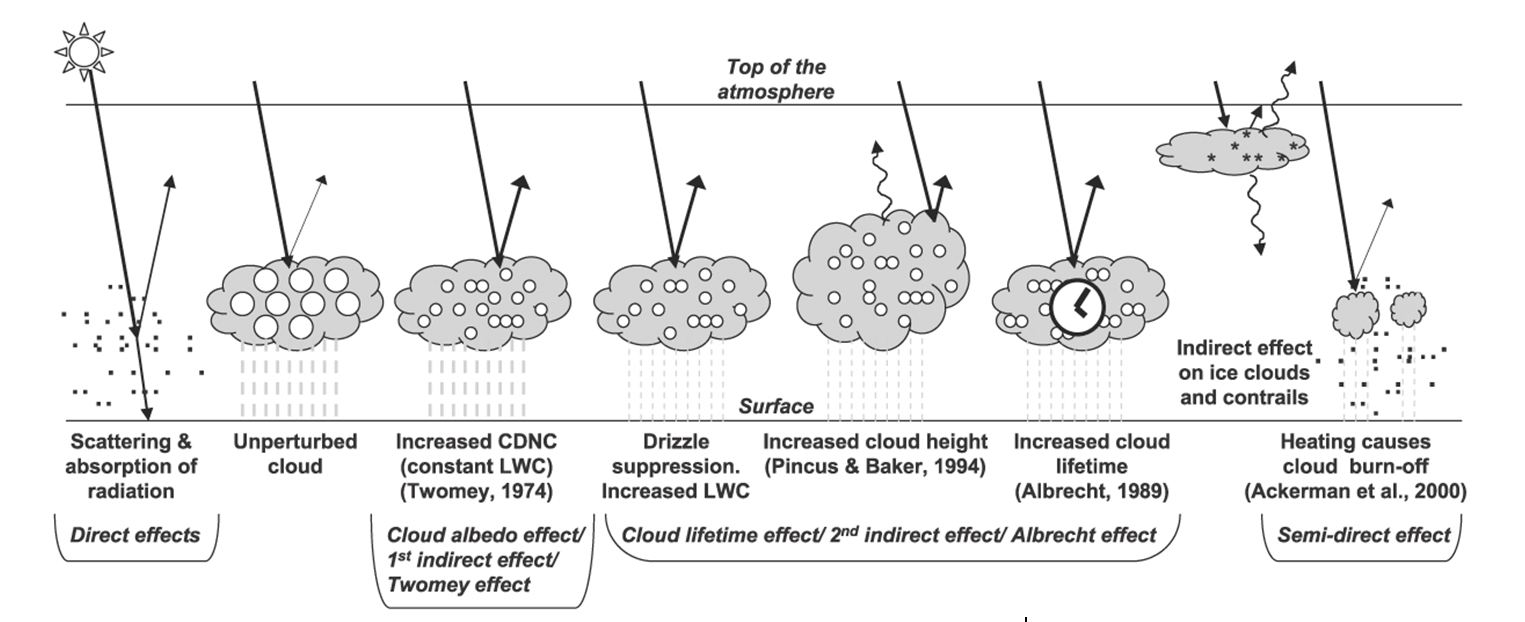
\includegraphics[width=\textwidth]{../external_figures/AR4_aerosol_effects}
	\end{center}
	\caption{ Illustration of different proposed pathways in which aerosol particles may affect the radiation balance. The figure is from the fourth IPCC assessment report. } 
	\label{fig:ar4aerosols}
\end{figure}

Let us however start with the direct impact of aerosols, sometimes referred to as the 'aerosol direct effect' or 'aerosol radiation interactions'. Aerosols can either scatter or absorb sunlight to different degrees depending on their physical properties. By scattering the incoming sunlight that hits the aerosol, photons are sent off course, predominantly in the backwards direction. Therefore, some of the incoming radiation is returned to space, and hence scattering aerosols cool the Earth. Aerosols, may also absorb the photons and thereby warm up the air that surrounds them. To be a positive forcing on the Earth system it is, however, necessary that the photon would have otherwise been reflected to space. Therefore absorbing aerosols that float over dark surfaces, such as the open ocean or dense forests, have nearly no positive forcing. But if above a bright surface such as a snow, ice or deserts, or overlaying a cloud, absorbing aerosols can exert a small positive forcing. Sometimes overlooked, aerosols may further absorb infrared radiation, thus exerting a small greenhouse effect. The total aerosol direct effect caused by human emissions relative to pre-industrial times is thought to be around -0.4 Wm$^{-2}$.

Aerosols are also an important ingredient in clouds; something that you will learn more about in a cloud physics class. In fact, if there were no aerosols around the skies would look very different from what they do today. In order for a cloud droplet to form, it is very helpful to have a particle to start with upon which the water molecules can condense. These are a subset of the aerosol particles that have sufficient size and chemical properties, known as cloud condensation nuclei (CCN). There are typically 10-100 such CCN per cubic centimeter of air, sometimes more in polluted regions, whereas in very clean conditions there can be less than 1. We refer to the impacts of aerosol changes affecting clouds which in turn affect the radiation balance as 'aerosol indirect effects' or 'aerosol-cloud interactions'. 

If we add more CCN to clouds then it is plausible that these clouds will contain more cloud droplets ($N$), in some relation to the increase of CCN, all other things being equal. If the water content in the cloud is the same, i.e. the volume $V=4/3 \pi r^3$, then it must be distributed over more abundant droplets, that as a result will be smaller in size. From a radiation perspective, however, what matters to first order is the cloud droplet cross section area, $A=\pi r^2$, which scale with the square of the droplet radius. We can estimate the relative increase in cross section area between two cases by noting that $V_1=V_2$:
\begin{eqnarray}
\frac{A_2}{A_1} &=& \frac{N_2}{N_1}  \frac{\pi r_2^2}{\pi r_1^2} \nonumber \\
 &=& \frac{N_2}{N_1}  \left( \frac{N_1}{N_2} \right)^\frac{2}{3} \nonumber \\
 &=& \left( \frac{N_2}{N_1} \right)^\frac{1}{3}, \nonumber 
\end{eqnarray}
and thus, the cross-section area is expected to rise slowly with increasing aerosol loading. This is known as the Twomey-effect, and is currently thought to roughly double the aerosol cooling caused by anthropogenic emissions. There is a multitude of additional proposed effects which could both warm and cool the Earth (Figure \ref{fig:ar4aerosols}), but which have fairly little quantitative evidence speaking to them. We shall return to the significance of the associated uncertainty of aerosol forcing as we discuss historical warming.

\newpage
\vspace{1 cm}
{\setlength{\parindent}{0cm}
%\hrule





%\begin{exercise}
%For the system above, estimate how much the planetary albedo, $\alpha$, changes due to clouds adjusting to increased CO$_2$.
%\end{exercise}

\begin{exercise}
Investigate stratospheric adjustment with the MODTRAN model. First calculate the change in the top of atmosphere radiation by quadrupling the CO$_2$ concentration. Then estimate the change near the tropopause. Compare the results with those from ECHAM6.3 displayed in Figure \ref{fig:stratospheric_adjustment_timeseries}. What will happen to the stratosphere?
\end{exercise}

\begin{exercise}
Estimate the response time of the stratosphere after a quadrupling of CO$_2$. You can assume the stratosphere is about 150 hPa thick and so weighs roughly 1500 kg m$^{-2}$, and remember that in the transient you cannot assume $N_s=0$.
\end{exercise}

\begin{exercise}
A climate system has $ECS = 4.5$ K, a non-cloud forcing to a doubling of CO$_2$ of 3.7 Wm$^{-2}$ and a cloud adjustment ($F_C$) of 0.8 Wm$^{-2}$. Calculate the total feedback parameter, and estimate the cloud feedback parameter by assuming the other feedback parameters ($\lambda_P+\lambda_W+\lambda_{LR}+\lambda_A$) are equal to the ensemble mean tabulated in Table \ref{table:feedbacks}. What would the $ECS$ be if the same climate system had fixed clouds?
\end{exercise}

\begin{exercise}
Explain, in your own words, how clouds adjust to an increase in atmospheric CO$_2$.
\end{exercise}

%\begin{exercise}
%Show that the Hansen- and the Gregory methods yield the same forcing estimate if $\lambda$ is constant.
%\end{exercise}


}



%---------------------------------------------------------------------
\chapter{Global variability}
\label{chapter:global_variability}
Variability is everywhere in the quasi-chaos of the Earth's climate system. We can see this variability firsthand in a time series of the observed changes in global mean surface temperature (GMST), as shown in Figure \ref{fig:variability_01}. The evolution of surface warming is, as we can see, not a straightforward increase over time. Volcanoes constantly drive short cooling episodes followed by "rebound" warming, and the time-varying nature of anthropogenic emissions induces wobbles in the warming trend. But if we were to remove the influence of volcanoes, anthropogenic emissions, and other forcings, what would be left behind? 

\begin{figure}
	\begin{center}
		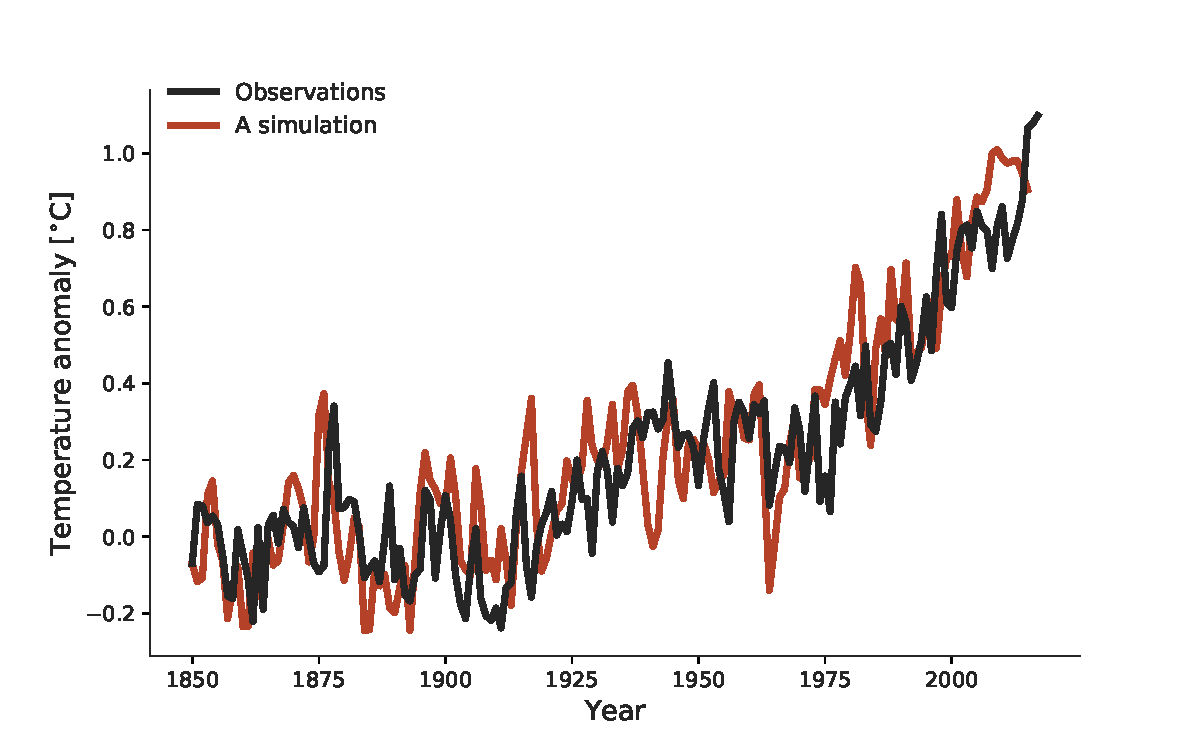
\includegraphics[width=12 cm]{../plots/Variability01.pdf}
	\end{center}
	\caption{ Caption } 
	\label{fig:variability_01}
\end{figure}

We call the naturally-occurring unforced variability in the climate system, \textit{internal variability}, because it refers to internal processes in the system that drive variability even in the unforced climate system. These processes are not completely random (we say ``quasi-chaotic''); they follow well-known oscillatory patterns such as the El-Ni�o Southern Oscillation (ENSO) or the Atlantic Multi-decadal Oscillation (AMO), which are nevertheless difficult to predict. Although internal variability is naturally-occuring, we refer to variability induced by volcanoes and other by non-anthropogenic forcings as \textit{natural variability}. That may be confusing, but it's important to hold the variability relating to forcing separate from the variability inherent in the unforced climate system.

\section{Variability versus forced response}
One reason why this separation is important relates to our expectations of how the climate behaves or \textit{should} behave given an external forcing. If we compare a simulation of climate and the observations of climate, as shown in Figure \ref{fig:variability_01}, there are decade-long periods when the observations and the simulation diverge. Is the model therefore ``wrong'', or are these fluctuations just internal variability?

We can attempt to estimate internal variability in the historical GMST in several ways, including one cutting-edge method that has become possible due to increasing computational power. If we simulate the evolution of temperature on Earth since the pre-industrial era say, 100 times, but introduce small differences into the model's initial conditions, the chaotic nature of the climate system will transform those differences into substantial variations in the GMST: internal variability. If we accept our model as a good-enough representation of the Earth's GMST evolution and the factors that influence it, then each simulation represents how the GMST \textit{might} have behaved in an almost identical world with slightly different initial conditions.

\begin{figure}
	\begin{center}
		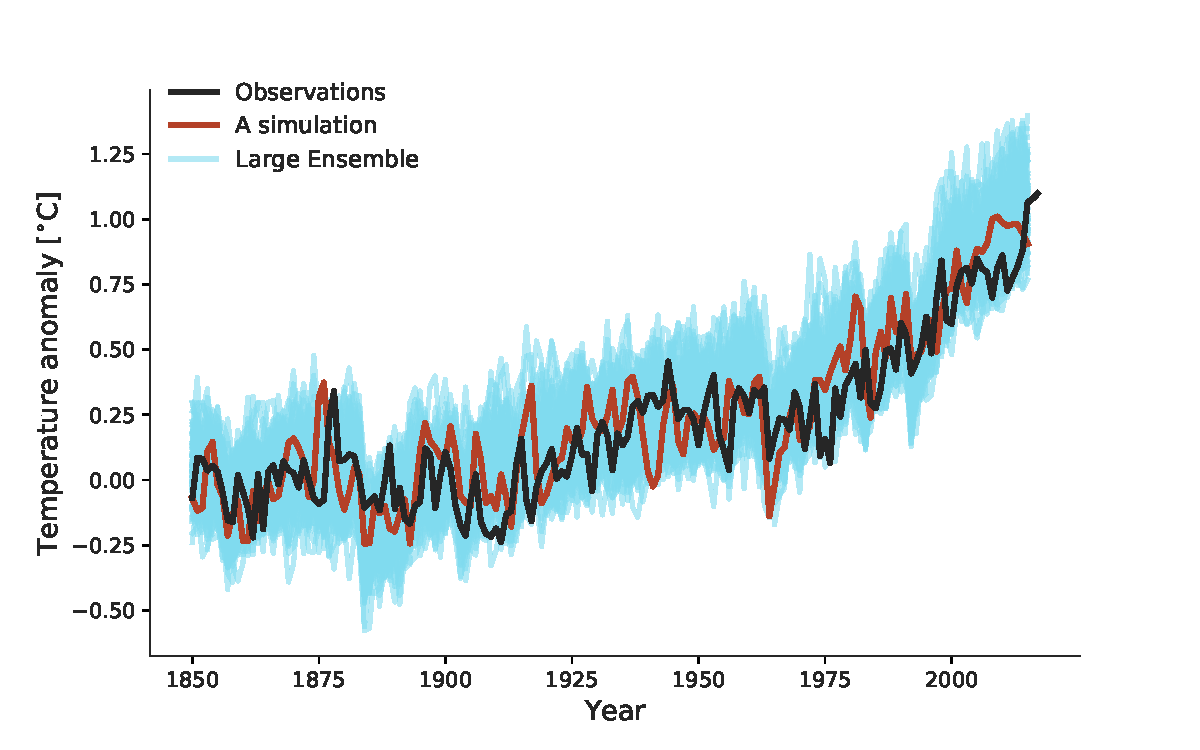
\includegraphics[width=12 cm]{../plots/Variability02.pdf}
	\end{center}
	\caption{ Caption } 
	\label{fig:variability_02}
\end{figure}

In Figure \ref{fig:variability_02} just such an ensemble is depicted, in fact, this is the largest coupled climate model ensemble of the historical period to date: the MPI-ESM grand ensemble. The observations and the single simulation from Figure \ref{fig:variability_01} are also shown, and we see that their deviations lie within the internal variability generated by the ensemble. Both the observations and the single simulation wander up and down, at times amongst the warmest simulations, at times amongst the coolest, but they remain within the bounds of the ensemble.

Because the ensemble is so large, we can even separate the expected forced response from the internal variability. If the distribution in temperature anomalies is Gaussian (it's not but it's very close), then the ensemble mean is an estimator of the true forced response, with a mean standard error that shrinks with ensemble size \textit{n},

\begin{equation}
MSE = E \lbrack \left(  \overline{X} - \mu  \right)^{2}  \rbrack = \frac{\sigma^{2}}{n}.
\label{eq:mse}
\end{equation}

The remaining internal variability in a 100-member ensemble mean is therefore small, leaving the forced response (see Figure \ref{fig:variability_03}), which we can then subtract from every ensemble member to isolate the internal variability.

\begin{figure}
	\begin{center}
		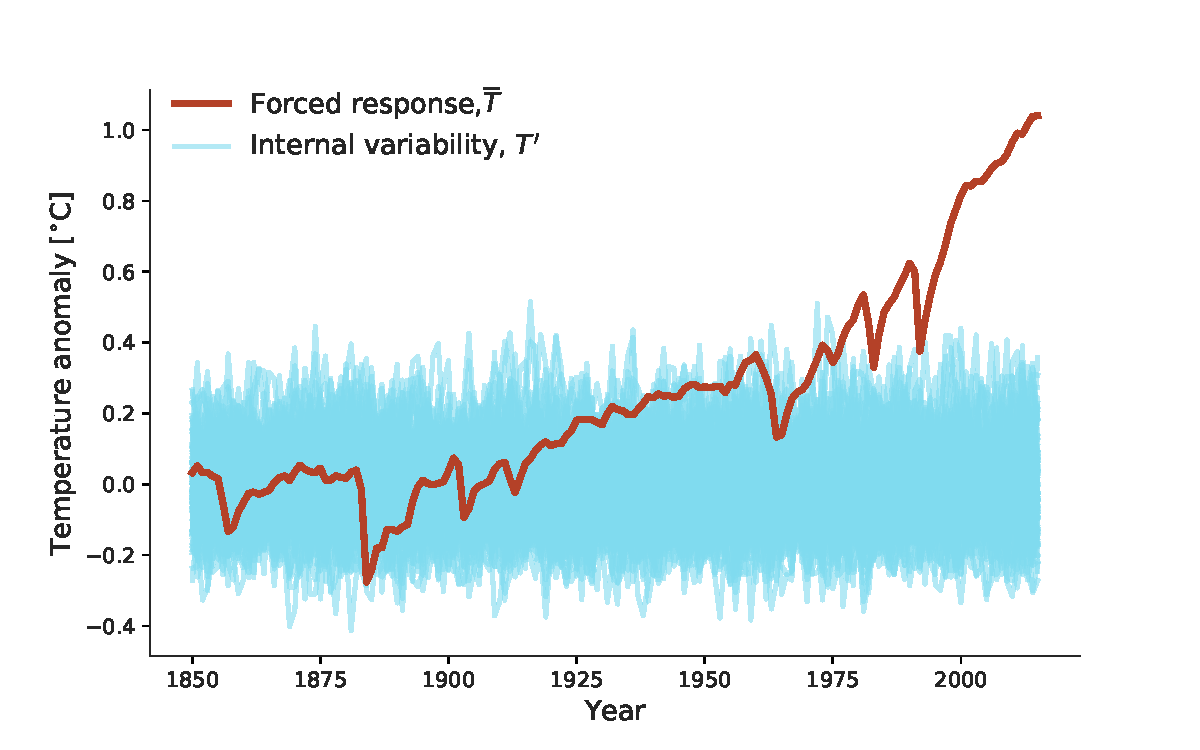
\includegraphics[width=12 cm]{../plots/Variability03.pdf}
	\end{center}
	\caption{ Caption } 
	\label{fig:variability_03}
\end{figure}

\section{Noise}
Not everyone has a large ensemble. And for purposes of efficiency or conceptual understanding, we may wish to represent variability in a simpler way than with a coupled climate model. We can represent internal variability in the simple models we have already encountered by replacing the forcing with an error term. In the mixed layer model this becomes:

\begin{equation}
C\frac{dT}{dt} = \epsilon + \lambda T,
\label{eq:mlo-var}
\end{equation}

The error term is sampled from a Gaussian distribution $\epsilon \sim N(\mu,\sigma^{2})$, and is independent of past error terms, like rolling a die. We call this type of stochastic process \textit{white noise}. 

So, how does the surface temperature respond to white noise in the forcing? Do we also expect it to have a white noise signature? Not really, since the temperature is not independent at each timestep. If we look back to Equation \ref{eq:numerical_solution} and rearrange, we clearly see the temperature has a memory of the previous timestep.
\begin{equation}
T(t+\Delta t) =  \left[1 + \frac{\Delta t \lambda }{C}  \right] T(t) + \frac{\Delta t}{C} \ \epsilon(t), 
\end{equation}
The dependence on the previous timestep is reminiscent of a process we call \textit{red noise}.

We can visualise the different colours of noise in our system by calculating their power spectral density. The power spectral density $P$ is a measure of the power at each frequency, which in our system is analogous to the strength of the variability at different time lags. With model output we can calculate $P$ for our desired variable $x(t)$ using a Fourier Transform:
$$P = \left | \mathcal{F}\{x(t)\}\right | ^{2}$$

Alternatively, and this I find more intuitive for understanding the concept of noise, we can perform a Fourier Transform on the autocorrelation function of $x$:

$$P = \mathcal{F}\{\gamma(\tau)\} ,$$

If we standardise our variable $x$, so that $x \sim (\mu=0,\sigma^{2}=1)$, we can write the autocorrelation function as

$$\gamma(\tau)\ =  \overline{x(t) \ x(t+\tau)}$$.

For white noise, this becomes a delta function, since for $\tau = 0$, the autocorrelation is equal to the variance, which is $=1$ by definition, and for all other time lags the correlation is 0.
$$\gamma_{W}(\tau)\ =  \overline{x(t) \ x(t+\tau)} = \overline{\epsilon(t) \ \epsilon(t+\tau)} = \delta(0)$$. The power spectrum then takes on a constant value for all frequencies
$$P = \mathcal{F}\{\gamma_{W}(\tau)\} = const. $$.

Our temperature variable is a bit trickier. If we assume that it is a standardised red noise process, it will take the form
$$x(t+1) = a x(t) + \sqrt{1-a^{2}} \ \epsilon(t),$$
and the autocorrelation for $\tau = 1$ is

\begin{equation}
\begin{aligned}
\gamma_{R}(1) = {} &  \overline{x(t+1)  x(t)}  = a \overline{x(t)^{2}} + \sqrt{1-a^{2}} \ \overline{\epsilon(t)x(t)}  \\
& = a \cdot 1 + \sqrt{1-a^{2}} \cdot 0 = a
\end{aligned}
\end{equation}

Successive autocorrelation coefficients go like $a^{\tau}$, and although these are discrete values, we can cheat a little and write the autocorrelation function as a continuous function. We also make the function `even' by taking the absolute value of $\tau$, since by definition $\gamma(\tau) =\gamma(-\tau)$:

\begin{equation}
\gamma_{R}(\tau) = a^{|\tau|} = e^{-R |\tau|}  \\
\end{equation}
where $R = ln(a) > 0 $. It can be shown that the Fourier transform of such a function and therefore the Power spectrum is
$$P_{R} = \mathcal{F} \left \{ e^{-R |\tau|} \right \} = \frac{2R}{R^{2} + \omega^{2}}   \\$$
where $\omega$ is the frequency.

We can now plot the power spectra for both white and red noise and appreciate their distribution.

\begin{figure}
	\begin{center}
		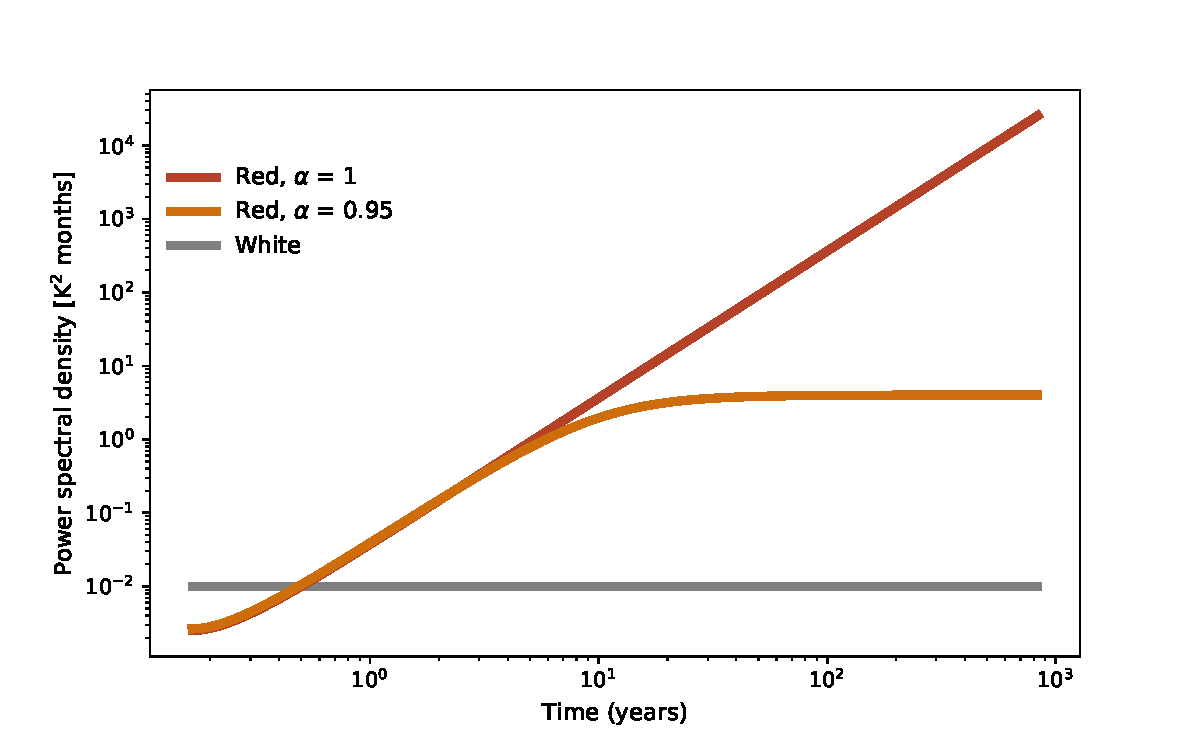
\includegraphics[width=14 cm]{../plots/Variability04.pdf}
	\end{center}
	\caption{ Caption } 
	\label{fig:variability_04}
\end{figure}




\section{Climate response to noise}
What happens in the mixed and two-layer model?
Influence of the deep ocean. Perhaps refer to Uwe and Ernst Meier-Reimers paper
May consider ECS and influence on auto-correlation.






%---------------------------------------------------------------------
\chapter{Historical warming}
\label{chapter:historical}

The recent global warming found in the instrumental record plays a central role in the debate over anthropogenic climate change. It is the best observed example of climate change we have, but unfortunately it is caused by a large number of factors that complicates interpretation.

\section{Historical forcings}
Human activity, the sun and volcanoes have had important impacts on the Earth's radiation balance in the past few centuries. In chapter \ref{chapter:forcing} we had a more detailed look at CO$_2$ forcing and the associated adjustments, but there are many other ways that human activity affects climate and CO$_2$ is probably just half of the sum off all positive impacts by human activities. Figure \ref{fig:ipcc_forcing} displays the many different components and estimates of their uncertainties. We could probably spend a lecture on each of them, just like we did it for CO$_2$, but in the interest of here I explain them only roughly and estimate the timescales involved:

\begin{figure}[b!]
\begin{center}
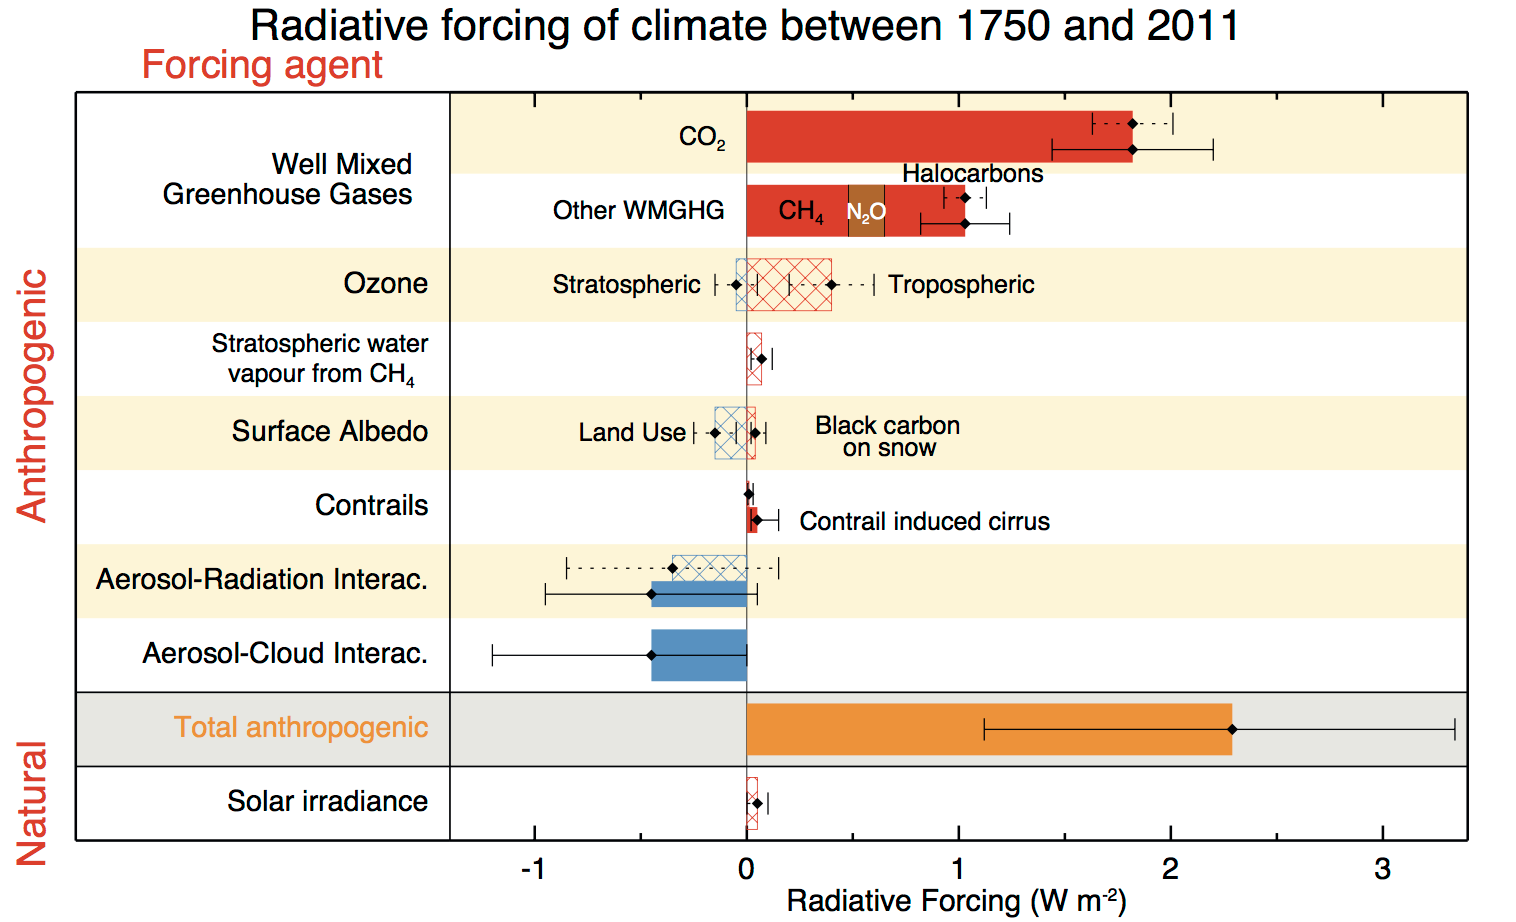
\includegraphics[width=12 cm]{../external_figures/AR5_radiative_forcing.png}
\end{center}
\caption{ Estimates of radiative forcing from the latest IPCC AR5 report. } 
\label{fig:ipcc_forcing}
\end{figure}

\begin{figure}
\begin{center}
\includegraphics[width=12 cm]{../plots/Forcing_two_layer_model_historical.pdf}
\end{center}
\caption{ Time series of annual mean globally averaged forcing estimates relative to year 1850.  Data are from the IPCC AR5 WG1 (http://www.climate-change2013.org/images/report/WG1AR5\_AIISM\_Datafiles.xlsx. } 
\label{fig:historical_forcing}
\end{figure}

\begin{itemize}
\itemsep0em
%\setlength\itemsep{0 cm}
\item�CO$_2$ is emitted from fossil fuel burning and is partly stored on a short timescale in the atmosphere, partly in vegetation and the upper ocean. It is the most important positive forcing. CO$_2$ is chemically inert, and is only slowly removed into the deep ocean and eventually sediments on timescales of centuries to multiple millennia. 
\item Other well-mixed greenhouse gases also contribute substantial positive forcing. These tend to have somewhat shorter life-times than CO$_2$, e.g. CH$_4$ stays in the atmosphere for about 10 years. 
\item Ozone change due to human activity include ozone depletion in the stratosphere and ozone increases in the troposphere as a result of pollution. The latter is more important. The lifetime of the related pollutants are roughly days to months in the troposphere and decades for those affecting ozone in the stratosphere.
\item Stratospheric water vapor can increase over natural levels due to methane oxidation (2O$_2$ + CH$_4 + \nu \rightarrow $ CO$_2$ + 2H$_2$O). The lifetime of stratospheric water is several years.
\item Land-use change from e.g. forests to agriculture has made the surface of the Earth slightly brighter, and therefore exerts a small negative forcing.
\item Contrails from high-altitude air traffic create additional cirrus clouds which have a small warming effect because they reduce the infrared radiation to space. The lifetime of these clouds are of the order of days.
\item Aerosol particles due to human activities exert a negative forcing on the Earth, both directly by reflecting sunlight back to space and through cloud adjustments. Some aerosol particles can also preferentially absorb sunlight thereby having a warming effect, in particular over bright surfaces. The clouds adjust to aerosol particles for instance because cloud droplets require an aerosol particle that can act as condensation nuclei. There are many processes involved and therefore estimates are uncertain. The typical lifetime of aerosol particles is a week.
\end{itemize}
In Figure \ref{fig:historical_forcing} I display the evolution in time of the best estimates of some of the more important components.




\vspace{0.5 cm}
\noindent
The natural forcing arises mostly from solar variability and volcanic eruptions. The sunlight input can vary if the either the Earth's orbit changes or the solar activity affects the solar irradiance. Over the period of about 150 years the orbit does not change much, this is more relevant at timescales of 10,000 years and longer; the so-called Milankovitch cycles thought to control the ice-ages. The irradiance varies also over long timescales, but it also has a distinct cycle around 11 years, clearly visible in Figure \ref{fig:historical_forcing}. This cycle plays for instance a role in the flattening of the forcing in the first decade of the 21st Century.
The strong negative spikes in volcanic forcing happens when volcanoes are explosive enough to inject material into the stratosphere. If the material does not make it up to the stratosphere it is generally precipitated out in a matter of weeks, but once in the stratosphere it can stay aloft for a year or longer and therefore begin to have an appreciable impact on the temperature. Except perhaps for Pinatubo that erupted in 1991, the forcing of individual volcanic eruptions are not very well known. 

The plot of the forcing since 1850 can be deceiving in at least two ways. First, anthropogenic forcing wasn't exactly zero in 1850. The greenhouse gas forcing was already estimated to be around +0.3 Wm$^{-2}$ relative to 1750, but it is thought that the early industry emitted enough aerosol to compensate the greenhouse gas forcing in the global mean. The second point is more subtle and relates to how we think of volcanoes. These are a natural, and for all we know, randomly occurring cooling. So a system that is not forced by human activity will see an average forcing of the longterm mean and equilibrate with it, and so the best way to think of volcanic forcing is in terms of deviations from this mean. This also means that periods without volcanoes will be warmer than usual, implying that actually the volcanic forcing is positive. It is left as a project to estimate the effect of how we handle volcanic forcing.

\begin{figure}
\begin{center}
\includegraphics[width=12 cm]{../plots/Temperature_two_layer_model_historical.pdf}
\end{center}
\caption{ Temperature evolution in the two-layer model with the historical forcing estimates displayed in Figure \ref{fig:historical_forcing}. In these runs ECS is set to 1.78 K, for reasons that shall become apparent. The observed temperature is shifted such as to have the same mean as the model over the period 1850-1879. } 
\label{fig:historical_two-layer}
\end{figure}

We can take the forcing time series and apply them to the two-layer model, equations \ref{eq:twolayer-deep}-\ref{eq:twolayer-ml}, we developed in Chapter \ref{chapter:evolution}. The result is shown in Figure \ref{fig:historical_two-layer}, where I have run the model for both the combined forcing and for the individual components shown in Figure \ref{fig:historical_forcing}. We see that the two-layer model does a decent job in matching the observed warming, whereby one should remember that the two-layer model does not exhibit natural variability such El Ni\~no, which is visible in the global mean temperature in for instance in 1997/98 and in 2015/16. 


\section{Interpreting historical warming}
It has now become popular to try to infer $ECS$ from the historical warming. 
I showed in chapter \ref{chapter:evolution} that the two-layer model can be reduced to the zero-layer model with reasonable approximation if the forcing changes gradually on decadal time-scales. I repeat the zero-layer model here:
$$T(t) = \frac{F(t)}{\gamma-\lambda}$$
and the planetary imbalance is:
$$N(t) = \gamma T(t),$$
where we remember that $\lambda$ is the feedback parameter which is negative for stable systems, and $\gamma$ is the deep ocean heat uptake coefficient which is on the order of 1 Wm$^{-2}$K$^{-1}$.
Now we are interested in estimating Earth's equilibrium climate sensitivity, $ECS=-F_{2x}/\lambda$, based on the observed warming. If we assume the zero-layer model applies we may simply compare two different times, $t_1$ and $t_2$, since $T$ and $F$ are proportional and define differences such that e.g. $\Delta T = T(t_2)-T(t_1)$ to get:
$$\Delta T = \frac{\Delta F}{\gamma-\lambda}$$
and 
$$\Delta N = \gamma \Delta T.$$
Next, we can eliminate $\gamma$ by combining the two equations, and then insert the definition of $ECS$ in order to obtain:
$$\Delta T = \frac{\Delta F}{\frac{\Delta N}{\Delta T}+\frac{F_{2x}}{ECS}}$$
and re-arrange in order to isolate $ECS$:
\begin{equation}
ECS = \frac{F_{2x}\cdot \Delta T}{\Delta F - \Delta N}.
\label{eq:zero_ecs}
\end{equation}

\noindent
Now we see that the problem of determining ECS boils down to estimating the change in temperature, forcing and planetary imbalance between two periods. The periods can in principle be chosen freely, it is not required that one period is at stationarity. It is, however, important that the assumptions made in the zero-layer model are reasonable fulfilled, for instance that the forcing is changing gradually on decadal time-scales. Looking at figure \ref{fig:historical_forcing} we see that volcanic forcing is the perfect counter-example of a gradually changing forcing. This leaves us with periods in the late 19th Century, one in the mid-20th Century and the early 21st Century. In table \ref{table:input} I provide the difference between the former and the latter. 

\begin{table}
  \caption{Input for the observations-based analysis. Changes are between the period 2005-2015 minus 1859-1882. Uncertainties are standard deviations of the assumed gaussian distributions. The lower part of the table specifies the individual contributions to the total forcing change.  }
  \vspace{0.5 cm}
  \centering
  \begin{tabular}{lrlr}
    \hline
    Quantity & Value &  & Source\\
    \hline
    Temperature change, $\Delta T$     & 0.77&$\pm$ 0.08 K                  & HadCRUT4\citep{Morice:2012dw} \\
    Total forcing change, $\Delta F$      & 2.16&$\pm$ 0.59 Wm$^{-2}$   & IPCC\citep{IPCC:2013is} \\    
    Planetary imbalance, 2005-2015, $N(t_2)$            & 0.71&$\pm$ 0.06 Wm$^{-2}$   & Johnson et al.\citep{Johnson:2016do} \\
    Planetary imbalance, 1859-1882, $N(t_1)$                     & 0.15&$\pm$ 0.075 Wm$^{-2}$ & Lewis and Curry\citep{Lewis:2014jt} \\    
    \hline
    Greenhouse gas forcing change   & 2.53&$\pm$ 0.18 Wm$^{-2}$   & IPCC\citep{IPCC:2013is} \\    
    Aerosol forcing change                  &-0.69&$\pm$ 0.55 Wm$^{-2}$   & IPCC\citep{IPCC:2013is} \\    
    Black carbon on snow change      & 0.02&$\pm$ 0.02 Wm$^{-2}$   & IPCC\citep{IPCC:2013is} \\     
    Stratospheric water vapor change& 0.06&$\pm$ 0.03 Wm$^{-2}$   & IPCC\citep{IPCC:2013is} \\        
    Land use change                          &-0.10&$\pm$ 0.06 Wm$^{-2}$   & IPCC\citep{IPCC:2013is} \\        
    Ozone change                              & 0.29&$\pm$ 0.12 Wm$^{-2}$   & IPCC\citep{IPCC:2013is} \\        
    Contrails                                        & 0.05& Wm$^{-2}$                     & IPCC\citep{IPCC:2013is} \\        
    Natural forcing change                  & -0.005 &  Wm$^{-2}$                & IPCC\citep{IPCC:2013is} \\ 
    \hline
    Forcing for doubled CO$_2$ ($F_{2\times}$)           & 3.71&$\pm$ 0.26 Wm$^{-2}$   & \\        
    \hline
  \end{tabular}
  \label{table:input}
\end{table}

Inserting values from Table \ref{table:input} in Equation \ref{eq:zero_ecs} we obtain $ECS \approx$ 1.78 K. This number is fairly low compared to suggestions that $ECS$ likely is between 1.5 and 4.5 K, a result that has puzzled scientists in the past five years. There are a number of suggestions out there for why these estimates are low-biased ranging from the temperature record not having global coverage, that feedback is non-constant between decadal and centennial timescales, natural variability, to forcings act differently and cannot simply be added.

Here we shall instead look at what the uncertainty in each term in equation  \ref{eq:zero_ecs} means for uncertainty in $ECS$ inferred by this method. It is not so straight-forward (I believe it is impossible) to use regular error-analysis that you might have learned in earlier courses because of the division by a difference. Further, not all errors are independent. For instance the change in $\Delta F$ contains a contribution from CO$_2$ that has errors that are dependent on errors in $F_{2x}$. Therefore we resort to Monte-Carlo sampling.

In Monte-Carlo sampling methods you assume probability-distribution functions for all terms in the expression you are interested in estimating (e.g. equation \ref{eq:zero_ecs}), then draw random samples from those distributions. The random samples are then used to evaluate random estimates of the expression. Here we shall use the gaussian distribution, referred to as the normal distribution. In Python you can the ask for example for 10 samples from the gaussian distribution with mean equal 0.0 and standard deviation of 1.0 as follows:
\begin{verbatim}
   > import numpy as np
   > np.random.normal(0.0, 1.0 , 10)
      1.52  -0.31  -0.28  -0.18  -0.52  0.16  0.71  1.24  0.81  -0.58 
\end{verbatim}
If you would sample enough, perhaps a few million times, and plot the probability distribution you would get something very close to a gaussian distribution.

Now we can do the same for each quantity in equation \ref{eq:zero_ecs}. We will simply assume that they are gaussian with the standard deviations listed in Table \ref{table:input}. Already by looking at the uncertainties it is clear that the numerator is fairly well constrained with errors of about 10 percent, but the denominator $(\Delta F - \Delta N)$ can cause more uncertainty in $ECS$. This is particularly the case if $\Delta F$ becomes small so that we divide by a small number and $ECS$ can become large. 
In figure \ref{fig:ECS_inferred_forcing} I plot the non-aerosol and the aerosol forcing, and their sum. We see how aerosol forcing is assumed much more uncertain than the uncertainty in all other forcing components together, and that aerosol forcing is dominating the uncertainty in total forcing. We can understand this as for independent random errors the standard deviations add in quadrature, such the standard deviation of the total forcing is the square root of the sum of squared standard deviations:
$$ \sigma_{total} = \sqrt{\sigma_{aerosol}^2 + \sigma_{non-aerosol}^2}$$

\begin{figure}
\begin{center}
\includegraphics[width=10 cm]{../plots/ECS_inferred_forcing.pdf}
\end{center}
\caption{ Monte-Carlo sampled forcing change used to estimate $ECS$ from historical warming. I plot probability distributions for aerosol, non-aerosol and total forcing change. } 
\label{fig:ECS_inferred_forcing}
\end{figure}

With the resulting distribution of $\Delta F$, and likewise randomly sampled $\Delta T$ and $\Delta N$, we can now calculate a corresponding distribution of $ECS$ following equation \ref{eq:zero_ecs} as displayed in Figure \ref{fig:ECS_inferred}. We see that the method results in a highly skewed distribution giving most weight to lower-end $ECS$ and a long tail towards higher values (actually, a few samples have $ECS > \infty$). Given the strong weight on low-end $ECS$ this type of estimates is somewhat at odds with other evidence suggesting $ECS$ is most likely around 3 K, or sometimes higher. One possible reason for this could be that the feedback parameter is different when the system is out of balance; an effect we shall investigate in the next chapter.

\begin{figure}
\begin{center}
\includegraphics[width=10 cm]{../plots/ECS_inferred.pdf}
\end{center}
\caption{ Monte-Carlo sampled probability distribution of $ECS$ as calculated using equation \ref{eq:zero_ecs} using values from table \ref{table:input}. The median value and the 5-95 percent interval of the distribution is printed. Here I have additionally sampled $F_{2x}$ in such a way that it correlates with greenhouse gas forcing, though this has  little impact on the results and can be ignored. } 
\label{fig:ECS_inferred}
\end{figure}




%---------------------------------------------------------------------
\chapter{State-dependent feedback}
In the previous chapters we assumed that perturbations were small enough that feedbacks could be considered approximately constant. However, there are good reasons to think that for even modestly warmer or colder climates that feedback mechanisms could change in strength. 
It turns out that all the feedbacks, surface albedo, temperature, water vapor and clouds may depend on the climate state, and understanding and quantifying the underlying processes -- and what it means for the interpretation of Earth's past and possible futures -- are subject to ongoing scientific debate. %Thus I will only discuss them qualitatively here. 



\section{Snow-ball Earth instability}
An obvious example of a state-dependent feedback is the positive surface albedo feedback from melting snow and sea-ice which must cease in very warm climates when there is no more snow or ice left to melt. Or, likewise, if it gets so cold that the entire Earth's surface is covered with snow and ice, then surface albedo feedback also ceases. In between these extremes there must be a maximum, a fact that can lead to the classical snow-ball Earth instability. There is some geological evidence that such nearly frozen over states may have occurred in the early history of Earth.

To approach the problem let us consider the gray body case. We remember that the energy imbalance is the difference between the absorbed sunlight and the emitted infrared radiation to space, where we model the latter via an emissivity, $\epsilon$:
\begin{equation}
N = \frac{S_o}{4}(1-\alpha) - \epsilon \sigma T_s^4
\label{eq:gray_body_2}
\end{equation}
where for present-day Earth-like conditions $T_s\approx 288$ K, $\alpha \approx 0.29$ and $\epsilon \approx 0.61$, and we have shown in an exercise that the equilibrium surface temperature at $N=0$ is:
$$T_s = \sqrt[4]{\frac{S_o(1-\alpha)}{4\epsilon\sigma}}.$$
Now, let us imagine that the planetary albedo ($\alpha$) no longer a constant but instead it is a simple function of global mean surface temperature such that:
%\[
\begin{equation}
\alpha(T_s) = 
\begin{dcases*}
   \alpha_i                    & $T_s \le T_i$  \\
   \alpha_o+(\alpha_i-\alpha_o)\frac{(T_s-T_o)^2}{(T_o-T_i)^2}       & $T_i < T_s \le T_o$ \\
   \alpha_o                    & $T_o < T_s$ 
\end{dcases*}
\label{eq:snowball}
\end{equation}
%\]
where I have chosen $T_i=250$ K, $T_o=288$ K, $\alpha_i=0.70$ and $\alpha_o=0.29$. The quadratic behavior of the planetary albedo is intended to emulate the effect that the further equatorward the ice extends the larger the incremental area increase per degree cooling becomes, and thereby the feedback becomes stronger. One can use a linear relationship too for the considerations made here, whereby one would need to lower the $T_o$ parameter to avoid an almost immediate freeze-up. The choice of $\alpha_i$, corresponding roughly to a fully snow-covered state, is rather extreme as a snow-ball Earth will have mostly aged snow or regional bare ice surfaces which are darker, and supposedly there might also have been a rim of open ocean around the equator. Instability could also occur for a weaker state-dependence if $\epsilon$ is allowed to vary, for instance due to water vapor feedback.

\begin{figure}
\begin{center}
\includegraphics[width=12 cm]{../plots/Snowball_Earth_budget.pdf}
\end{center}
\caption{ Plot of the right-hand-side terms of equation (\ref{eq:gray_body_2}) combined with equation (\ref{eq:snowball}): blue is absorbed sunlight, red is emitted infrared radiation. Dashed curves show bifurcations for blue reduced solar input at $S=0.87\cdot S_o$ and for red reduced emissivity of $\epsilon=0.46$. } 
\label{fig:snowball}
\end{figure}

It is possible to solve algebraically for fix-points, but for simplicity I plotted the two terms on the right-hand-side of equation (\ref{eq:gray_body_2}) in figure \ref{fig:snowball} as thick solid blue and red lines to see that three solutions of $N=0$ corresponding to $S_o/4\cdot(1-\alpha)=\epsilon \sigma T_s^4$ are possible with our choice of parameters at $T_s \approx 233$ K,  $T_s \approx 258$ K and  $T_s \approx 289$ K. We recognize the latter as the present-day solution and the first solution is the snow-ball state. 
The intermediate fix-point at $T_s \approx 258$ K turns out to be unstable (see Chapter \ref{chapter:response}). This is because at temperatures just above the fix-point the imbalance is positive ($S_o/4\cdot(1-\alpha) > \epsilon \sigma T_s^4$) such that the system would warm up and therefore move away from the fix-point. Likewise, for temperatures just below we have a negative imbalance ($S_o/4\cdot(1-\alpha) < \epsilon \sigma T_s^4$) and the system would cool off, again moving away from the fix-point. We remember from Chapter \ref{chapter:response} that a fix-point is unstable if the feedback parameter at that point is positive: 
\[
\lambda = \frac{dN}{dT_s} = -\frac{S_o}{4}\frac{d\alpha}{dT_s}-4\epsilon \sigma T_s^3 > 0
\]
that is, in this case the slope of the absorbed shortwave (blue) is steeper than the slope of the emitted longwave radiation (red). The opposite is the case for the snow-ball and present-day states, such that these are stable stationary states: the solution will return to the fix-points if we add or subtract small fluctuations. The solutions are not unconditionally stable, though. If you perturb it really hard ($\approx$ 30 K) the system can transition to the other stable state. 

\begin{figure}
\begin{center}
\includegraphics[width=11 cm]{../Plots/Snowball_Earth_pseudo_potential.pdf}
\end{center}
\caption{ Pseudo potential curve for the snow-ball Earth instability case. The system has three equilibria $V$ is local minimum or maximum, two of which are stable and one is unstable.  } 
\label{fig:snowball_pseudo_potential}
\end{figure}

It can be illustrative to calculate the pseudo potential for cases such as the snow-ball Earth case that have multiple equilibria. We can define the pseudo potential, $V$, as:
\[
-\frac{dV}{dT_s} = N
\]
such that at fix-points where $N=0$ we have that $V$ has zero slope. This means that $V$ is either a local minimum or maximum, or possibly a saddle point. We further remember that the feedback parameter is $\lambda = dN/dT_s$ such that the stability of a fix-point can be inferred from the second derivative of the pseudo potential: if $V$ is a local minimum then the fix-point is stable, if it is a local maximum the fix-point is unstable. A saddle point has marginal stability. It is easy to calculate $V=-\int N dT_s$ and I show the result in Figure \ref{fig:snowball_pseudo_potential}. It is tempting to imagine the curve as a hilly landscape where the system will try to gravitate towards either of the two minima, depending on where it starts from. 

Changing the parameters of the model can lead to bifurcations whereby the number of fix-points change. As the most simple example, if there is no greenhouse effect ($\epsilon=1.0$, black curve) then there is only one solution at:
$$T_s= \sqrt[4]{\frac{S_o(1-\alpha_i)}{4\sigma}} \approx 206 \textrm{ K},$$
where I assume that the solution is safely below $T_i$. This is substantially below the black-body solution with present-day planetary albedo ($T_e\approx 255$ K) because there is simply less sunlight being absorbed in the snow-ball state.

Perhaps more interesting is what happens if one lowers the solar constant. Then the warm-state fix-point cools off and the intermediate fix-points warms such that they eventually collide. This situation is depicted by the blue dashed line in Figure \ref{fig:snowball}. In this case the fix-point becomes marginally stable (Figure \ref{fig:feedback_stability_cases}), which means that it is stable to positive perturbations but unstable to negative perturbations, as in both case $N$ becomes negative a bit away from the fix-point. This means that, eventually, the system will transition towards the snow-ball state. 

Once the system is in the snow-ball state then how could it transition back to the warm state? One could imagine increasing the solar constant, but given what we know about our sun's past history it seems unlikely to have happened. The other option is to increase the greenhouse effect, i.e. to lower $\epsilon$, but by how much? We can use the fact that the transition will happen when the snow-ball fix-point reaches $T_o$ and thereby estimate the critical emissivity:
$$
\epsilon_c = \frac{S_o}{4}\frac{1-\alpha_i}{\sigma T_i^4} \approx 0.46.
$$
The case is depicted as the red dashed curve in Figure \ref{fig:snowball}. The fix-point is again marginally stable and so is stable to negative perturbations, but unstable to positive perturbations, and thus will eventually end up in the warm state. It will actually take quite a bit of greenhouse gases to bring the system out of a snow-ball state, in particular because the greenhouse effect from water vapor is small at such cold temperatures.

The behavior can be illustrated with a modified version of the two-layer model, whereby I use absolute temperature and equation \ref{eq:gray_body_2} for the energy balance (Figure \ref{fig:snowball_twolayer}); it should be noted that the two-layer model would need some modification to do a reasonable job in handling an ice-covered ocean, even if this is less relevant here. First we note that at standard settings the initial conditions determine at which solution the system ends: if it starts in the warm state it stays there (black), and if it starts in the snow-ball state it stays there (red). Then, starting from the warm state I scale the solar constant down relative to its present-day value ($S_o$). When I lower $S$ to $0.88\cdot S_o$ the system cools but stays in the warm state, but at $0.87$ suddenly a rapid transition occurs to the snow-ball state. The last example show how a lowering of $\epsilon$ can allow the system to escape the snow-ball state (orange).

%The case with 0.88 is however not stable to perturbations which can be seen from an additional run where I add random noise to the radiation balance. In this case the system cools a bit faster and eventually transitions to the snow-ball state after about 1,000 years. This goes to show that when considering also natural variability the system need not to reach the bifurcation before a transition can occur.

\begin{figure}
\begin{center}
\includegraphics[width=13 cm]{../plots/Two_layer_snowball.pdf}
\end{center}
\caption{ Qualitative behavior around the snow-ball instability depending on initial  and boundary conditions. %All but the orange case starts at present-day temperatures. The orange case illustrates how the system can exit the snow-ball state if there is a low enough emissivity.  
} 
\label{fig:snowball_twolayer}
\end{figure}


\section{State-dependent feedbacks in a warmer world}
Next we will consider cases that are warmer than present. Evidence from the Eocene period about 50 million years ago (Figure \ref{fig:Paleo_temperature_timeseries}), when the Earth was warmer than it is today, suggests that $ECS$ was also higher than today -- around twice as large. It is currently not known why that might have been. Some climate models are capable of producing a rise in $ECS$ in warmer climates, but studies find different magnitudes as well as causes for the rise depending on which model and methods are used. And some models do not even exhibit an increase of their $ECS$ in a warmer climate. 

One model that does exhibit a substantial rise in $ECS$ in a warmer climate is the MPI-ESM1.2 (Figure \ref{fig:mpiesm12_wide_range}). We can see how the model exhibits a relationship between $T_s$ and $N$ that is far from linear when exposed to strong forcing, here an abrupt increase of CO$_2$ to sixteen times the pre-industrial level (16xCO$_2$). Remember that the forcing from CO$_2$ is roughly logarithmic in the concentration so that each doubling results in about the same amount of forcing. 
It will take a few thousand years to equilibrate a coupled model with a forcing, and so the displayed runs have not yet reached a stationary state. But we can get a good idea of where the runs are headed by fitting a line to the output and then extrapolate to zero. Because of the bending I chose to use the years 100 to 1000 of each run for the estimate; the results are shown in the lower part of Figure \ref{fig:mpiesm12_wide_range}. We can now estimate $ECS$ for each of the doublings as the difference between the equilibria:
\begin{center}
\begin{tabular}{l|r} 
 & $ECS$  \\
\hline
1xCO$_2$ to 2xCO$_2$     & 2.77 K \\
2xCO$_2$ to 4xCO$_2$     & 3.61 K \\
4xCO$_2$ to 8xCO$_2$     & 4.92 K \\
8xCO$_2$ to 16xCO$_2$     & 9.80 K 
\end{tabular}
\end{center}
where we see that $ECS$ roughly triples from the first to the fourth doubling of CO$_2$. The difference is mainly due to a change in slope, which we remember is the feedback parameter. On the contrary, the forcing from each doubling is not changing in a way that explains the rise in $ECS$. 

\begin{figure}
\begin{center}
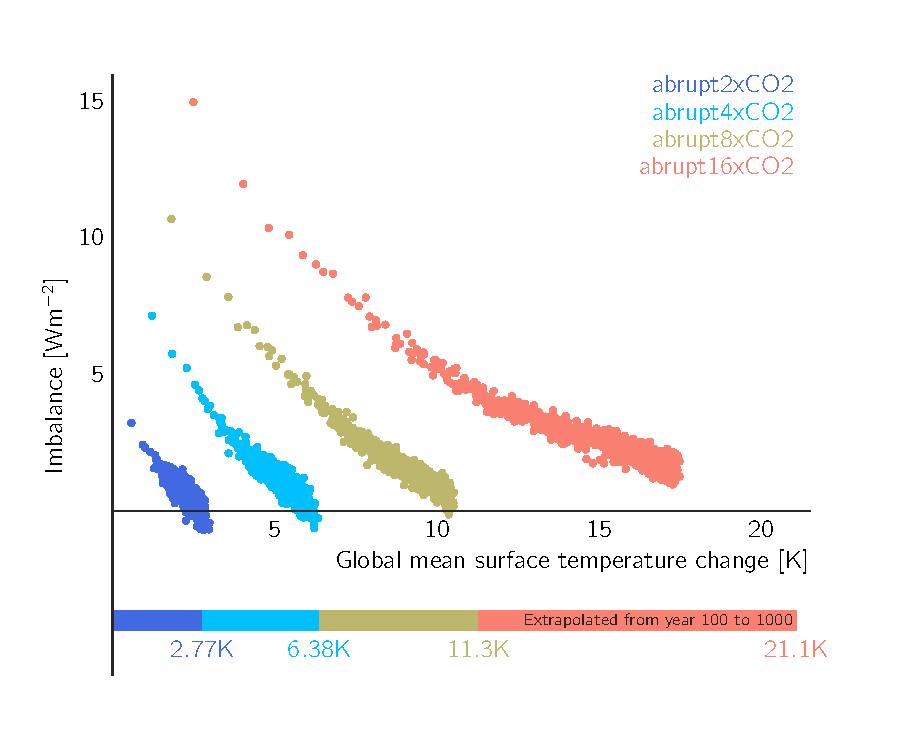
\includegraphics[width=12 cm]{../external_figures/MPI-ESM12_gregory_plot.pdf}
\end{center}
\caption{ Gregory plot of four simulations with the MPI-ESM1.2 model. Each simulation is 1000 years. The equilibrium temperature is estimated by linearly extrapolating the years 100 to 1000 of the simulations. } 
\label{fig:mpiesm12_wide_range}
\end{figure}

\subsection{Possible mechanisms}
Next, we will explore why $ECS$ increases in MPI-ESM1.2. Here the reader is cautioned, though, that the mechanisms are different between models, even model versions as I found quite different results for the predecessor of this model (MPI-ESM). 
We now can analyse these runs as we did in Chapter \ref{chapter:forcing} by splitting up the radiation balance into contributions from temperature, water vapor, clouds and surface albedo: $N=N_T+N_W+N_C+N_A$. The evolution of the four terms are shown in Figure \ref{fig:state_dependent_feedback_mpiesm12}. At first sight, not much changes across the displayed range. But one has to remember that it is the sum of four components that make up the total imbalance. I calculated the slope of each term on years 100 to 300 for the two runs:
\begin{center}
  \begin{tabular}{l|rr} 
Feedback parameter (Wm$^{-2}$K$^{-1}$) & 2xCO$_2$ & 16xCO$_2$  \\
\hline
Temperature     & -4.21  & -4.19 \\
Water vapor      & 2.20 & 2.71 \\
Clouds              & 0.30 & 1.01 \\
Surface albedo & 0.23 & -0.01
  \end{tabular}
\end{center}
From this we see that the positive change in the total feedback parameter is not due to changes in the temperature and surface albedo feedback parameters in this model. In fact, surface albedo feedback diminishes to near-zero in the warm climate thereby counteracting the rise in $ECS$. Instead it is water vapor and cloud feedbacks that cause the rise in sensitivity in warmer climates. 

\begin{figure}
\begin{center}
\includegraphics[width=10 cm]{../plots/MPI-ESM12_abrupt_forcing.pdf}
\end{center}
\caption{ Partial radiative perturbation analysis showing temperature (green), water vapor (brown), cloud (blue) and surface albedo (orange) feedback from two experiments, 2xCO$_2$ (circles) and 16xCO$_2$ (crosses) also shown in Figure \ref{fig:mpiesm12_wide_range}. Here the first 300 years are shown.   } 
\label{fig:state_dependent_feedback_mpiesm12}
\end{figure}

Clouds are the main contributors to the rise in $ECS$ in MPI-ESM1.2. However, clouds and their feedbacks on climate change can depend on so many factors that I would rather not even begin to discuss this. Clouds are also, not surprisingly, the main cause of inter model spread in state-dependence. Instead, here I will take a closer look at the other three feedback mechanisms which may act as a basis for understanding before adding the complexity of clouds.

\subsubsection{Water vapor feedback}
There is broad agreement among models of various types that water vapor feedback will get stronger in a warmer climate. 
To be honest, I am actually not quite sure why that is. 
I think, though, that it has to do with the water vapor absorption bands, unlike those of CO$_2$, being far from saturated such that the atmosphere can be considered optically thin with respect to water vapor. This also means that some of the radiation emitted by the surface escapes directly to space. As temperature rise the water vapor content increases roughly exponentially. The induced greenhouse effect, though, increases faster than logarithmically, and so the end result is a strengthening water vapor feedback. 
Beware, though, that I am here at the limit of my understanding. 


%\subsubsection{Cloud feedback}


\subsubsection{Surface albedo feedback}
Whereas the surface albedo feedback from melting snow and ice may have played an important role in climates colder than present, as we saw in the example of the snow-ball Earth instability, it will not play a significant role in a warmer climate where it may be close to zero. On average, for instance, climate models predict that Arctic spring sea ice is practically gone by about 4-7 K above pre-industrial temperatures; summer sea ice a bit earlier. 
Other factors may influence the surface albedo, though, foremost vegetation or the lack thereof. For instance a forest absorbs more sunlight than grass-lands, and deserts are actually quite reflective. Thus, shifts in the extent of the different vegetation types can induce surface albedo feedbacks too.
The Earth's currently remaining ice sheets, Greenland and Antarctica, would also eventually cause a surface albedo feedback as they adjust to a warmer climate. This process takes, as argued earlier, thousands of years because the ice sheets are very thick. Such a process is not included in the simulations with MPI-ESM1.2.

\begin{figure}
\begin{center}
\includegraphics[width=12 cm]{../plots/Planck_state_dependence.pdf}
\end{center}
\caption{ Temperature feedback parameters from ECHAM6 (red) from the study of Meraner et al. (2013) and two theoretical expressions. } 
\label{fig:planck_state_dependence}
\end{figure}
\subsubsection{Temperature feedback}
Perhaps the most surprising result in the feedback analysis of MPI-ESM1.2 is that temperature feedback didn't change appreciably. 
It is in fact easy to think that the Planck feedback is highly state-dependent as it contains the absolute surface temperature to the third power, equation (\ref{eq:lambda_planck}). The dependence on region is dramatic: the Planck feedback at tropical temperatures (30$^\circ$C) is almost twice as strong as that at high latitude winter temperatures (-30$^\circ$C). This is of course a large temperature range when thinking about global climate change, but even for more modest temperature changes the dependence is possibly of relevant magnitude because the Planck feedback is by far the largest feedback. However, things are not as simple as they might seem.
To get started we are reminded that the Planck feedback of the gray body is:
\begin{equation}
\lambda_p= -4 \epsilon \sigma T_s^3
\label{eq:planck_feedback_3}
\end{equation}
from which we see that $\lambda_p$ not only depends on $T_s$, but also on the planetary emissivity $\epsilon$. The equilibrium temperature of this system is:
\begin{equation}
T_s = \sqrt[4]{\frac{S_o(1-\alpha)}{4\epsilon\sigma}}
\end{equation}
from which we see that $T_s$ depends on $S_o$, $\alpha$ and $\epsilon$. If we now consider the case where we are increasing atmospheric CO$_2$ we can model this with small reductions of emissivity $\delta \epsilon$ corresponding to increasing the greenhouse effect:
\begin{equation}
F = - \delta \epsilon \cdot \sigma T_s^4
\end{equation}
from which we see that a one percent reduction in $\epsilon$ gives $F\approx 3.9$ Wm$^{-2}$, roughly equal to that of a doubling of CO$_2$. If we ignore any changes in $S_o$ and $\alpha$ we see that:
$$T_s \propto \epsilon^{-\frac{1}{4}}$$
Inserting this into \ref{eq:planck_feedback_3} we get that in this limiting case:
$$\lambda_p \propto \epsilon^{\frac{1}{4}}$$
which means that as the system warms due to a decreasing emissivity the Planck feedback must also weaken slowly. The case is shown in blue in Figure \ref{fig:planck_state_dependence} for a range of emissivities from 0.7 to 0.3. As a contrasting case I plotted the Planck feedback for the case that temperature increases due to an increasing solar forcing $S_o$ such that $\lambda_p \propto T_s^3$ as black. For comparison the estimates of temperature feedback, which includes Planck and lapse-rate feedbacks, from the ECHAM6 model in Meraner et al. (2013) is shown in red. The latter supports nearly constant $\lambda_T$ as also found with MPI-ESM1.2.

% It should be possible to express the state-dependence in temperature rather than emissivity which would make the result clearer. Isolate epsilon in equation 7.4 and substitute into 7.3.

\begin{figure}
\begin{center}
\includegraphics[width=11 cm]{../plots/Two_layer_like_MPI-ESM12.pdf}
\end{center}
\caption{ Simulations with the two-layer model with applied 2, 4, 8 and 16xCO$_2$ forcing, whereby the feedback parameter is assumed a linear function of temperature. Here $F_{2x}=4.5$ Wm$^{-2}$ and the base $ECS=2.6$ K, such that $\lambda_o=-1.73$ Wm$^{-2}$K$^{-1}$ and I assume a quadratic term coefficient $b=0.045$ Wm$^{-2}$K$^{-2}$. } 
\label{fig:quadratic_imbalance}
\end{figure}

\section{A quadratic representation of imbalance}
It was suggested by Bloch-Johnson et al. (2015) to represent the behavior of models, such as MPI-ESM, imbalance as a quadratic function of temperature, rather than a linear function:
\begin{equation}
N=F+\lambda_o T_s+ bT_s^2
\label{eq:quadratic}
\end{equation}
where $b$ is a coefficient, typically in the range -0.05 to 0.05. This is really nothing but a more accurate truncation of a Taylor expansion of the actual imbalance of the complex climate model. To see how well this expression works, I iteratively fitted the two-layer model (Figure \ref{fig:quadratic_imbalance}) to match roughly the behavior of MPI-ESM1.2 (Figure \ref{fig:state_dependent_feedback_mpiesm12}). The fit works reasonably well.
The system equation \ref{eq:quadratic} has one or two stationary solutions ($N=0$) given by:
$$T_s=\frac{-\lambda_o\pm \sqrt{\lambda_o^2-4bF}}{2b}$$
which has real roots for cases with positive forcing ($F>0$) only if :
$$F \le F_b=\frac{\lambda_o^2}{4b}$$
For stronger forcing ($F>F_b$) the vertex of the parabola is above zero at all temperatures, and the system finds no place to rest, warming indefinitely. When fix-points are possible, however, we can estimate their stability by calculating the feedback parameter:
$$\lambda(T_s)=\frac{dN}{dT_s} = \lambda_o+2bT_s$$
From this we can already see that the feedback parameter changes sign, and the system undergoes a bifurcation at:
\begin{equation}
T_b=\frac{-\lambda_o}{2b}
\label{eq:quadratic_runaway}
\end{equation}
such that fix-points below $T_b$ are stable and fix-points above $T_b$ are unstable. This leads to a so-called run-away feedback situation where the system warms and the imbalance increases more and more leading to further warming. This actually happens to our fit to MPI-ESM1.2 (Figure \ref{fig:quadratic_imbalance}) for a forcing corresponding to 16xCO$_2$ as shown by the dashed extension. Also the full MPI-ESM model can exhibit a run-away, even if it is difficult to make the code work at high temperatures. Popp et al. (2016) made several modifications to the model and found that the modified model has an unstable regime and if forced hard it will settle in a very warm moist greenhouse (Figure \ref{fig:popp}). In principle this situation could be modelled by adding a cubic term to equation \ref{eq:quadratic}:
$$N=F+\lambda_o T_s+ bT_s^2+cT_s^3$$
which could then have a stable fix-point at high temperatures for certain combinations of $\lambda_o$, $b$ and $c$. The overall behavior of this system is reminiscent of the snow-ball Earth instability which also had two stable fix-points with an unstable fix-point in between them.

%\section{Runaway feedback}

\begin{figure}
\begin{center}
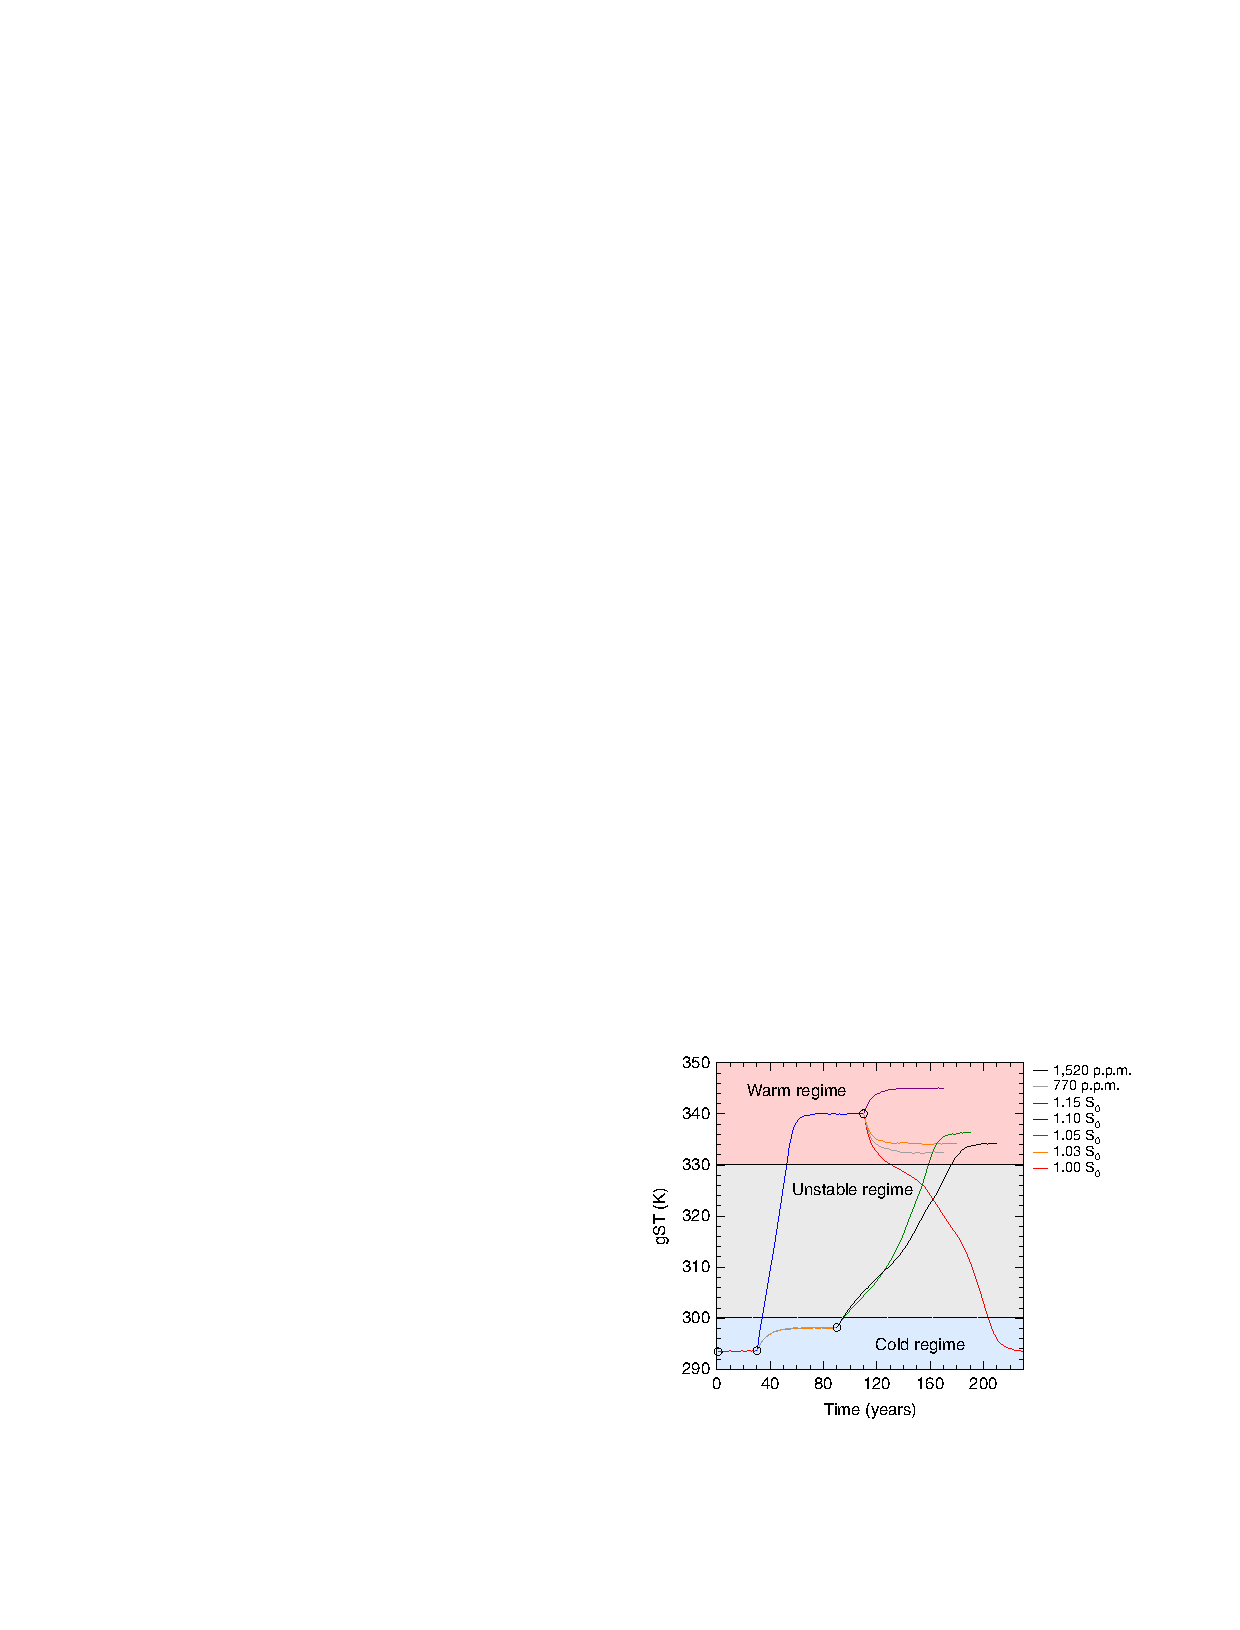
\includegraphics[width=11 cm]{../external_figures/Popp_etal_2016_instability.pdf}
\end{center}
\caption{ The transition to a moist greenhouse in model simulations by Popp et al. (2016). The model is a modified version of ECHAM6.  } 
\label{fig:popp}
\end{figure}



\newpage
\vspace{1 cm}
{\setlength{\parindent}{0cm}
%\hrule

\begin{exercise}
Calculate the feedback parameter using equations \ref{eq:gray_body_2} and \ref{eq:snowball} under present-day and last-glacial maximum conditions around 21,000 years ago (Figure \ref{fig:Paleo_temperature_timeseries}); helpful information can be found around equation \ref{eq:lambda_general}. You may here assume $\epsilon$ is constant. If you were to double CO$_2$ at these two states approximately how much would they warm, respectively? %First use the standard parameters as in the text, second try lowering $\alpha_i$ to 0.50 to account for the effects of aged snow, bare ice and some open ocean near the equator.
\end{exercise}

\begin{exercise}
A climate system has a basic state imbalance that can be approximated as $N=-1.0\cdot T_s + 0.05\cdot T_s^2$. Determine the bifurcation point temperature $T_b$ in the system and infer the stability of stationary states on either side of the bifurcation point. What will happen to the system if $T_s>T_b$?
Calculate the minimum forcing needed to cause the system to bifurcate. 
\end{exercise}

\begin{exercise}
Set up the two-layer model to run the case in the exercise above. This can be achieved by setting \verb|ECS=f2x| and \verb|b=0.05| in the function call. The former results in $\lambda_o=-1.0$ Wm$^{-2}$K$^{-1}$. Further, make sure to run the model out far enough to ensure that it can equilibrate, if possible. Since an instability may occur, you may want to limit the axis in your plot, e.g. by setting \verb|plt.xlim((0,15))| and likewise for the y-axis choosing a reasonable upper limit. 
Apply different forcing strengths and estimate iteratively at which forcing the bifurcation occurs. 
%Compare the result with the forcing needed to reach $T_b$ if $\lambda=\lambda_0$ which you can calculate analytically. %{\em Hint: it is }
\end{exercise}
}


%---------------------------------------------------------------------
\chapter{Time-dependent feedback}
The idea that climate feedbacks are time-dependent can be mind-boggling. In a deterministic dynamical system the only thing that determines the evolution moving forward in time is the current state combined with the boundary conditions. 
So when we refer to time-dependent feedbacks then formally these are also state-dependent feebdacks. 
The way I think about it is that a feedback change following the application of a forcing is defined as time-dependent if the behavior does not depend on which stationary state the system starts from or, equivalently, how strongly it is forced. This is in contrast with the examples from the previous chapter where the radiation balance depends explicitly on the temperature of the system. 
To obtain such behavior the system needs to have at least two state-variables; something which is not hard to find in the complex climate systems we often deal with. In this chapter I will go over two simple models that have exactly two state-variables such that they can exhibit time-dependency of their feedback. 
\\

A bit the background for this topic is the type of non-linearity or "bending" in a plot of imbalance versus temperature such as Figure \ref{fig:gregory_hansen} or Figure \ref{fig:mpiesm12_wide_range}, which we tried to explain in the previous chapter using state-dependent feedback. From the reasoning above it is clear that a purely time-dependent feedback cannot explain the rise in $ECS$ under strong forcing we found in MPI-ESM1.2 in the previous chapter. But there is a component to the bending that occurs in the first few decades after an abrupt forcing has been applied which does actually exhibit signs of a time-dependent behavior; something that occurs regardless how strongly the model is forced. And, there are even some climate models, such as the Hadley Centre climate model, which do not exhibit a rise in $ECS$ with warming, but still has stronger bending than MPI-ESM1.2. 
\\

The reason scientists are currently very interested in the phenomenon is that a time-dependent feedback may impact the transient response to forcing. As we shall see the time-dependent feedback can lead to a temporary suppression of warming as the system equilibrates. The effect can have important consequences for the interpretation of historical warming we made in Chapter \ref{chapter:historical}, where we assumed that the system was linear. The current challenge, I think, is to figure out {\em how} time-dependent feedback may be on planet Earth.

\begin{figure}
\begin{center}
\includegraphics[width=12 cm]{../illustrations/Time-dependent_models.pdf}
\end{center}
\caption{ Illustrations of two models which can exhibit time-dependent feedback. They each have two state-variables.  } 
\label{fig:time-models}
\end{figure}

\section{Regional feedback -- the two-zone model}
The simplest idea, as far as I know, of how feedback can be time-dependent is that different regions may equilibrate along different timescales in response to a forcing, and if they also have different feedbacks then this can lead to a time-varying globally averaged feedback. 
We might think of, say, two regions: a low-latitude region having strong negative feedback and a high-latitude region with some positive feedback mechanism, for simplicity we can think of positive snow and ice surface albedo feedback acting only at high latitudes. The low-latitudes are characterized for the most part by a relatively shallow mixed-layer, whereas at high latitudes the mixed-layer is on average deeper. 
We can model this situation with a two-zone approach as depicted in Figure \ref{fig:time-models}a. 
If there is no coupling between the regions and we assume the forcing, $F$, is the same in both regions, then we can simply model them as two mixed-layer models:
\begin{eqnarray}
C_1\frac{dT_1}{dt} &=& F + \lambda_1 T_1 \label{eq:twozone_simple} \\
C_2\frac{dT_2}{dt} &=& F + \lambda_2 T_2 \nonumber \\
N &=& w_1\cdot C_1\frac{dT_1}{dt}+w_2\cdot C_2\frac{dT_2}{dt}  \nonumber
\end{eqnarray}
where $C_1$ and $C_2$ are the heat capacities of the low- and high latitude zones, and $\lambda_1$ and $\lambda_2$ are the regional feedback parameters. Note that these equations are uncoupled, that is, the regions do not interact and we can solve the two equations separately. To get the global mean properties we need to weigh the two regions according to their extent ($w_1, w_2$); for our purposes we will assume they each cover half the Earth. This would be the case if region 1 would cover 30$^\circ$S to 30$^\circ$N latitude and region 2 the mid- and high latitudes in both hemispheres.
Because the two regions are de-coupled it is straightforward to solve the equations as the weighted sum of two mixed-layer solutions, equation \ref{eq:mlo_solution}. For instance, if we apply an abrupt forcing we get:
\begin{equation}
T(t) = -F\cdot �\left( w_1\cdot\frac{1-e^{\frac{\lambda_1}{C_1}t}}{\lambda_1} + w_2\cdot \frac{1-e^{\frac{\lambda_2}{C_2}t}}{\lambda_2} \right)
\label{eq:twozone-solution}
\end{equation}
and we can further calculate the equilibrium of the system as:
$$T(\infty) = w_1\cdot\frac{-F}{\lambda_1} +  w_2\cdot\frac{-F}{\lambda_2} $$
which is again simply the weighted equilibrium response of each region.

In equation \ref{eq:twozone-solution} we recognize the two decaying exponentials for each region with e-folding times of $\tau_1=-C_1/\lambda_1$ and $\tau_2=-C_2/\lambda_2$. Thus, if $\lambda_1$ is more negative than $\lambda_2$, then the response timescale of the high latitudes (region 2) is longer than that of the low latitudes (region 1) even in the special case where $C_1=C_2$. You might remember Figure \ref{fig:mlo_plot} where we saw that the more sensitive the mixed-layer model is the longer it takes to equilibrate. This is interesting in that it only takes spatially inhomogeneous feedbacks to cause a time-dependence of the global feedback. The different equilibration time-scale between low- and high latitudes is further amplified if $C_2 > C_1$. 

The time-dependent nature of the feedback in the two-zone model can be seen in Figure \ref{fig:two-zone-model} where I forced with 2, 4, 8 and 16 times pre-industrial CO$_2$.  The result can be compared with simulations from the MPI-ESM1.2 model (Figure \ref{fig:state_dependent_feedback_mpiesm12}) and with the quadratic model (Figure \ref{fig:quadratic_imbalance}). We see that the evolution of the model scales linearly with the forcing so that the shape of each curve is the same. If I would normalize the plot by dividing by the forcing on both axes, i.e. plot $N/F$ versus $T/F$, then the four curves would land on top of each other. If you would try to do the same normalization of runs done with the quadratic model then the curves would not be self-similar, because in the quadratic model feedback is dependent on the absolute temperature. 

\begin{figure}
\begin{center}
\includegraphics[width=12 cm]{../Plots/Two_zone_model.pdf}
\end{center}
\caption{ Solutions of the two-zone model, equations \ref{eq:twozone_simple}, with different forcing strengths. The figure is comparable to Figures \ref{fig:state_dependent_feedback_mpiesm12} and \ref{fig:quadratic_imbalance}. Here I have chosen $\lambda_1 = -3.0$ Wm$^{-2}$K$^{-1}$, $\lambda_2 = -1.0$ Wm$^{-2}$K$^{-1}$, $C_1$ corresponds to 75 m water and $C_2$ to twice that, and $F_{2x}$ is 4.5 Wm$^{-2}$ as in MPI-ESM1.2. } 
\label{fig:two-zone-model}
\end{figure}

We can also compare the result in more detail with the MPI-ESM1.2 model (Figure \ref{fig:time-dependent_abrupt4xCO2}). Here I have exaggerated the parameter choice for the two-zone model a bit, but we see that the two-zone model qualitatively replicates the type of bending that the coupled climate model has. We also see that the quadratic model, which we developed in the previous chapter, exhibits some bending but it is not as strong as in MPI-ESM1.2. One could make the quadratic model match MPI-ESM1.2 better by increasing $b$, but then the model would quickly enter a run-away because the bifurcation temperature would decrease (equation \ref{eq:quadratic_runaway}). Thus, the quadratic model may explain the increase in $ECS$, but not fully the non-linear transient behavior of MPI-ESM1.2. 

\begin{figure}
\begin{center}
\includegraphics[width=10 cm]{../Plots/Time-dependent_models_abrupt4xCO2.pdf}
\end{center}
\caption{ Solutions of the different models developed in this course forced with the equivalent of an abruptly applied quadrupled carbon dioxide (4xCO$_2$). The dashed line shows the two-zone model with a coupling coefficient of 3.9 Wm$^{-2}$K$^{-1}$. Thin dark gray lines are linear regressions on the MPI-ESM1.2 data as done in Figure \ref{fig:gregory_hansen}. } 
\label{fig:time-dependent_abrupt4xCO2}
\end{figure}

Where the two-zone model does not perform very well is in the temporal behavior (Figure \ref{fig:time-dependent_abrupt4xCO2_timeseries}). Here we see the well-known behavior of the mixed-layer model that it equilibrates too rapidly compared to the coupled climate model (Chapter \ref{chapter:evolution}). It is possible to find combinations of parameters with a larger $C_2$ such that the temporal evolution is improved. One could also think of adding a deep ocean component to the model, such as is done in the two-layer model. 

\begin{figure}
\begin{center}
\includegraphics[width=10 cm]{../Plots/Time-dependent_models_abrupt4xCO2_timeseries.pdf}
\end{center}
\caption{ Timeseries of modelled temperature after an abruptly quadrupled CO$_2$, as in Figure \ref{fig:time-dependent_abrupt4xCO2}. } 
\label{fig:time-dependent_abrupt4xCO2_timeseries}
\end{figure}

Another note of caution with the two-zone model is that the two regions can hardly be viewed as decoupled. If one region on the Earth would warm more than another then the atmosphere and oceans would try to transport energy from the warmer to the colder region. We can model this as a simple diffusion term, analogous  to the deep ocean heat uptake in the two-layer model. We can modify equations \ref{eq:twozone_simple}, by adding such a diffusive term
\begin{eqnarray}
C_1\frac{dT_1}{dt} &=& F + \lambda_1 T_1 - \kappa(T_1-T_2) \label{eq:twozone_coupled} \\
C_2\frac{dT_2}{dt} &=& F + \lambda_2 T_2 + \kappa(T_1-T_2) \nonumber 
\end{eqnarray}
 where $\kappa$ is a diffusion coefficient. Bates (2012) suggests this parameter could have a value of 3.9 Wm$^{-2}$K$^{-1}$, but the conclusions are not overly dependent on this choice, e.g. choosing a value of 1.0 Wm$^{-2}$K$^{-1}$ does not substantially change the results. The coupled two-zone model is plotted in Figures \ref{fig:time-dependent_abrupt4xCO2} and \ref{fig:time-dependent_abrupt4xCO2_timeseries} as a dashed line. We see, perhaps surprisingly, that the coupling of the two regions destroys the time-dependent behavior and that it further reduces $ECS$ compared to the uncoupled version. The mechanism is simple: the more sensitive high-latitude region wants to warm more than the low latitudes, resulting in an anomalous transport from the sensitive to the less sensitive region. This increases the temperature in the low-latitude region resulting in more radiation to space and thus a lower sensitivity.


The math and solutions of the two-zone model is easy to understand and the idea that different regions have different feedback strengths is attractive. 
There are, however, basic problems with the approach when inspecting the behavior of complex climate models; also other problems than those outlined here.
An alternative to the two-zone approach is that the feedback parameter changes with time, perhaps in response to circulation changes induced by inhomogeneous heating, an idea we shall look at next.

%Nevertheless, I find it is difficult to reconcile with the behavior of complex climate models or observed climate change, for instance, if we look at how the northern high latitudes are currently warming much faster than the global mean. There are high-latitude regions, such as the Atlantic sub-polar gyre south of Greenland and parts of the open Southern Ocean where clearly warming is lagging behind global warming, but there are no strong positive feedbacks associated with these specific regions, on the contrary these regions have no sea ice to begin with and are dominated by negative mixed-phase cloud feedbacks. 


\section{The Winton-Held modified two-layer model}
It was suggested by Winton et al. (2010) that the energy balance is impacted by the ocean heat uptake process through something they call ocean heat uptake efficacy. It has taken me several years to even begin to understand this idea and how we may relate it to the real world, and I am of the opinion that the concept of an ocean heat uptake efficacy is more confusing than what it really needs to be. 
Let us start by taking a look at their equations which are essentially the two-layer model except that one term is multiplied by a parameter, $\epsilon$, which is the ocean heat uptake efficacy parameter $\epsilon$:
\begin{eqnarray}
C\frac{dT}{dt} &=& F + \lambda T- \epsilon\gamma(T-T_d) \label{eq:winton-held} \\
C_d\frac{dT_d}{dt} &=& \gamma(T-T_d) \nonumber \\
N &=& C\frac{dT}{dt}+C_d\frac{dT_d}{dt}  \nonumber
\end{eqnarray}
At first, this formulation may seem confusing. We remember that the term $\gamma(T-T_d)$ is the deep ocean heat uptake, and that the mixed-layer should give up an equal amount of energy such that energy is conserved within the climate system. But whenever $\epsilon \ne 1$ this is not apparent. To better understand what is going on I find it useful to rewrite the first equation by splitting up the heat uptake term into two terms:
$$ C\frac{dT}{dt} = F + \lambda T- \gamma(\epsilon-1)(T-T_d) - \gamma(T-T_d)  $$
from which we see that the actual deep ocean heat uptake term ($\gamma(T-T_d)$) is mirrored in the mixed-layer, but that another term arises. This new term is a kind of temporary feedback that involves the temperature difference between the mixed-layer and the deep ocean. If we add the result to the deep ocean equation to form the system imbalance we thus obtain:
$$N =  F + \lambda T- \gamma(\epsilon-1)(T-T_d)  $$
where, in contrast to the standard two-layer model ($N =  F + \lambda T$), the deep ocean temperature $T_d$ now explicitly appears in the energy balance. Typically, $\gamma \approx 1.0$ Wm$^{2}$K$^{-1}$ and estimates of $\epsilon$ varies from 0.83 to 1.82 among coupled climate models, averaging 1.28, according to the study of Geoffroy et al. (2013). 

Let us think of cases with $\epsilon \ge 1$,  which is the case in most coupled climate models, resulting in $\gamma(\epsilon-1) > 0$. If we apply an abrupt forcing to the modified two-layer model then initially the mixed-layer warms but the deep ocean temperature reacts only slowly. Thus, we have an initial effective or apparent feedback parameter:
$$\frac{dN}{dT}\Bigr|_{t=0} = \lambda - \gamma(\epsilon-1)$$
which is more negative or steeper than if $\epsilon=1$, where we remember that $dN/dT=\lambda$ (Figure \ref{fig:time-dependent_abrupt4xCO2} compare the black and red lines). On longer timescales the deep ocean temperature begins to equilibrate with the mixed-layer such that $(T-T_d)$ decreases and the effect reverses: the slope is now less steep than the case with $\epsilon=1$.  Again, I have chosen a rather large value of $\epsilon$ in the plots for the purpose of illustration. With a somewhat smaller value of about 1.2 to 1.3 the Winton-Held modified two-layer model matches MPI-ESM1.2 quite well. 
It is worth noting that the value of $\epsilon$ has no influence on the equilibrium response, whereat $N=0$ and $T=T_d$, such that we retain the usual result that $ECS = -F_{2x}/\lambda$.

\begin{figure}
\begin{center}
\includegraphics[width=14 cm]{../illustrations/Mauritsen_2016_tropical_pacific}
\end{center}
\caption{ Illustration of how cloud-circulation feedbacks can amplify a tropical Pacific surface temperature gradient. The map shows the observed trend in sea surface temperature, and the vertical curves depicts idealized temperature profiles. } 
\label{fig:pacific}
\end{figure}

I think that what could physically be going on is that some regions which are in contact with the deep oceans, in particular regions affected by coastal upwelling in the eastern tropical Pacific, or the north Atlantic and the Southern Ocean where deep convection occurs, will initially warm slower than other parts of the world. This is because the upwelling deep ocean water has not yet seen global warming. The atmosphere responds by setting up anomalous circulations such as to create subsidence and/or stronger temperature inversions over the regions that warm slower, an illustration of this process in the eastern Pacific is shown in Figure \ref{fig:pacific}. Stronger inversions are known to be associated with more low-level cloudiness and therefore more reflection of the incoming sunlight. This leads to a temporary negative impact on the radiation balance, while the deep ocean warms up. How this works in the other two regions, Northern Atlantic and the Southern Ocean, is not yet well known, at least to me.
In Figure \ref{fig:time-models}c I illustrate the Winton-Held modified two-layer model as having a tilted mixed-layer. Although the deep ocean does not appear directly in the surface temperature, the energy imbalance can be affected by surface temperature inhomogeneities. During global warming in some regions the mixed layer will be nearly in equilibrium after a few decades, whereas other parts will be far behind. This results in a patterned warming that is different in the first few decades compared to later. 

\section{Transient response with time-dependent feedback}
If we apply a transient forcing such as a gradual increase of CO$_2$ then the Winton-Held model will lag behind the corresponding unmodified two-layer model provided $\epsilon > 1.0$. We can see this in experiments displayed in Figure \ref{fig:transient_warming_time-dependent} by comparing the blue and red lines which have the same $ECS$ but different $\epsilon$. In fact, with the larger $\epsilon$ value, the model behaves in the first few decades as if it had a much lower $ECS$ (black curve). 

\begin{figure}
\begin{center}
\includegraphics[width=11 cm]{../Plots/Time-dependent_TCR.pdf}
\end{center}
\caption{ Transient warming in experiments using the Winton-Held model with forcing equivalent of a one percent increase in CO$_2$ per year. This corresponds to a doubling after about 70 years and a quadrupling after about 140 years. The dashed line shows the zero-layer approximation, equation \ref{eq:winton-held-zero}. } 
\label{fig:transient_warming_time-dependent}
\end{figure}

We can investigate this transient behavior of the Winton-Held model by making the zero-layer assumption (Chapter \ref{sec:zero-layer}). We remember that on decadal time-scales we may approximate the mixed-layer heat capacity as zero ($C\rightarrow 0$) and the deep ocean heat capacity as infinite ($C_d \rightarrow \infty$), and from equations \ref{eq:winton-held} we obtain:
\begin{eqnarray}
0 &=& F + \lambda T- \epsilon\gamma T  \\
N &=& \gamma T  \nonumber
\end{eqnarray}
from which we find that the temperature response can be approximated as:
\begin{equation}
T(t) = \frac{F(t)}{\epsilon \gamma - \lambda}
\label{eq:winton-held-zero}
\end{equation}
which we see decreases with increasing $\epsilon$. The result is plotted as a dashed line in Figure \ref{fig:transient_warming_time-dependent}.
Remember how we used the zero-layer model to interpret the historical warming based on an assumed evolution of the forcing and the instrumental temperature record in Chapter \ref{chapter:historical}. For a given combination of change in $N$, $T$ and $F$ change we obtained a unique estimate of $\lambda$ and hence $ECS$. But with time-dependent feedback there is the additional parameter $\epsilon$ that must be determined; something which we currently don't know how to do. Instead we can ask how the estimated $\lambda$ depends on $\epsilon$, if we know the feedback parameter, $\lambda_o$, that is a solution to the linear model:
$$ \gamma - \lambda_o = \epsilon \gamma - \lambda$$
such that:
\begin{equation}
ECS(\epsilon) = \frac{-F_{2x}}{\lambda_o+\gamma(\epsilon-1)}
\label{eq:ECS_time-dependent_feedback}
\end{equation}
which increases for increasing $\epsilon$. The parameters used in Figure \ref{fig:transient_warming_time-dependent} were chosen such as to match the best estimate of $ECS$ from the historical warming (black), and the largest $\epsilon$ found among climate models (blue) combined with and ECS according to equation \ref{eq:ECS_time-dependent_feedback}. The two curves match each other well in the first few decades, whereafter the more sensitive model warms somewhat faster.
In practice, one cannot increase $ECS$ as much as found in the zero-layer version of the Winton-Held model and still retain the same response in the historical setting. This is because on centennial time-scale the deep ocean does respond and so the term $T-T_d$ begins to decline relative to the zero-layer assumption where $T_d \approx 0$. It is left as an exercise to show how large this effect is.



\newpage
\vspace{1 cm}
{\setlength{\parindent}{0cm}
%\hrule

\begin{exercise}
Describe, in your own words, how time-dependent feedback differ from state-dependent feedback. 
\end{exercise}

\begin{exercise}
A two-zone model has two regions of equal area and equal heat capacities, $C_1=C_2$, but different feedback parameters: $\lambda_1=-4.0$ and $\lambda_2=-1.0$ Wm$^{2}$K$^{-1}$. Calculate the $ECS$ for $F_{2x}=4.0$ Wm$^{2}$ and the e-folding time of each region. Plot, or sketch, the solution in a diagram with global mean temperature on the x-axis and imbalance on the y-axis.
\end{exercise}

\begin{exercise}
Estimate iteratively the optimal $ECS$ of the Winton-Held two-layer model running the historical scenario for a large ocean heat uptake efficacy: $\epsilon=2.0$. Do so by first making one experiment with $ECS = 1.78$ K with the standard two-layer model, and then in a separate experiment first set \verb|efficacy = 2.0| in the function call and then increase $ECS$ until you obtain a similar centennial warming. Compare the result with the theoretical estimate. Why are the two estimates different?
\end{exercise}

}


%---------------------------------------------------------------------
\chapter{The atmospheric water cycle}

The hydrological cycle on Earth is immensely complicated, and really it is a whole scientific field on it's own as water is vital for life on our planet. Water occurs on Earth in three forms: solid, liquid and as a gas. And, throughout this course you may have noticed how water plays multiple roles in shaping the Earth's climate and climate change. Water vapor is the main cause of the Earth's greenhouse effect, and it exerts a strong positive feedback on climate change, clouds might do the same, or the opposite, whereas we know that and snow and ice can reflect sunlight and that by melting amplifies warming. The vast oceans act as the main heat reservoir temporarily damping climate change, and possibly altering the atmospheric circulation and thereby the cloud fields. We haven't talked about precipitation, though, and this will be the topic in this chapter. 
Studying the water cycle of the atmosphere brings us in many ways back to where we started, namely to radiation balance. %This chapter builds on Held and Soden (2006). 


\section{Atmospheric water vapor content}
Most of the water in the atmosphere is vapor, about 25 kg m$^{-2}$, whereas clouds contain 2-3 orders of magnitude less condensate, some 30-100 g m$^{-2}$ of liquid and a similar amount of ice, on average. Remember that the whole atmosphere weighs in at 10,000 kg m$^{-2}$, so water is just a trace gas. Most of the water vapor is in the lower troposphere below 2-3 km height in the tropics where it is warmest (Figure \ref{fig:tropical_profiles}). As discussed previously in Chapter \ref{chapter:response} this is partly because of the strong dependence of the saturation vapor pressure on temperature, and is also related to how the large scale circulation is subsiding over vast tropical and sub-tropical regions. %Subsiding air parcels dry relatively as they maintain their specific humidity from their last point of saturation and at the same time warm due to increasing pressure. 

We might be interested in how the total amount of water in the atmosphere changes. If in every point the relative humidity stays approximately constant then we can assume that the specific humidity increases according to Clausius-Clapeyron:
$$\frac{d\ln e_s}{dT} = \frac{L}{R_v T^2} \equiv \alpha(T) $$
which we can rewrite as 
$$ \frac{d e_s}{e_s} = \alpha \cdot dT$$
where $\alpha$ is the relative increase of saturation vapor pressure with warming. For a temperature of 0$^\circ$C this is 0.073, or around 7 percent per degree of warming. For colder temperatures in the upper troposphere $\alpha$ is larger and near the tropical surface (27$^\circ$C) it is smaller with about 6 percent per degree. If $\alpha$ were a constant then solving for $e_s$ would yield an exponential function, but even if this is only approximately true it is good enough for our purposes. 

If the specific humidity on average in every point increases according to Clausius-Clapeyron then also the globally averaged vertically integrated water vapor ($q_{vi}$) also scale with the same relationship, though with an $\alpha$ that is weighed to the lower troposphere as that is where most of the water is. In Figure \ref{fig:mpi-esm12_water_vapor} I plot $q_{vi}$ from simulations with MPI-ESM1.2. Despite very different amounts of CO$_2$ the four simulations essentially collapse on a single line. I also plotted $q_{vi} = q_{vi}(0) \cdot e^{\alpha T}$ (solid) which matches the model behavior surprisingly well. Also the widely used linear approximation $q_{vi} = q_{vi}(0) \cdot \alpha T$ (dashed) works reasonably for up to 3-5 K warming.

\begin{figure}
\begin{center}
\includegraphics[width=12 cm]{../Plots/MPI-ESM12_water_vapor.pdf}
\end{center}
\caption{ Atmospheric water vapor in the MPI-ESM1.2 model as a function of temperature relative to pre-industrial. The coloured dots are annual means from simulations with abruptly increased atmospheric CO$_2$. Each simulation is 1000 years. } 
\label{fig:mpi-esm12_water_vapor}
\end{figure}

So atmospheric water vapor increases with warming are substantial, e.g. in a 3 K warming case which might occur at the end of the century there will be about 20 percent more water vapor in the atmosphere -- quite a bit. The challenge is to figure out for which aspects of climate change that increase matters.

\section{Global mean precipitation change}
It is a widespread misunderstanding that global mean precipitation change should scale with the amount of water vapor in the atmosphere as of the Clausius-Clapeyron relationship under climate change. Instead it is important to realize that  precipitation processes release large amounts of energy into the atmosphere, about 80 Wm$^{-2}$ in the global mean. This corresponds to about 3 mm day${-1}$. The atmosphere has a fairly small heat capacity, though, as we calculated earlier it corresponds to about 3.5 m equivalent water. Thus, even a small change in precipitation will have to be balanced by changes in other fluxes. 

It is therefore useful to think about the atmospheric heat budget separately (Figure \ref{fig:energy_hydrological_cycles}). It is made up of three terms, radiation ($R$), sensible heat flux ($S$) and latent heat release ($L\cdot P$) through precipitation:
\begin{equation}
C_a\frac{dT_a}{dt} = R + S + L\cdot P
\label{eq:atmospheric_heat_budget}
\end{equation}
where $L=2.5\cdot 10^6$ J kg$^{-1}$K$^{-1}$. On 2-3 years timescales it is reasonable to assume $dT_a/dt\approx 0$. On shorter and sub-annual timescales the approximation is not so good. I find it useful to split the radiative heating term $R$ (which is negative) into solar absorption ($>0$) and thermal emission ($<0$) as done in Figure \ref{fig:energy_hydrological_cycles}. Note that here signs are defined positive into the atmosphere.

\begin{figure}
\begin{center}
\includegraphics[width=14 cm]{../Illustrations/Energy_hydrological_cycles.pdf}
\end{center}
\caption{ Energy balance of the atmosphere. Numbers are fluxes in units of Wm$^{-2}$ taken from MPI-ESM1.2 pre-industrial control simulation, which are for the most part in agreement with observational estimates, Figure \ref{fig:energy_flows}. } 
\label{fig:energy_hydrological_cycles}
\end{figure}

It is perhaps surprising that it is the precipitation that appears in the atmospheric heat budget, and not as usual the turbulent surface latent heat flux. To understand this, we need to think about the life of a water molecule in the atmosphere. When the molecule leaves the surface it consumes heat from the surface causing cooling by going from liquid or solid phase into gas phase. So far nothing happens to the atmospheric temperature; the heat is taken from the surface. Our molecule eventually condenses on a cloud droplet releasing latent heat, but if the cloud droplet evaporates again within the atmosphere, which most of them do, the molecule consumes heat again from the atmosphere. A water molecule can condense and evaporate many times while in the atmosphere -- the net heating effect on the atmosphere as a whole is zero. It is only when our molecule precipitates out of the atmosphere as a droplet or as a snow flake that the latent heat is realized. On long timescales, of course, the turbulent latent heat flux has to equal $L\cdot P$, as water molecules are almost conserved within the atmosphere.

\begin{figure}
\begin{center}
\includegraphics[width=12 cm]{../Plots/MPI-ESM12_precipitation.pdf}
\end{center}
\caption{ Precipitation as a function of warming in MPI-ESM1.2. Simulations are the same as Figure \ref{fig:mpi-esm12_water_vapor} including the lines which show the approximated linear and exponential increase of water vapor with warming. } 
\label{fig:mpi-esm12_precipitation}
\end{figure}

Let us now look at how precipitation changes with warming in MPI-ESM1.2 (Figure \ref{fig:mpi-esm12_precipitation}). The perhaps most striking feature is that global precipitation hardly changes; even after about 15 K warming it has only increased about 20 percent, compared to a 200 percent increase in water vapor. For comparison I plotted the two lines that matched the water vapor increase. The next thing we notice is that the four simulations do not collapse on top of each other, instead precipitation seems suppressed the more CO$_2$ is applied. This is most obvious in the first year after the CO$_2$ is abruptly applied in each run, where we actually see that precipitation decreases despite substantial warming. The reason for this initial reduction is that increasing CO$_2$ alone leads to reduced radiative cooling, $R$ increases, and so to maintain the atmospheric energy balance $P$ is reduced. As the system warms the precipitation increases again, at a rate of 2-3 percent per degree of warming. The rate decreases in the very warm climates, but is fairly stable up to about 10 K warming.

It has therefore become popular to describe the global mean precipitation change, $\Delta P$, using the linear approximation:
$$\Delta P \approx A +\eta T_s$$
where $A$ is an adjustment and $\eta$ is the hydrological cycle sensitivity parameter. The similarity with the linearized energy balance equation \ref{eq:linear_energy_balance} should be apparent. It turns out that $A$ is highly dependent on the type of forcing, whereas $\eta$ is more of an intrinsic feature of the climate system itself. The negative $A$ for a forcing with CO$_2$ is due to a decrease in the radiative cooling of the troposphere. This is maybe surprising, because we learned earlier the increasing CO$_2$ leads to a cooling of the stratosphere, but for the troposphere it works out the other way around. For other forcing agents this can be different, for instance a solar forcing has a positive $A$.

We can investigate the problem more closely by estimating the change in $P$ needed to compensate changes in radiative and sensible heating by assuming $dT_a/dt \approx 0$ in equation \ref{eq:atmospheric_heat_budget}, and re-arranging:
$$ P = -\frac{R + S}{L}. $$
One can then calculate the change in each term relative to a control simulation, and further split radiative heating into its solar and infrared parts (Figure \ref{fig:mpi-esm12_atmosphere_budget}). Here I also converted heating terms into units of equivalent millimeters per day to be comparable with figure \ref{fig:mpi-esm12_precipitation}. 
The precipitation response is mainly balanced by an increase in thermal emission and an enhanced solar absorption. The thermal emission is expected to increase with higher temperatures and so alone leads to more precipitation, but solar absorption within the atmosphere also increases which reduces precipitation. The solar absorption is mostly due to absorption by water vapor, which we saw previously increases exponentially with temperature, but solar heating is roughly linear such that absorption is logarithmic in vertically integrated water vapor. 

\begin{figure}
\begin{center}
\includegraphics[width=11 cm]{../Plots/MPI-ESM12_atmosphere_budget.pdf}
\end{center}
\caption{ The thermal emission, solar absorption and sensible heat flux change expressed in equivalent precipitation change. Colors are as in Figure \ref{fig:mpi-esm12_water_vapor}. } 
\label{fig:mpi-esm12_atmosphere_budget}
\end{figure}



We see that turbulent sensible heating plays a fairly marginal role, and in fact most studies neglect it altogether. The flux from the surface to the atmosphere weakens a bit in a warmer climate simply because the atmosphere warms a bit faster than the surface does (think of the moist adiabat) and so the temperature difference decreases leading to less thermal conduction. Since the sensible heat flux into the atmosphere weakens, the missing heating has to be balanced by another source, and so we can assume that precipitation has to increase by $-\Delta S/L$. An equivalent interpretation of the model result is that the stronger precipitation leads to more warming of the atmosphere which then needs less sensible heat transfer to stay balanced. 

The argument given here is often referred to as an energetic {\em constraint} on the hydrological cycle. This should not be mistaken as an expression for us having {\em constrained }�the Earth's hydrological sensitivity parameter: although there is broad agreement among models that $\eta$ is between 2 and 3 percent per degree of warming, the admittedly highly uncertain observational estimates point to higher values than that predicted by models. I can see two possibilities for explaining this, either the solar absorption of water vapor is less dependent on temperature, or thermal emission is more effective, than that predicted by models. Either way, improved observations of precipitation will undoubtedly help us understand more about the Earth's energy balance.
\\

\noindent It should be noted here that there is a long-lasting debate over whether the atmospheric energy budget, or the surface energy budget, is the better perspective for understanding global mean precipitation change, see e.g. the argument between Kraus (1973) and Newell et al. (1975) as to why the ice ages might have been drier than in the present climate. This rivalry continues in the literature until today. I think it is important to realize that these are both diagnostic approaches and that the system always finds a way to reach an equilibrium whereat the atmospheric- and surface energy budgets eventually balances. Whereas I chose the atmospheric energy budget perspective here, which is particularly useful to a system forced by CO$_2$ and to understand how thermal emission has to be balanced by precipitation, one is free to choose the perspective that is found most revealing for the problem at hand. But beware that usually neither diagnostic method will get to the core of separating cause from effect. 



\section{Precipitation change}
As fascinating as global mean precipitation change might seem, beyond the key role in the atmospheric energy balance and what we might learn about how the radiative feedbacks function, the practical value of knowing global hydrological sensitivity is next to nothing. Instead, the impacts of precipitation change in a changing climate, in fact, has little to do with the global mean precipitation change. This is because precipitation is highly unevenly distributed in both space and in time, and that it may change in either direction depending on your perspective.

To, perhaps, begin to understand how regional precipitation change it is useful to think about global mean precipitation, water vapor and circulation change together. We may view the atmospheric overturning circulation as an upward mass-flux ($M$) occurring in moist convective clouds to compensate radiative cooling; an assumption that is reasonable in the tropics. The precipitation coming out of these clouds will then scale with saturation vapor pressure at cloud base ($q_s$), such that $P \propto Mq_s$. What we have seen is that global precipitation increases at a rate that is smaller than the rate of increase of water vapor content, and so in this picture we must have the $M$ weakens in a warmer climate. Exactly what that slow-down means in practice, though, is not so obvious.

In the following I shall outline two arguments on how aspects of precipitation might change that both assume as a starting point that circulation does not change. 

\begin{figure}
\begin{center}
\includegraphics[width=13 cm]{../Illustrations/Water_cycle_buckets.pdf}
\end{center}
\caption{ Principle of the tropical water cycle as consisting of magic buckets. To the left is the sub-tropics and the deep tropics are to the right. The size of a magic bucket represents the saturation vapor pressure which is a function of temperature. During convective ascent the bucket shrinks and precipitation has to occur. During descent the bucket grows as it warms, but still contains the amount of water vapor it had at last point of saturation leading to decreasing relative humidity. In the lower troposphere, near or below the trade inversion, the buckets are then being refilled. The cycle leads to a net transport of water from the subtropics toward the ITCZ, and the transport is expected to scale with the size of the bucket near the surface, i.e. with Clausius-Clapeyron. I owe this mental picture to Jack Scheff. } 
\label{fig:water_cycle_buckets}
\end{figure}

\subsection{Hadley cell transport change}
The dryness of the sub-tropics stand in strong contrast to the wetness of the deep tropics, which is caused by the overturning Hadley circulation. The key point is that air parcels rise in the the upward branch in the deep tropics associated with deep convective clouds, and as they leave the cloud they have a specific humidity $q \approx q_s (T)$ which they maintain as they subside in the sub-tropics. When reaching the lower troposphere the parcels relative humidity is practically zero as $q \ll q_s(T)$ at whatever $T$ prevails there. The parcels then start to take up water through surface evaporation, while travelling back towards the Equator underneath the trade inversion, thereby leading to a net equator-ward transport of water vapor. This transport results in that precipitation is less than evaporation (dry conditions) in the sub-tropics, and vice-versa in the tropics (wet conditions).
I illustrate this process with magic buckets in Figure \ref{fig:water_cycle_buckets}. 

In a warmer climate $q_s$ at the last point of saturation will hardly change, partly because $q_s$ at low temperatures is practically zero, partly because we think the tropopause will rise such as to maintain nearly a constant temperature (Chapter \ref{chapter:response}. But $q_s$ in the boundary layer will increase with Clausius-Clapeyron, and with it the equator-ward transport:
$$ \frac{\Delta F}{F} \approx \alpha \cdot \Delta T_s  $$
at least as long as we consider the ocean regions. The argument leads to the popular idea that {\em wet gets wetter, and dry gets drier}, because there is an enhanced transport away from the dry sub-tropics into the already wet deep tropics.

This picture would be modified if the circulation would change. I argued above that the total overturning circulation in the tropics is expected to slow down in a warmer climate, but the mean meridional Hadley circulation is a surprisingly small part of total atmospheric overturning, maybe 10-20 percent. The rest of the overturning is either in the zonal direction or of transient nature, and so it is hard to say how much the Hadley circulation might change. It is possible to observe this happening, though, through the longterm trend in ocean surface salinity. The transport of fresh water away from the sub-tropics leads to increasing salinity.


\subsection{Extremes}
At most places on Earth, most of the time, it does not rain. And when it does, precipitation occurs at very variable rates: the most common is that during some  period of interest, say an hour or a day, it rains a little to moderate amount, and only seldom a large amount of precipitation occurs. These infrequent extreme precipitation events are particularly interesting as they can cause flooding and damage. But also a shift in the occurrence of light precipitation can have important consequences for the ability of vegetation to survive where water is scarce. 

Extreme precipitation events occur for different reasons, but are typically associated with some dynamical phenomenon that lifts air from the lower troposphere high up in the upper troposphere, such as a cumulonimbus cloud, a tropical cyclone, or a synoptic storm. Sometimes an extreme occurs simply because a cloud chooses to rain at an exceptionally high rate, but often extremes are associated with unusual persistence: that a precipitating system resides in a specific region, or above a drainage basin (a region wherein water runs into the same river), rather than moving along, such that the total precipitation accumulated over a few hours or days becomes extreme. 
\begin{figure}
\begin{center}
\includegraphics[height=6 cm]{../Illustrations/Extreme_storm_dynamics.pdf}
\end{center}
\caption{ Illustration of an extreme storm. } 
\label{fig:extreme_storm_dynamics}
\end{figure}

We may assume, as a starting point, that these dynamical phenomena that leads to extreme precipitation events do not change under global warming, and that the only thing that changes is the water vapor content in the lower troposphere. That somehow weather is the same, except occurring in a thermodynamically altered setting. Let us condense the dynamics to the upward mass-flux in the cloudy part of the extreme storms ($M_e$), such that the precipitation rate can be expressed as $P_e \propto M_e \cdot q_s$. Such an upward mass-flux is associated with a low-level convergence over some storm footprint area (Figure \ref{fig:extreme_storm_dynamics}). If $M_e$ is invariant under climate change, then extreme precipitation scales roughly with the specific humidity in the boundary layer:
$$ \frac{\Delta P_e}{P_e} \approx \alpha \cdot \Delta T_s.  $$
If the most extreme precipitation increase with Clausius-Clapeyron, but global mean precipitation increases at a lower rate, then the amount of precipitation falling at light or moderate rates must actually decrease. This has lead to the popular idea that {\em when it rains, it pours}.

There is some observational evidence that extreme precipitation increases faster than this, a phenomenon called super-CC scaling. This could be the case if the dynamics of extreme storms is changing with the environment, i.e. with climate change. It is perhaps natural to think that this could be the case since the release of latent heat is an important source of energy for the storm dynamics. Thus, a larger $q_s$ could strengthen $M_e$ and thus amplify $P_e$ beyond Clausius-Clapeyron.  This is all very speculative at this point and other aspects of climate change could play a role too.


%---------------------------------------------------------------------
\clearpage
\appendix
\chapter{Projects}

Below I describe the projects. There is quite a diversity to choose from, and I expect you need to spend 5-10 hours on it, including making the experiments work and looking for background information. 
Each group or person gets to show two slides. One with the project title and the participant names on it; the slide can be used to introduce the problem/idea. The second slide will show the main result or finding. In each project I may ask several questions, but you get to choose what you find most interesting and present it, and/or think of other questions on your own, as inspired by the project. Please make sure graphics are clear, axes and lines are correctly labeled and colors, lines and symbols are well-chosen for clarity. Do not clutter the second slide with many small figures.

\vspace{0.5 cm}
\noindent
You need to provide your slides to me before the presentation lecture, preferably via email. The safest is to convert it to pdf format. The presentations will take no more than 5 minutes each. 

\vspace{0.5 cm}
\noindent
If you are stuck in any way I am available via email and will likely respond within a day; please make sure to describe your issue explicitly and, if applicable, also the computer and programs you are using.

\section{Attribution of historical warming}
Suppose that more than a hundred years of research is wrong and the well-mixed greenhouse gases have no effect on the Earth's radiation balance. Could the historical warming then still be forced? 
If all we know is the global mean temperature then you can begin to explore this idea with the two-layer model by rescaling the different components in the historical forcing. Create at least two sets of scaling factors, $S_i$, such that:
$$F = 0\cdot F_{CO_2} + S_{aero}\cdot F_{aero}+ S_{solar}\cdot F_{solar} + ...$$
where the CO$_2$ and other well-mixed greenhouse gas forcings are scaled to zero, but compensated by other forcings to obtain a reasonable match with observed warming. Remember that you can also use negative $S_i$ to make for instance aerosol or stratospheric ozone forcing positive. %You may for instance present the two, or more, rescaled runs together with the standard setup with $S_i=1$ and judge their ability to explain global warming, but the floor is open.
For this project you can use the provided two-layer model setup to run the historical case.

\vspace{0.5 cm}
\noindent
{\em More formal attribution efforts will use other information than just the global mean temperature. Different forcings have characteristic patterns, fingerprints, that can be estimated using complex climate models and used to show that most of the $S_i$ are close to one.  }


\section{The underwater volcano}
As in the previous project, suppose we are all mistaken and that the greenhouse gas forcing is zero, and instead global warming is caused by geothermal heat seeping out of the seabed, e.g. through volcanoes. You must now introduce a deep ocean forcing $F_d$ into the two-layer model equation for the deep ocean:
$$C_d\frac{dT_d}{dt} = \gamma(T-T_d) + F_d$$
In the Python code you can do this by inserting an additional argument to the twolayermodel function interface. You now have to invent a forcing time series and adjust its strength such that the model roughly reproduces the observed warming. You may choose to keep some of the non-greenhouse gas forcing components, if you like, though at least the ordinary volcanos and solar forcing should be retained.

One way you might illustrate that this is a bad idea is to calculate the sea level rise that would occur. If you assume the ocean water approximately expands at a rate of roughly $1.5\cdot 10^{-4}$ K$^{-1}$, and remembering that the two-layer model is set up to represent a 75 m mixed-layer plus a 1000 m deep ocean, estimate the sea-level rise to demonstrate that we would have had were global warming due to underwater volcanos.


\section{Create a hiatus}
The surface warmed more slowly than expected from 1998--2012, an event which many people call `the hiatus'. One possible explanation for the hiatus is that we forgot to account for certain forcings in models: e.g. the solar-cycle minimum or stratospheric aerosols due to small volcanic eruptions during this period. Reproduce a hiatus in the 2-layer model. Ramp up the forcing incrementally to $F_{2x}$ over 70 years and then hold the forcing constant out to year 140. Produce a second run, but this time try to keep the temperature evolution after year 70 constant by decreasing the forcing at a constant rate from year 70 onward.  This code might be useful:
\begin{verbatim}
    nyears             = 140
    forcing_years      = np.arange(0,nyears)
    input_forcing      = f2x*np.linspace(0.,2.,nyears)
    input_forcing[70:] = input_forcing[70]
    ...
\end{verbatim}
What is the average forcing change in Wm$^{-2}$ needed in the first 15 years relative to the constant forcing case? Note here that the output of the model is monthly means. What average forcing change would you need to produce a constant temperature after year 70 in the zero-layer model? Can you explain the difference between the two models? %Estimates in the literature suggest that the neglected forcings should be around --0.2 to --0.3 Wm$^{-2}$; do you think these forcings could explain the hiatus?


\section{Estimating the forcing from CO$_2$ all the way from zero}
We usually assume that the forcing from CO$_2$ is logarithmic in concentration such that $F_{4x} \approx 2\cdot F_{2x}$ and $F_{8x} \approx 3\cdot F_{2x}$, $F_{0.5x} \approx -F_{2x}$ etc. which is a finding we owe to Svante Arrhenius' epic study from 1896. But how far does the logarithmic assumption work? To investigate this you will use the MODTRAN model to investigate this. You can start from the standard 400 ppm and go up through consecutive doublings e.g. to 6400 ppm and likewise down by halving the concentration. Also figure out what is the total forcing between 0 and 400 ppm. Repeat the exercise with the observer at both 70 km height and also at the tropopause at 18 km height to see how the stratosphere will adjust. You may plot the result and figure out over which range the logarithmic assumption works reasonably, or focus on how stratospheric adjust depends on the CO$_2$ level.


\section{Modeling natural variability}
The two-layer model does not exhibit natural variability on its own. But we can model the effect of 'weather' by introducing random year-to-year variation in the radiation balance. This is easy to do in the two-layer model; here I create input for a 10000-year long run with random noise sampled from a  gaussian distribution as forcing:
\begin{verbatim}
     nyears = 10000
     forcing_years = np.arange(0,nyears)
     input_forcing = np.random.normal(0,1,nyears)
\end{verbatim}
If you plot the time-series of mixed-layer and deep ocean temperatures you will notice there is considerable low-frequency variability despite the fact that the year-to-year forcing is random. The heat reservoirs act as a memory that bears resemblance to random walk, brownian motion or red noise (Hasselmann 1976). There is, however, a restoring force through the feedback parameter that keeps the system in place and tends to dampen variability. Explore the controls of natural variability in this system, e.g. by changing $ECS$. It may come in handy to compare power-spectra between the mixed-layer and deep ocean, and between runs with different settings. Here is an example of how this can be done:
\begin{verbatim}
     frequency = np.linspace(0,12/2,nyears/2)
     P_ml = np.fft.fft(exp1['T_ml'])
     P_ml = P_ml[0:int(nyears/2)]
     axes.plot(frequency,abs(P_ml)**2)
\end{verbatim}
What happens if you set $ECS$ to a very large number such that $\lambda \rightarrow 0$?

\section{Treating volcanoes in historical simulations}
Often when we run models with historical forcing we first run our models into equilibrium with pre-industrial forcings that do not contain volcanoes, and then treat volcanoes as a negative forcing as done in figures \ref{fig:historical_forcing} and \ref{fig:historical_two-layer}. Gregory et al. (2013) pointed out that this leads to an artificial cooling, in particular of the deep ocean, over the historical period.

Volcanoes, for all we know, occur randomly every now and then and are a part of the natural boundary conditions for the climate system. Therefore it is more reasonable to run the climate model to equilibrium with the volcanic forcing and then start the historical simulation from a slightly colder climate. This can be done in several ways for the two-layer model. 1) One could repeat the record of volcanic forcing, available for 1750-2011 in the IPCC report, over and over again and eventually the temperature will fluctuate around a new mean. 2) Or one could calculate the equilibrium state from the two-layer model equations. 3) Or finally one can subtract the mean volcanic forcing from the volcanic forcing such that it is on average zero. Either way the result will be a simulation that does not drift due to volcanos. 

Use the provided two-layer model set up to run the historical case to figure out what the impact is of including volcanos in the pre-industrial state. You could look at both the mixed-layer and deep ocean temperatures to figure out what is going on. If you were to take the standard setup that drifts and increase the $ECS$ in that model, then how high would it need to be to achieve the same amount of warming as the non-drifting version? 


\section{Estimate $ECS$ from historical warming}
Write a program that reproduces Figure \ref{fig:ECS_inferred} by evaluating equation \ref{eq:zero_ecs} using Monte-Carlo sampling. As input you can use the estimates provided in Table \ref{table:input} and assume that the probability distributions of all entities are gaussian. Explore how sensitive the results are to the input, e.g. the assumed mean and standard deviation for aerosol. What would it take to make the median estimate larger than, say 3.0 K?
To do this exercise in Python, you need to load relevant modules, and sample each entity a large number of times. In this example I make a million samples (note that some computers may have trouble with large sample sizes) of the temperature change:
\begin{verbatim}
     import matplotlib.pyplot as plt
     import numpy as np
     import scipy.stats as stats

     nsamp = int(1e6)

     delta_T = np.random.normal(0.77, 0.08, nsamp)
     ...
\end{verbatim}
Then plot the results probability distribution function. You can also use the scipy.stats package to calculate the 5 and 95 percentiles of your samples, e.g for the 5th percentile:
\begin{verbatim}
     stats.scoreatpercentile(samples,5)
\end{verbatim}
The method of estimating $ECS$  with equation \ref{eq:zero_ecs} was first invented by Gregory et al. (2002), and later updated and refined by Otto et al. (2013) and Lewis and Curry (2014).


\section{Fit two-layer model to GCM}
We often assume that the feedback parameter $\lambda$ is a constant, but if one forces some climate models with more the $F_{2x}$ then they start to exhibit non-linearities. In the MPI-ESM1.2 coupled climate model we have a quite rapid increase of $ECS$ from less than 3 K for one doubling and up to 10 K for the fourth doubling ($F_{8x} \rightarrow F_{16x}$). Bloch-Johnson et al. (2015) suggested that this model behavior could be described as a simple Taylor expansion of the feedback parameter such that:
$$\lambda(T) = \lambda_o + b*T + ...$$
where $\lambda_o$ and $b$ are coefficients. 
Now take the standard two-layer model and load in data from a set of 1000-year simulations with MPI-ESM1.2 with abruptly applied 2, 4, 8 and 16 times pre-industrial CO$_2$, plotting $N$ versus $T$ for each experiment as in Figure \ref{fig:gregory_hansen}. You can assume forcing is logarithmic in CO$_2$ concentration, but you may need to adapt to the specific model's $F_{2x}$ as described in chapter \ref{chapter:forcing}. Next, try to find $\lambda_o$ and $b$ such that the two-layer model reasonably matches the complex model. What happens if you force the two-model with these parameter settings harder?

You can load the netcdf files from the MPI-ESM1.2 experiments into Python and calculate the surface temperature and top-of-atmosphere imbalance using for instance this command:
\begin{verbatim}
     from scipy.io import netcdf
     mpiesm_2x = netcdf.netcdf_file('mpiesm-1.2.00_abrupt2xCO2_anomaly.nc')
     N_2x = mpiesm_2x.variables['trad0'][:,0,0]+bot.variables['srad0'][:,0,0]
     T_2x = mpiesm_2x.variables['tsurf'][:,0,0]
\end{verbatim}
The files have already been globally and annually average, and I have subtracted the control simulation values.

%\begin{figure}
%\begin{center}
%\includegraphics[width=8 cm]{../Commitment_estimates_plots/Figure_1_ECS_TCR}
%\end{center}
%\caption{ \small Probabilities of the transient climate response TCR and the equilibrium climate sensitivity ECS based on observed warming, estimates of historical radiative forcing and observations of present-day energy imbalance (a). The lower panel (b) shows the ratio of these quantities, which is roughly equivalent to the proportion of long-term warming realized on centennial time scales. Displayed numbers are the median and 5-95 percentiles of each distribution. } 
%\label{fig:ecs_tcr}
%\end{figure}

%--------------------------------------------------------%
\newpage
\bibliographystyle{naturemag}
\bibliography{bibliography}
%--------------------------------------------------------%

%\vspace{5 mm}
%\noindent
%{\bf Acknowledgements} 





\end{document}

